\documentclass[english]{kththesis}


%%
%% forked from https://gits-15.sys.kth.se/giampi/kthlatex kthlatex-0.2rc4 on 2020-02-13
%% expanded upon by Gerald Q. Maguire Jr.
%% This template has been adapted by Anders Sjögren to the University
%% Engineering Program in Computer Science at KTH ICT. Adaptation is the
%% translation of English headings into Swedish as the addition of Swedish
%% text. Original body text is deliberately left in English.


%% set the default language to english or swedish by passing an option to the documentclass - this handles the inside tile page
%\documentclass[english]{kththesis}


% \usepackage[style=numeric,sorting=none,backend=biber]{biblatex}

\setlength {\marginparwidth }{2cm} %leave some extra space for todo notes
\usepackage{todonotes}

\usepackage[perpage,para,symbol]{footmisc} %% use symbols to ``number'' footnotes and reset which symbol is used first on each page

%% Reduce hyphenation as much as possible
\hyphenpenalty=15000
\tolerance=1000

%%----------------------------------------------------------------------------
%%   pcap2tex stuff
%%----------------------------------------------------------------------------
%\usepackage[dvipsnames*,svgnames]{xcolor} %% For extended colors
\usepackage{tikz}
\usetikzlibrary{arrows,decorations.pathmorphing,backgrounds,fit,positioning,calc,shapes}
\usepackage{pgfmath}	% --math engine


\usepackage{tabularx} % Table
\usepackage{booktabs} % TopRule usage
\usepackage{multirow}
\usepackage{array}


%% some additional useful packages
\usepackage{rotating}		%% For text rotating
\usepackage{array}		%% For table wrapping
\usepackage{graphicx}	        %% Support for images
\usepackage{float}		%% Suppor for more flexible floating box positioning
\usepackage{mdwlist}            %% various list-related commands
\usepackage{setspace}           %% For fine-grained control over line spacing
\usepackage{listings}		%% For source code listing
\usepackage{bytefield}          %% For packet drawings
\usepackage{tabularx}		%% For simple table stretching
\usepackage{multirow}	        %% Support for multirow colums in tables

\usepackage{url}                %% Support for breaking URLs
\usepackage{hyperref}
\usepackage[all]{hypcap}	%% prevents an issue related to hyperref and caption linking
%% setup hyperref to use the darkblue color on links
\hypersetup{colorlinks,breaklinks,
            linkcolor=darkblue,urlcolor=darkblue,
            anchorcolor=darkblue,citecolor=darkblue}


%% If you are going to include source code (or code snippets)
\usepackage{listings}
%%\usepackage[cache=false]{minted} %% For source code highlighting
%%\usemintedstyle{borland}

\usepackage{csquotes} % Recommended by biblatex






\usepackage{setspace} % space for revision
%\singlespace  % interlinea singola
%\onehalfspace  % interlinea 1.5
%\doublespace  % interlinea doppia

\usepackage{indentfirst} 	% Always indent the paragraph
\usepackage{graphicx}		% Support for images
\usepackage{float}			% Suppor for more flexible floating box positioning
\usepackage{setspace}   	% For fine-grained control over line spacing
\usepackage{textcomp}   	% Angle symbol
\usepackage{url}       		% Support for breaking URLs
\usepackage{hyperref}		% Link things in the document
\usepackage[all]{hypcap}	% Prevents an issue related to hyperref and caption linking
\hypersetup{colorlinks,     % Cliccable things are darkblue -> color need to be defined
			breaklinks,
			linkcolor=darkblue,
			urlcolor=darkblue,
			anchorcolor=darkblue,
			citecolor=darkblue}
\usepackage[perpage,para,symbol]{footmisc} % use symbols to ``number'' footnotes and reset which symbol is used first on each page
%%%%%%%%%%%%%%%%%%%%%%%%%%%%%%%%%%%%%%%
%%%%%%%%%%%%%%%%%%%%%%%%%%%%%%%%%%%%%%%
% Tikz package
\usepackage{tikz,fp,ifthen}
\usepackage{pgfmath}
\usetikzlibrary{backgrounds}
\usetikzlibrary{decorations.pathmorphing,backgrounds,fit,calc,through}
\usetikzlibrary{arrows}
\usetikzlibrary{decorations,shadows}
\usetikzlibrary{fadings}
\usetikzlibrary{patterns}
\usetikzlibrary{mindmap}
\usetikzlibrary{decorations.text}
\usetikzlibrary{decorations.shapes}

\usetikzlibrary{shapes.geometric, arrows}
\usetikzlibrary{arrows.meta, positioning}
\usetikzlibrary{arrows}

\tikzstyle{startstop} = [rectangle, rounded corners, minimum width=3cm, minimum height=1cm, text width=3cm,text centered, draw=black] %, fill=red!30
\tikzstyle{process} = [rectangle, minimum width=3cm, minimum height=1cm, text width=3cm, text centered, draw=black] % , fill=orange!30
\tikzstyle{decision} = [circle, thick, minimum width=3cm, minimum height=1cm, text width=3cm, text centered, draw=black] %, fill=green!30]

\tikzstyle{arrow} = [thick,->,>=stealth]
\tikzstyle{line} = [thick,>=stealth]
%%%%%%%%%%%%%%%%%%%%%%%%%%%%%%%%%%%

%%%%%%%%%%%%%%%%%%%%%%%%%%%%%%%%%%%
% Captions - fix it, it shouldn't be only centered
\usepackage{caption}
\DeclareCaptionFormat{citation}{%
	\ifx\captioncitation\relax\relax\else
	\captioncitation\par
	\fi
	#1#2#3\par}
\newcommand*\setcaptioncitation[1]{\def\captioncitation{\centering\textit{Source:}~#1}}
\let\captioncitation\relax
\captionsetup{format=plain, font=small, labelfont=bf, justification=justified} % format=citation for working with source
%%%%%%%%%%%%%%%%%%%%%%%%%%%%%%%%%%%
%%%%%%%%%%%%%%%%%%%%%%%%%%%%%%%%%%%
% New line / New paragraph paramethers
\hyphenpenalty=15000 			% No words finiscing and restrating after -
\tolerance=1000
\setlength{\parindent}{24pt}    % Paragraph indentation and paragraph spacing
\setlength{\parskip}{0em}
%%%%%%%%%%%%%%%%%%%%%%%%%%%%%%%%%%%
%%%%%%%%%%%%%%%%%%%%%%%%%%%%%%%%%%%
%% New colors, darkblue is useful in hyperref
\definecolor{darkblue}{rgb}{0.0,0.0,0.3}
\definecolor{darkred}{rgb}{0.4,0.0,0.0}
\definecolor{red}{rgb}{0.7,0.0,0.0}
\definecolor{lightgrey}{rgb}{0.8,0.8,0.8}
\definecolor{grey}{rgb}{0.6,0.6,0.6}
\definecolor{darkgrey}{rgb}{0.4,0.4,0.4}
\definecolor{aqua}{rgb}{0.0, 1.0, 1.0}
%%%%%%%%%%%%%%%%%%%%%%%%%%%%%%%%%%%
%%%%%%%%%%%%%%%%%%%%%%%%%%%%%%%%%%%
%% Acronyms
% note that nonumberlist - removes the cross references to the pages where the acronym appears
% note that nomain - does not produce a main gloassay, this only acronyms will be in the glossary
% note that nopostdot - will present there being a period at the end of each entry
\usepackage[acronym, section=section, sort=def, nonumberlist, nomain, nopostdot]{glossaries}
\glsdisablehyper
\makeglossaries
%%% Local Variables:
%%% mode: latex
%%% TeX-master: t
%%% End:
% note the use of a non-breaking dash in long text for the following acronym
\newacronym{IQL}{IQL}{Independent Q‑Learning}

\newacronym{LAN}{LAN}{Local Area Network}
% note the use of a non-breaking dash in the following acronym
\newacronym{WiFi}{Wi-Fi}{Wireless Fidelity}

\newacronym{WLAN}{WLAN}{Wireless Local Area Network}
\newacronym{UN}{UN}{United Nations}

\newacronym{SDG}{SDG}{Sustainable Development Goal}

\newacronym{SLAM}{SLAM}{Simultaneous Location and Mapping}
\newacronym{ROS}{ROS}{Robotic Operating System}
\newacronym{WO}{WO}{Wheel Odometry}
\newacronym{VO}{VO}{Visual Odometry}
\newacronym{VIO}{VIO}{Visual-Inertial Odometry}
\newacronym{ICP}{ICP}{Iterative Closest Point}
\newacronym{LRF}{LRF}{Laser Range Finder}
\newacronym{DR}{DR}{Dead Reckoning}
\newacronym{UGV}{UGV}{Unmanned Ground Vehicles}
\newacronym{MEMS}{MEMS}{MicroElectroMechanical System}

\newacronym{RMSE}{RMSE}{Root Mean Square Error}
\newacronym{UWB}{UWB}{UltraWideBand}

\newacronym{EPOS}{EPOS}{Exact Positioning Operating System}
\newacronym{DOP}{DOP}{Dilution Of Precision}
\newacronym{HDOP}{HDOP}{Horizontal DOP}

\newacronym{F2F}{F2F}{Frame to Frame}

\newacronym{SIFT}{SIFT}{Scale-Invariant Feature Transform}
\newacronym{SURF}{SURF}{Speeded-Up Robust Features}
\newacronym{ORB}{ORB}{Oriented FAST and Rotated BRIEF}


\newacronym{ICC}{ICC}{Instantaneous Center of Curvature}

\newacronym{NRAO}{NRAO}{National Radio Astronomy Observatory}


\newacronym{NMEA}{NMEA}{National Marine Electronics Association}


\newacronym{API}{API}{Application Programming Interface}



\newacronym{2D}{2D}{2 Dimensional}
\newacronym{3D}{3D}{3 Dimensional}

\newacronym{IMU}{IMU}{Inertial Measurement Unit}
\newacronym{GPS}{GPS}{Global Positioning System}
\newacronym{GPSRTK}{GPS-RTK}{GPS Real Time Kinematic}
\newacronym{KF}{KF}{Kalman Filter}
\newacronym{PF}{PF}{Particle Filter}
\newacronym{EKF}{EKF}{Extented Kalman Filter}
\newacronym{IEKF}{IEKF}{Iterated Extented Kalman Filter}
\newacronym{AEKF}{AEKF}{Adaptive Extented Kalman Filter}
\newacronym{UKF}{UKF}{Unscented Kalman Filter}
\newacronym{UT}{UT}{Unscented Transform}

\newacronym{HRP}{HRP}{Husqvarna Research Platform}
\newacronym{GNSS}{GNSS}{Global Navigation Satellite System}
\newacronym{INS}{INS}{Inertial Navigation System}



\newacronym{ECEF}{ECEF}{Earth-Centered Earth-Fixed}
\newacronym{ECR}{ECR}{Earth Centered Rotation}
\newacronym{WGS}{WGS}{World Geodetic System}
\newacronym{ENU}{ENU}{East-North-Up}

\newacronym{RPi}{RPi}{Raspberry Pi}

\newacronym{RGB}{RGB}{Red Green Blue}
\newacronym{RGBD}{RGB-D}{RGB-Depth}
\newacronym{RTABMAP}{RTAB-Map}{Real-Time Appearance-Based Mapping}

\newacronym{LMSE}{LMSE}{Least Mean Squared Error}


\newacronym{DOF}{DOF}{Degree of Freedom}

\newacronym{ALM}{ALM}{Autonomous Lawn Mower}
 % load the acronyms file
%%%%%%%%%%%%%%%%%%%%%%%%%%%%%%%%%%%
%%%%%%%%%%%%%%%%%%%%%%%%%%%%%%%%%%%
%% definition of new command for bytefield package
\newcommand{\colorbitbox}[3]{%
	\rlap{\bitbox{#2}{\color{#1}\rule{\width}{\height}}}%
	\bitbox{#2}{#3}}

%\usepackage[pdfpagelabels]{hyperref}


% Command to write comments
\newcommand{\com}[1]{}


%\usepackage[ruled,vlined]{algorithm2e}
%\usepackage{algorithm2e}
\usepackage{algorithm}
\usepackage{algorithmic}

%%% Coloring the comment as blue
%\newcommand\mycommfont[1]{\footnotesize\ttfamily\textcolor{blue}{#1}}
%\SetCommentSty{mycommfont}

%\SetKwInput{KwInput}{Input}                % Set the Input
%\SetKwInput{KwOutput}{Output}              % set the Output


\usetikzlibrary{arrows.meta,
	chains,
	positioning,
	shapes.geometric,
	shapes,positioning
}


\usepackage{subcaption}

\usepackage{svg}

% Uncertainty on the table
\sisetup{separate-uncertainty}




\DeclareUnicodeCharacter{2212}{-}




\newenvironment{swedishnotes}%
  {\begin{center}
      \selectlanguage{swedish}
      \color{blue}}%
    {\end{center}\selectlanguage{english}
    }

\begin{document}

\selectlanguage{english}

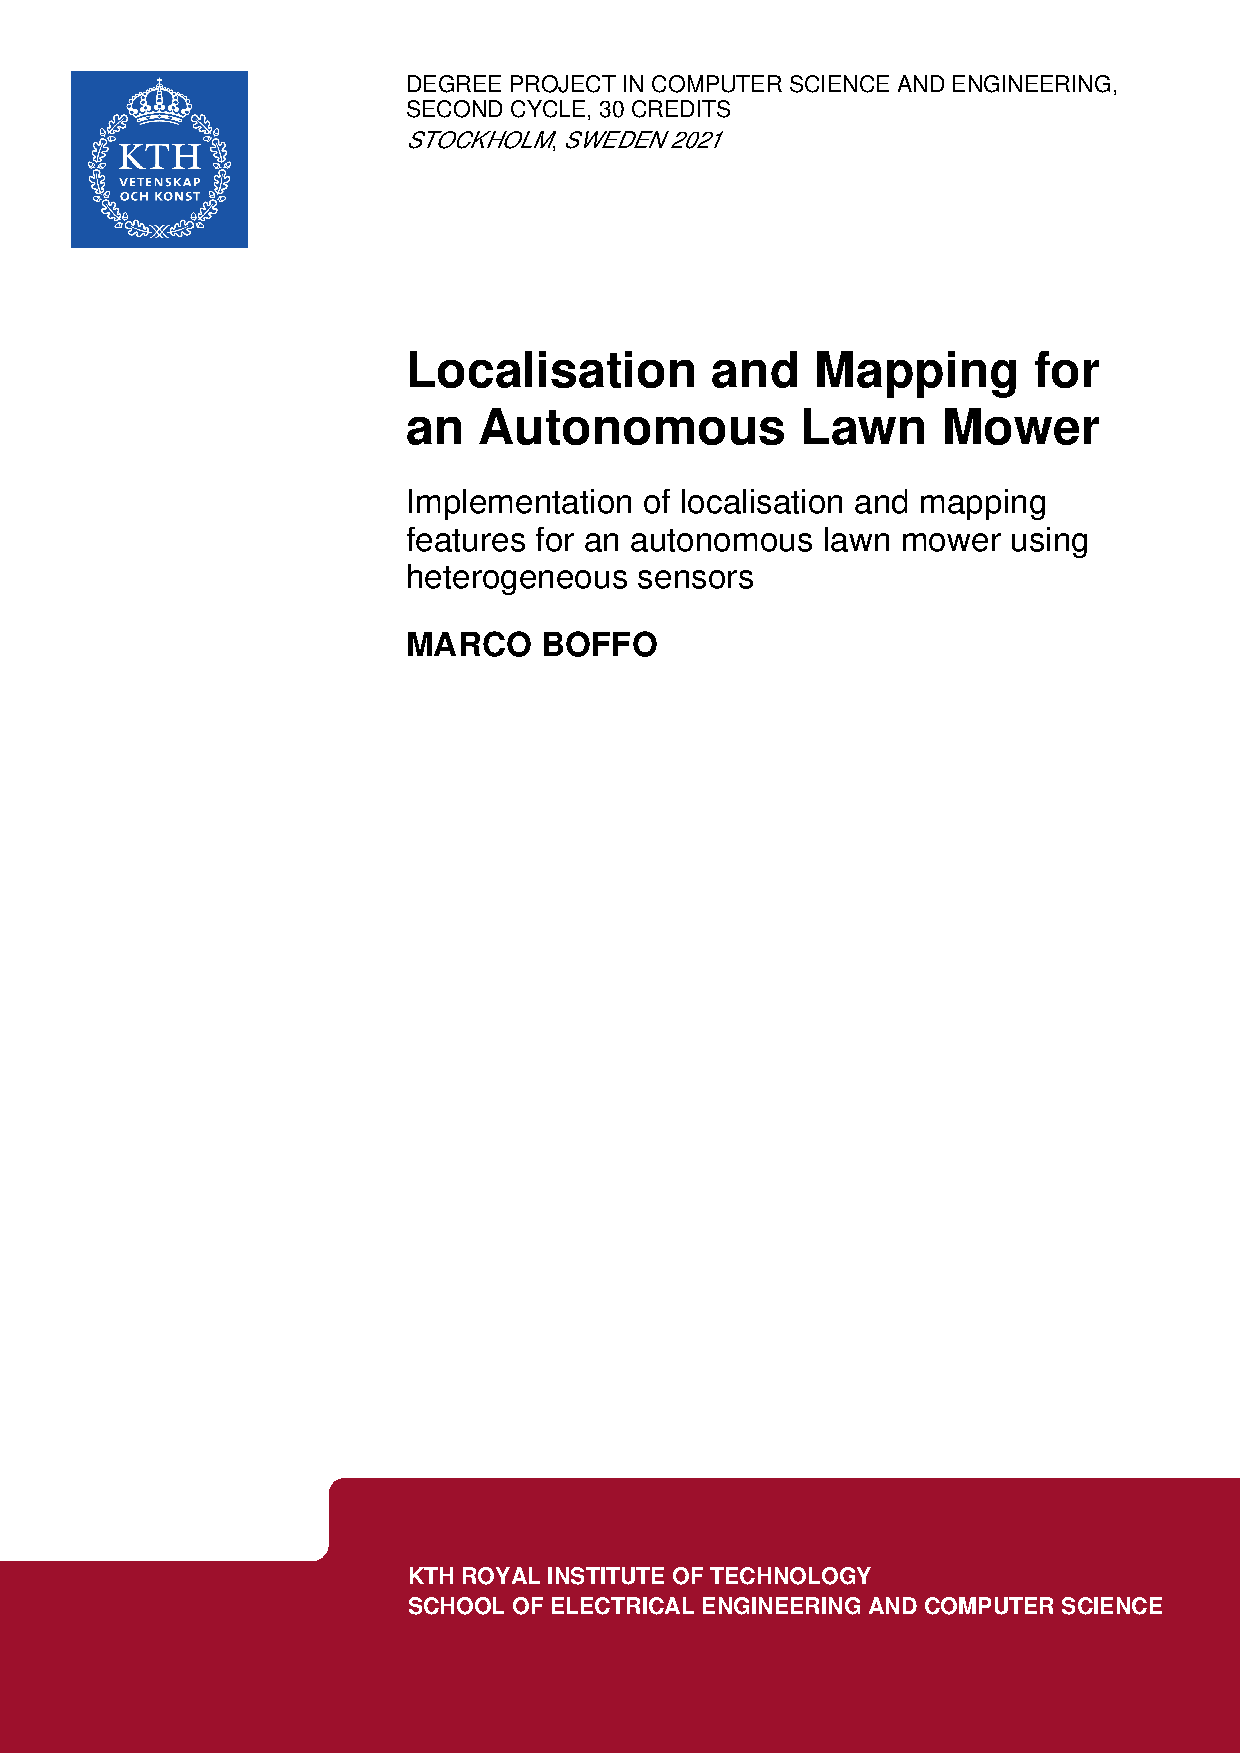
\includepdf[pages=1]{Input/kth-cover.pdf}
\newpage
\null
\thispagestyle{empty}

%% Information for inside title page
\title{Analysis of multi sensor fusion configuration for mobile robot outdoor localisation}
\subtitle{Implementation and analysis of techniques to precisely localise an autonomous mobile robot in outdoor settings by fusing measurements from multiple sensors}

% give the alternative title - i.e., if the thesis is in English, then give a Swedish title
\alttitle{Utomhus lokalisering och navigationssystem för en mobil robot}
\altsubtitle{Implementering och analys av tekniker för att exakt lokalisera och navigera i en bilkross i en utomhusgräsmatta}

\authorsLastname{Boffo}
\authorsFirstname{Marco}
\email{boffo@kth.se}
\kthid{u100001}
% If the student has an ORCiD - add it here
\orcid{0000-0003-4282-0472}
\authorsSchool{\schoolAcronym{EECS}}


\supervisorAsLastname{Carlsson}
\supervisorAsFirstname{Håkan}
\supervisorAsEmail{hakcar@kth.se}
% If the supervisor is from within KTH add their KTHID, School and Department info
\supervisorAsKTHID{u100003}
\supervisorAsSchool{\schoolAcronym{EECS}}
\supervisorAsDepartment{Intelligent Systems}
% other for a supervisor outside of KTH add their organization info
%\supervisorAsOrganization{Timbuktu University, Department of Pseudoscience}

%If there is a second supervisor add them here:
\supervisorBsLastname{Voigt}% ~~~~~- thiemo.voigt@ri.se}
\supervisorBsFirstname{Thiemo}
%\supervisorBsFirstname{~\\\hspace{2.5cm}Thiemo}
\supervisorBsEmail{thiemo.voigt@ri.se}
% other for a supervisor outside of KTH add their organization info
\supervisorBsOrganization{RISE Research Institutes of Sweden AB}


%If there is a second supervisor add them here:
\supervisorCsLastname{Eriksson}% - joakim.eriksson@ri.se}
\supervisorCsFirstname{Joakim}
%\supervisorCsFirstname{~\\\hspace{2.5cm}Joakim}
\supervisorCsEmail{joakim.eriksson@ri.se}
% other for a supervisor outside of KTH add their organization info
\supervisorCsOrganization{RISE Research Institutes of Sweden AB}

\examinersLastname{Li}
\examinersFirstname{Haibo}
\examinersEmail{haiboli@kth.se}
% If the examiner is from within KTH add their KTHID, School and Department info
\examinersKTHID{u100004}
\examinersSchool{\schoolAcronym{EECS}}
\examinersDepartment{Human Centered Technology}
% other for a examiner outside of KTH add their organization info
%\examinersOrganization{Timbuktu University, Department of Pseudoscience}


\hostcompany{RISE Research Institutes of Sweden AB} % Remove this line if the project was not done at a host company
%\hostorganization{RISE Research Institutes of Sweden AB}   % if there was a host organization

\date{\today}

\programcode{TIVNM}
%% Alternatively, you can say \programme{Civilingenjör Datateknik} to directly set the programme string

\titlepage


% document/book information page
\bookinfopage

%\listoftodos

% Frontmatter includes the abstracts and table-of-contents
%\frontmatter

\pagenumbering{Roman}
\setcounter{page}{1}


\begin{abstract}
  \markboth{\abstractname}{}

% Make first version of abstract consist of four sentences. Fill in
% more later, if needed.

% First sentence: state the problem.

% Second sentence: describe why this is a problem.

% Third sentence: state your solution.

% Fourth sentence: sketch the consequences of your solution
\com{
\todo[inline]{Keep in mind that most of your potential readers are only going to read your title and abstract. This is why it is important that the abstract give them enough information that they can decide is this document relevant to them or not. Otherwise the likely default choice is to ignore the rest of your document.\\
A abstract should stand on its own, i.e., no citations, cross references to the body of the document, acronyms must be spelled out, …\\
Write this early and revise as necessary. This will help keep you focused on what you are trying to do.}

Write an abstract\todo{Use about 1/2 A4-page (250 and 350 words).}  with the following components:
\begin{itemize}
  \item What is the topic area? (optional) Introduces the subject area for the project.
  \item Short problem statement
  \item Why was this problem worth a Master’s thesis project? (i.e., why is the problem both significant and of a suitable degree of difficulty for a Master’s thesis project? Why has no one else solved it yet?)
  \item How did you solve the problem? What was your method/insight?
  \item Results/Conclusions/Consequences/Impact: What are your key results/conclusions? What will others do based upon your results? What can be done now that you have finished - that could not be done before your thesis project was completed?\todo[inline]{The presentation of the results should be the main part of the abstract.}
\end{itemize}
}
DRAFT

\noindent
Autonomous lawn mowers have been available to consumers for more than $20$ years now.
During this lapse of time, however, their configuration and performance have seen little improvements.

With the advancement in embedded devices and sensors, such a configuration is now obsolete.
The features provided now are limited and still prone to errors.
Moreover, the installed external infrastructure on which they rely, i.e. the boundary wire, requires maintenance.

This thesis analyses the implementation of a localisation and mapping module which allows for the implementation of more features.
Multiple sensors to improve the localisation of the autonomous lawn mower are analysed, and the best configuration is presented.
Additionally, mapping features are implemented over the positioning system to update the understanding of the robot's environment.

This solution could be used to improve the coverage feature of the autonomous lawn mower.
Moreover, the availability of a more precise localisation could be the starting point for more advanced features, e.g. interaction with the lawn.



\subsection*{Keywords}
\noindent
Autonomous Mobile Robot, Sensor Fusion, Localisation, Mapping


\com{
\todo[inline]{Choosing good keywords can help others to locate your paper, thesis, dissertation, … and related work.}

Choose the most specific keyword from those used in your domain, see for example:
ACM's Computing Classification System (2012) or
(2014) IEEE Taxonomy.

Mechanics:
\begin{itemize}
  \item The first letter of a keyword should be set with a capital letter and proper names should be capitalized as usual.
  \item Spell out acronyms and abbreviations.
  \item Avoid "stop words" - as they generally carry little or no information.
  \item List your keywords separated by commas (",").
\end{itemize}
Since you should have both English and Swedish keywords - you might think of ordering them in corresponding order (i.e., so that the nth word in each list correspond) - thus it would be easier to mechanically find matching keywords.
}

\end{abstract}


%\cleardoublepage
\clearpage


\begin{otherlanguage}{swedish}

\begin{abstract}
    \markboth{\abstractname}{}

\com{
    \todo[inline]{All theses at KTH are required to have an abstract in both English and Swedish.\\
If you are writing your thesis in English, you can leave this until the final version. If you are writing your thesis in Swedish then this should be done first – and you should revise as necessary along the way.\\
If you are writing your thesis in English, then this section can be a summary targeted at a more general reader. However, if you are writing your thesis in Swedish, then the reverse is true – your abstract should be for your target audience, while an English summary can be written targeted at a more general audience.\\
This means that the English abstract and Swedish sammnfattning
or Swedish abstract and English summary need not be literal translations of each other.\\

The abstract in the language used for the thesis should be the first abstract, while the Summary/Sammanfattning in the other language can follow.\\

Exchange students many want to include one or more abstracts in the language(s) used in their home institutions to avoid the neeed to write another thesis when returing to their home institution.
}
}

DRAFT

\noindent
Autonoma gräsklippare har varit tillgängliga för konsumenter i mer än $ 20 $ år nu.
Under denna tid har dock deras konfiguration och prestanda sett små förbättringar.

Med framstegen inom inbäddade enheter och sensorer är en sådan konfiguration nu föråldrad.
Funktionerna som tillhandahålls nu är begränsade och fortfarande utsatta för fel.
Dessutom kräver den installerade externa infrastrukturen som de förlitar sig på, dvs. begränsningskabeln, underhåll.

Denna avhandling analyserar implementeringen av en lokaliserings- och kartläggningsmodul som möjliggör implementering av fler funktioner.
Flera sensorer för att förbättra lokaliseringen av den autonoma gräsklipparen analyseras och den bästa konfigurationen presenteras.
Dessutom implementeras kartläggningsfunktioner över positioneringssystemet för att uppdatera förståelsen för robotens miljö.

Denna lösning kan användas för att förbättra täckningsfunktionen för den autonoma gräsklipparen.
Dessutom kan tillgängligheten av en mer exakt lokalisering vara utgångspunkten för mer avancerade funktioner, t.ex. interaktion med gräsmattan.

\subsection*{Nyckelord}
\noindent
Autonom mobil robot, sensorfusion, lokalisering, kartläggning

  \end{abstract}
\end{otherlanguage}


%\cleardoublepage
\clearpage


\selectlanguage{italian}

\begin{abstract}
    \markboth{\abstractname}{}


\noindent
I tosaerba autonomi sono disponibili per i consumatori da oltre $ 20 $ anni.
Durante questo periodo, i progressi nei calcoli dei dispositivi integrati e nelle prestazioni dei sensori hanno portato a miglioramenti nell'affidabilità di questi robot.
Nonostante i recenti miglioramenti, l'opportunità di innovazione di tali sistemi rimane significativa.
% ciao amico questo non ha senso per me, ma rimettilo se vuoi Nonostante questo, poco sforzo è stato speso per la loro innovazione ed evoluzione relativa allo sviluppo di nuove funzionalità.

% Perché questo è un problema?
I robot autonomi hanno ancora funzionalità limitate.
Si affidano a fili elettrici installati sottoterra per delimitare i confini del prato, a cui reagiscono senza ragionamento.
Tale configurazione è ormai considerata obsoleta e sono disponibili soluzioni autonome più efficaci.

% indica la tua soluzione.
Questa tesi si concentra sull'utilizzo delle tecniche attualmente disponibili per progettare i moduli principali necessari per far avanzare le capacità di questi sistemi. % (questa frase non dice molto, è abbastanza generica... cosa stai facendo veramente? cioè progetta un filtro kalman per fare xyz)
Vengono presentate l'analisi e la relativa implementazione delle funzionalità di localizzazione e mappatura per i tosaerba autonomi.
Vengono studiati sensori eterogenei e le loro diverse configurazioni e viene proposto un filtro di Kalman adattivo esteso per fondere le loro misurazioni.
Questa tecnica migliora la stima della posa del rasaerba autonomo, che viene poi sfruttata dal modulo di mappatura.
L'approccio scelto per quest'ultimo, basato sull'inferenza bayesiana, riesce ad aggiornare la conoscenza della mappa basata su interazioni dirette con l'ambiente.

% abbozza le conseguenze della tua soluzione
I risultati finali evidenziano l'importanza di una localizzazione precisa come vero collo di bottiglia per lo sviluppo di nuove funzionalità.
La stima della posa migliorata consente la definizione di un confine virtuale. La definizione non è sufficientemente precisa per mappare correttamente la presenza di oggetti nell'ambiente
Esempi di funzionalità avanzate a partire dalla configurazione proposta sono l'implementazione di algoritmi di copertura deterministici e l'interazione con gli oggetti del prato.

\com{
I tosaerba autonomi sono disponibili per i consumatori da più di $20$ anni.
Durante questo lasso di tempo, tuttavia, la loro configurazione e le prestazioni hanno visto piccoli miglioramenti.

Con il progresso nei calcoli dei dispositivi embedded e nelle prestazioni dei sensori, la loro implementazione può essere considerata ormai obsoleta.
Le funzionalità disponibili sono limitate e ancora soggette a errori.
Inoltre, l'infrastruttura esterna installata su cui si basano, ovvero il cavo perimetrale, richiede manutenzione.

Questa tesi analizza l'implementazione di un modulo di localizzazione e mappatura.
Vengono analizzati più sensori e le loro diverse configurazioni per migliorare la stima della posa del tosaerba autonomo.
Le migliori impostazioni vengono quindi adottate con il modulo di mappatura per aggiornare una mappa con la comprensione dell'ambiente del robot.

Questa soluzione è il punto di partenza per funzionalità più avanzate aspetti avanzati.
La disponibilità di una localizzazione e definizione cartografica più precisa consente l'implementazione di algoritmi di definizione della copertura e di interazione con il prato.
}
\subsection*{Parole chiave}
\noindent
Robot mobili autonomi, fusione di sensori, localizzazione, mappatura
\end{abstract}

%\cleardoublepage
\clearpage


% set to the language of the body of the thesis
\selectlanguage{english}


\section*{Acknowledgments }
\markboth{Acknowledgments}{}
\com{
\todo[inline]{It is nice to acknowledge the people that have helped you. It is
  also necessary to acknowledge any special permissions that you have gotten –
  for example getting permission from the copyright owner to reproduce a
  figure. In this case you should acknowledge them and this permission here
  and in the figure’s caption. \\
  Note: If you do not have the copyright owner’s permission, then you cannot use any copyrighted figures/tables/… .
}
}
%I would like to thank xxxx for having yyyy.\\


DRAFT

\noindent I would like to thank Thiemo Voight and Joakim Eriksson for the opportunity to work at this challenging topic.

I would like to thank Håkan Carlsson for the supervision of the project.
His insights and suggestions have been vital for the development of this thesis.

I would like to thank Haibo Li for the examination of the thesis.

I would like to thank Mikael Alexiusson for the Husqvarna collaboration.

I want to acknowledge my family and friends that supported me through the whole process.

\acknowlegmentssignature



\fancypagestyle{plain}{}
\renewcommand{\chaptermark}[1]{ \markboth{#1}{}}


% Set depth of table of content to not care about subsections and lower
\setcounter{tocdepth}{3}

\tableofcontents
  \markboth{\contentsname}{}
%\cleardoublepage
\clearpage

%\listoffigures
%\cleardoublepage
%\clearpage

%\listoftables
%\cleardoublepage
%\clearpage

%\listofalgorithms
%\cleardoublepage
%\clearpage


%\lstlistoflistings\todo{If you have listings in your thesis.}
%\cleardoublepage
%\clearpage


%% Acronyms
%%% Local Variables:
%%% mode: latex
%%% TeX-master: t
%%% End:
% note the use of a non-breaking dash in long text for the following acronym
\newacronym{IQL}{IQL}{Independent Q‑Learning}

\newacronym{LAN}{LAN}{Local Area Network}
% note the use of a non-breaking dash in the following acronym
\newacronym{WiFi}{Wi-Fi}{Wireless Fidelity}

\newacronym{WLAN}{WLAN}{Wireless Local Area Network}
\newacronym{UN}{UN}{United Nations}

\newacronym{SDG}{SDG}{Sustainable Development Goal}

\newacronym{SLAM}{SLAM}{Simultaneous Location and Mapping}
\newacronym{ROS}{ROS}{Robotic Operating System}
\newacronym{WO}{WO}{Wheel Odometry}
\newacronym{VO}{VO}{Visual Odometry}
\newacronym{VIO}{VIO}{Visual-Inertial Odometry}
\newacronym{ICP}{ICP}{Iterative Closest Point}
\newacronym{LRF}{LRF}{Laser Range Finder}
\newacronym{DR}{DR}{Dead Reckoning}
\newacronym{UGV}{UGV}{Unmanned Ground Vehicles}
\newacronym{MEMS}{MEMS}{MicroElectroMechanical System}

\newacronym{RMSE}{RMSE}{Root Mean Square Error}
\newacronym{UWB}{UWB}{UltraWideBand}

\newacronym{EPOS}{EPOS}{Exact Positioning Operating System}
\newacronym{DOP}{DOP}{Dilution Of Precision}
\newacronym{HDOP}{HDOP}{Horizontal DOP}

\newacronym{F2F}{F2F}{Frame to Frame}

\newacronym{SIFT}{SIFT}{Scale-Invariant Feature Transform}
\newacronym{SURF}{SURF}{Speeded-Up Robust Features}
\newacronym{ORB}{ORB}{Oriented FAST and Rotated BRIEF}


\newacronym{ICC}{ICC}{Instantaneous Center of Curvature}

\newacronym{NRAO}{NRAO}{National Radio Astronomy Observatory}


\newacronym{NMEA}{NMEA}{National Marine Electronics Association}


\newacronym{API}{API}{Application Programming Interface}



\newacronym{2D}{2D}{2 Dimensional}
\newacronym{3D}{3D}{3 Dimensional}

\newacronym{IMU}{IMU}{Inertial Measurement Unit}
\newacronym{GPS}{GPS}{Global Positioning System}
\newacronym{GPSRTK}{GPS-RTK}{GPS Real Time Kinematic}
\newacronym{KF}{KF}{Kalman Filter}
\newacronym{PF}{PF}{Particle Filter}
\newacronym{EKF}{EKF}{Extented Kalman Filter}
\newacronym{IEKF}{IEKF}{Iterated Extented Kalman Filter}
\newacronym{AEKF}{AEKF}{Adaptive Extented Kalman Filter}
\newacronym{UKF}{UKF}{Unscented Kalman Filter}
\newacronym{UT}{UT}{Unscented Transform}

\newacronym{HRP}{HRP}{Husqvarna Research Platform}
\newacronym{GNSS}{GNSS}{Global Navigation Satellite System}
\newacronym{INS}{INS}{Inertial Navigation System}



\newacronym{ECEF}{ECEF}{Earth-Centered Earth-Fixed}
\newacronym{ECR}{ECR}{Earth Centered Rotation}
\newacronym{WGS}{WGS}{World Geodetic System}
\newacronym{ENU}{ENU}{East-North-Up}

\newacronym{RPi}{RPi}{Raspberry Pi}

\newacronym{RGB}{RGB}{Red Green Blue}
\newacronym{RGBD}{RGB-D}{RGB-Depth}
\newacronym{RTABMAP}{RTAB-Map}{Real-Time Appearance-Based Mapping}

\newacronym{LMSE}{LMSE}{Least Mean Squared Error}


\newacronym{DOF}{DOF}{Degree of Freedom}

\newacronym{ALM}{ALM}{Autonomous Lawn Mower}
     %load the acronyms file
\printglossary[type=\acronymtype, title={List of acronyms and abbreviations}]

%\printglossaries
%\com{
%\todo[inline]{The list of acronyms and abbreviations should be in alphabetical order based on the spelling of the acronym or abbreviation.
%}
%}
%\label{pg:lastPageofPreface}





% Mainmatter is where the actual contents of the thesis goes
\mainmatter

\renewcommand{\chaptermark}[1]{\markboth{#1}{}}

\pagenumbering{arabic}

\begin{sloppypar}
    
% Make first version of the introduction section consist of four
% paragraphs. Add paragraphs later if needed.

\chapter{Introduction}
\label{ch:introduction}

% usually 2-4 pages, you can use ``I'' or "We'' when you
% describe what you have done


% 1. Introduction to the problem and problem statement:
% why is the work needed/done, how will ``the world'' benefit from it.
% everybody with some education should be able to read this part
% and understand that the thesis is useful
% you can use sections for these parts\section{Motivation and Problem Statement}

% 2. how do you attack the problem including the method (analysis,
% experimentation etc)

% 3. other possible approaches or solutions

% 4. describe your solution and the summarize the main results,
%    if possible the research contributions

% 5: Thesis structure: outline of rest of thesis

\com{

    This\todo{The first paragraph after a heading is not indented, all of the
      subsequent paragraphs have their first line indented.} chapter describes the
    specific problem that this thesis addresses, the context of the problem, the
    goals of this thesis project, and outlines the structure of the thesis.\\

    \todo[inline]{Give a general introduction to the area. (Remember to use appropriate references in this and all other sections.)}

    at \SI{20}{cm}.
}

\noindent
Autonomous systems development has improved consistently in the later period, providing improvements to every day life.
These systems are able to autonomously execute their tasks without human interaction and to adapt to dynamic settings.
On the field of robotics, their support is relevant when tasks are repetitive and the human presence is not necessary.
In the specific case of mobile robotics, autonomous navigation is required and those systems can achieve it using knowledge of their pose and surroundings.

The pose of a mobile robot can be estimated using sensors which provide measurements of their environment.
Multiple types of sensors are available, which differ in frequency, phenomenon captured, and reliability.
Heterogeneous sensors provide measurements which need to be properly fused together to improve the individual knowledge that they provide.

The awareness and the precision related to the position in the working environment changes with respect to each application.
The first autonomous mobile robots available to the consumers were the indoor cleaning robots, where simple collision detection is enough to wander in the indoor environment.
A more recent consumer application of such robots is the \gls{ALM}, which works in the more complicated outdoor setting.

\glspl{ALM} mow the lawn using a random walk coverage approach~\cite{karol_ardic_conditional_2016}, i.e. they move in a random direction until they detect a specific underground wire or until they collide with an object.
They will then rotate towards another direction and keep on going with this behavior.
To do so, they rely in a minimal set of sensors to achieve their goals in dynamic outdoor environments.

Boundary wires are laid underground to provide the outer limits of the lawn working area, and some guide wires are used to aid the mobile robot with more complex tasks that the random behaviour will not be able to address, such as the autonomous return to the charging base and the navigation through narrow passages.
These wires transmit a proprietary electrical current signal passing through and the mobile robot is able to detect it using three different magnetometer sensors, one positioned in the center front and the other two placed on each side.
Through the analysis of the magnetic field direction and pulses, the lawn mower is able to understand if the wire defines a boundary or if it provides a guide to go towards another area of the lawn or back to the charging base.
However, these external wires require regular maintenance which could be avoided with a more sophisticated model.

Additionally, the \glspl{ALM} implement collision sensors, located near the rear wheels.
When the mobile robot bumps into any firm object from the front, it will trigger push sensors situated on the chassis.
It has been used to react in case of collision with unexpected objects, but eventually it could be used to map the environment with those objects and avoid them systematically.

In more sophisticated and recent models, additional frontal ultrasonic range sensors are installed to slow down the mobile robot before potentially colliding with objects in its trajectory.

The most advanced models also include \Glspl{GNSS} receivers to keep track of the global robot position, for theft protection and lawn monitoring purposes.
However, it is not precise enough on its own to provide real time localisation information for it to be used for navigation purposed by the \gls{ALM}, but it can be used to detect that a particular side of the lawn has not been mowed in a while.% using the random walk coverage approach.

This configuration does not require them to understand their position on the world, as they just use a reactive architecture defined by a random behaviour motion pattern without any understanding of their surroundings~\cite{wooldridge_agent_1995}.
These robots are situated, i.e. they are not taking into account events of the past and they cannot foresee their future interactions with the environment  ~\cite{muller_1999}.
As such, they are not able to plan ahead their path and they just react to perceptions of their surroundings.
They do not have a model of their world, and they do not need to update it in case of unexpected changes of their environment~\cite{wooldridge_agent_1995}.
They are flexible and adaptive as they rely on the infrastructure manually installed for them~\cite{wahde2012introduction},  which however requires additional installation and maintenance.


\com{
\section{Background}
\label{sec:background}
%Present the background for the area. Set the context for your project – so that your reader can understand both your project and this thesis. (Give detailed background information in Chapter 2 - together with related work.)
%Sometimes it is useful to insert a system diagram here so that the reader knows what are the different elements and their relationship to each other.
%This also introduces the names/terms/… that you are going to use throughout your thesis (be consistent). This figure will also help you later delimit what you are going to do and what others have done or will do.
}

\noindent 


\section{Problem}
\com{
Longer problem statement\\
If possible, end this section with a question as a problem statement.
}

\noindent
The current method of autonomously mowing the lawn is not effective, since it is based on an external infrastructure to perform a reactive behaviour based on a random walk coverage algorithm~\cite{karol_ardic_conditional_2016}.
The problems that arise from this setting are multiple, as the external components require maintenance and the current algorithm cannot guarantee a complete deterministic coverage of the area.
%Random planning cannot guarantee a complete coverage, whereas, many deterministic techniques are not solely eligible for unstructured outdoor environments, since they highly suffer from wheel slippage or numerical drift. Besides, complete coverage techniques either demands high computational power or expensive sensor hardware.
This configuration for the \glspl{ALM} was given by constraints related to the low computational power available in the past.
Moreover, the recent progresses in the performance of embedded devices and sensors have made the navigation model of \glspl{ALM} obsolete, and as those components have also lowered their cost, their implementation is now feasible even for this consumer products.
The combined availability of more advanced devices and more computational power enables for the implementation of real time applications to improve the performance of these mobile robots.


The performance of an \gls{ALM} can be improved with a more advanced perception and action system used to implement deterministic techniques of coverage planning.
The problem that needs to be solved is the development of a more precise localisation and mapping module.
The \gls{ALM}, to perceive its surroundings and act accordingly, needs additional computational power and sensors than the ones available in the current configurations.
With a more advanced set of components, it would be possible to reach a more accurate understanding of the mobile robot's pose inside a map of the lawn itself.
An analysis of the best configuration of sensors, along with their measurements fusion, is needed to understand how to provide to costumers a more reliable product which needs no maintenance of the external infrastructure.
The issue is related to finding the most appropriate technique to fuse all these sensors' measures in a setting where every downside is compensated and every useful aspect of those sensors is exploited and highlighted,


An aspect that is worth investigating is related to the removal of the need of external infrastructure used for localisation purposes.
Instead of relying to a vulnerable boundary wire and with a set of sensors built in the \gls{ALM} directly, without installing additional systems on the lawn, the implementation of such a system will allow for the offering of a more complete set of features to the users.
Additionally, the removal of such a boundary wire or external infrastructure enable the \gls{ALM} to cover larger areas of custom configuration.

Finally, the fused combination of given control commands and the whole set of sensors at disposal for this project has yet to be investigated in research, as usually fewer sensors are available.


%\subsection{Scientific and engineering issues}
%The scientific relevance of this project is derived from the fact that outdoor localisation and mapping of dynamic environments are still far from reaching a reliable solution.
%This work will aid in the handling of dynamical outdoor settings.
%Since there are just few available devices able to mow the lawn without installing additional and external devices on the lawn, this work will investigate how it can be done using a set of sensors built in the \gls{ALM} directly and removing the need for external infrastructure. This work will provide valuable insights about this heterogeneous sensor fusion.


Autonomously mowing the lawn will help saving time and avoid human intervention as much as possible.
The steps needed to improve current systems are related to a dynamic management of the boundary of the lawn, eliminating the need for a boundary wire with its related installation and maintenance.

The knowledge about position and orientation of the mobile robot, with respect to a map, enables for the application of more deliberative architectures~\cite{genesereth_logical_1987}.
With this architecture, the pose with respect to a map will allow the \gls{ALM} to make independent decisions and to plan its path to cover the lawn in a shorter amount of time, leaving a better pattern, avoiding unexpected objects, and saving energy and resources.
%The term `deliberative agent' seems to have derived from Genesereth's use of the term `deliberate agent' to mean a specific type of symbolic architecture [Genesereth and Nilsson, 1987].) We define a deliberative agent or agent architecture to be one that contains an explicitly represented, symbolic model of the world, and in which decisions (for example about what actions to perform) are made via logical (or at least pseudo-logical) reasoning, based on pattern matching and symbolic manipulation. ~\cite{genesereth_logical_1987}


\section{Research Goals}

\com{
State the purpose  of your thesis and the purpose of your degree project.

Describe who benefits and how they benefit if you achieve your goals. Include anticipated ethical, sustainability, social issues, etc. related to your project. (Return to these in your reflections in Section~\ref{sec:reflections}.)

State the goal/goals of this degree project.

This has been divided into the following three sub-goals:
\begin{enumerate}
\item Subgoal 1 \todo[inline, backgroundcolor=aqua]{för att tillfredsställa problemägaren – industrin?}
\item Subgoal 2\todo[inline, backgroundcolor=aqua]{för att tillfredsställa ingenjörssamfundet och vetenskapen – akademin) }
\item Subgoal 3\todo[inline, backgroundcolor=aqua]{eventuellt, för att uppfylla kursmålen – du som student}
\end{enumerate}

In addition to presenting the goal(s), you might also state what the deliverables and results of the project are.
}

\noindent
This master thesis investigates how to improve the performance of an \gls{ALM} providing localisation and mapping features using a set of heterogeneous sensor directly mounted on it.
It will focus on the implementation and analysis of a module based on the fusion of the measurements provided by different configurations of those sensors to remove the need of relying on external infrastructure.
%An overview of the best settings for a precise localisation is provided
%Different configurations of sensors and techniques to fuse their measurements are investigated to provide an overview of the best setting to improve the localisation performance.
Finally, their configurations are investigated through multiple experiments, and drawbacks and improvements of each sensor are analysed.

The goal of this thesis is to provide an overview on how to develop a precise localisation module for an \gls{ALM}.
An analysis about different configurations of sensors and about how to fuse their measures using sensor fusion filters is presented.
As end result, the \gls{ALM} is able to operate in a specified environment without the need to intervene with the installation of additional infrastructure, but just with the addition of heterogeneous sensors installed directly on the mobile robot.

The focus of this degree project is the precise localisation inside a predefined given map to ensure that the \gls{ALM} stays inside the virtual boundaries defined.
Moreover, a map of the lawn is developed to allow for updates using collision events against unexpected object to provide a more dynamic view of the lawn.
%It will benefit both the industry of \gls{ALM} with the knowledge derived from this thesis, and the consumers will obtain a product which requires less maintenance.

The research questions to be evaluated are the following:
\begin{itemize}
    \item Providing an initial map and location of the \gls{ALM} in it, will the \gls{ALM} be able to stay within the given boundaries with a specified margin for error?
    \item Will the \gls{ALM} be able to correctly update the map by adding or removing eventual obstacles found by navigating in the map through collision detection?
\end{itemize}

In order to evaluate if the above goals have been reached, for an \gls{ALM} made to cover an area of \SI{5000}{\meter\squared}, the following measurable objectives will be adopted:
\begin{itemize}
    \item Identify if the mobile robot is able to stay within the boundaries defined, ensuring that the error in boundary violation will be inside the dimension of the \gls{ALM} itself: around \SI{50}{\cm}.
    These measures are defined to show that the lawn mower will not exceed its given boundaries, risking to damage itself, the lawn, or others.
    \item Identify if the \gls{ALM} is able to return to the parking dock to recharge itself with an offset of a maximum of \SI{1}{\m} after a run of at least \SI{500}{\m}. In this way, it will be relevant to show how the mobile robot is not drifting.
    Moreover, with this results it will be possible to correct eventual offsets once at the starting position.
    \item Identify if the \gls{ALM} is able to localise a collision event within an error of at most $1\%$ of the total distance already travelled, e.g. identify a tree with a maximum offset of \SI{20}{\cm} error after a \SI{20}{\m} run.
    This will be addressed to ensure that the mower is able to update precisely the map with the presence of unexpected objects.
\end{itemize}


\com{
(Return to these in your reflections in Section~\ref{sec:reflections}.)
}

\section{Research Methodology}
\com{
Introduce your choice of methodology/methodologies and method/methods – and the reason why you chose them. Contrast them with and explain why you did not choose other methodologies or methods. (The details of the actual methodology and method you have chosen will be given in Chapter~\ref{ch:methods}. Note that in Chapter~\ref{ch:methods}, the focus could be research strategies, data collection, data analysis, and quality assurance.)\\
In this section you should present your philosophical assumption(s), research method(s), and research approach(es).
}

\noindent
The research methodology~\cite{RESEARCHMETHOD} will follow a quantitative approach: acquiring measurements and using them to validate or not the formulated research questions through quantitative analysis.
The assumptions will follow an objective and realistic paradigm where the final results will be evinced quantifying measures of the observations and gaining a better knowledge of the environment.
The research method adopted will be of experimental nature to understand the cause and effect of the obtained measurements, improving where possible, and of descriptive nature to highlight the characteristics of the obtained system.
A deductive approach will be used to test the theories and draw conclusions about the hypotheses described in the research questions.
The research strategy adopted will be based on data collection through multiple case studies of experimental nature and the collected data will be analysed with computational mathematics.
Statistical analysis will be used to test the quality of the obtained results.
In particular, in this degree project, I will apply and discuss the validity, reliability, replicability, and ethics of those results.

The following tasks are required to achieve the above mentioned objectives.
Literature study is the first step.
The next step is related to the improvement of the available localisation module performance, starting from the refinement of the sensor's drivers.
The most relevant sensor fusion technique identified is implemented to merge heterogeneous sensors' measurements.%, improving the accuracy of the localisation performance.
Afterwards, different configurations of sensors are tested and a phase of tuning their attributes to reach more reliable and valid results is done.
The theoretical validation of the sensor fusion system is performed with the usage of simulations of the sensor's measurements according to the required assumptions.
Some outdoor experiments are performed and checked against the ground truth with some metrics to evaluate the improvements on the localisation performance.
Finally, relying on the localisation results, the definition of initial virtual boundary is going to be provided with a first run of the \gls{ALM}.
The knowledge of the elements inside the obtained map is then improved using collisions events, always relying on the localisation improvements.

\begin{figure}[!ht]
	\begin{center}
		\begin{tikzpicture}[font=\small,thick]

			\node[draw,text centered,fill=green!30,rounded corners,
			align=center,
			minimum width=2.5cm,
			minimum height=1cm,
			] (block0) { System \\ Configuration};

			\node[draw,text centered,fill=cyan!30,rounded corners,
			right=of block0, align=center,
			minimum width=2.5cm,
			minimum height=1cm,
			] (block1) { Localisation \\ Improvements };

			\node[draw,text centered,fill=cyan!30,rounded corners,
			right=of block1, align=center,
			minimum width=2.5cm,
			minimum height=1cm,
			] (block2) { Mapping \\ Features };

			\node[draw,text centered,fill=red!30,rounded corners,
			right=of block2, align=center,
			minimum width=2.5cm,
			minimum height=1cm,
			] (block3) { Path \\ Planning};

			% Arrows
			\draw[-latex] (block0) edge (block1);
			\draw[-latex] (block1) edge (block2);
			\draw[-latex] (block2) edge (block3);
		\end{tikzpicture}
	\caption[Caption]{Main tasks of the project:~\\
	Improvement[green], new development[blue], and future development[red].\centering}
	\end{center}
	\label{fig:Maintasks}
\end{figure}


\com{
\subsection{Scope}
Describe the boundary/limits of your thesis project and what you are explicitly not going to do. This will help you bound your efforts – as you have clearly defined what is out of the scope of this thesis project. Explain the delimitations. These are all the things that could affect the study if they were examined and included in the degree project.
\noindent
}

Since such \glspl{ALM} are consumer products, some constraints will be taken into account, such as the configuration complexity and the sensors' cost analysis.
Some aspects regarding this degree project are described here:
\begin{itemize}
    \item The operation area is projected into a \Gls{2D} environment.
    \item The usage of an embedded device, such as a \gls{RPi}, limits the computational power of the module. Thus, the performance might not be as good as if a more powerful device would be used. %In this project, this aspect of optimization of the limited resources available on an embedded system will not be investigate.
    \item A complete \gls{SLAM} algorithm is too computationally expensive to perform well in real-time with considering a dynamic outdoor environment.
    Instead, an easier approach is to split the two different phases.
    The localisation aspect will be achieved with a sensor fusion approach and the mapping happens after localisation, using collision events to update the knowledge of the predefined map.%receiving directly a predefined map layout configuration of the environment with a given starting point of the \gls{ALM} should ease the process of  within it.
    \item Relying on a camera in outdoor settings means that the weather conditions and time of mowing can affect the results.
    As such, the testing will be performed in similar configurations, and, if possible, with an attitude towards limiting such a characteristic.
    \item A Range Finder Sensor was not considered as most of the outdoor environment will be sparse or empty.
    Thus, the sensor would not be able to provide valuable improvement to justify the expensive choice.
    Moreover, such a sensor requires a relevant amount of computational power to be run.
\end{itemize}
They provide the rationale for the project to investigate some aspects more than others.
Some of them are directly limiting and they are not be investigated for such a project.
Some others instead are part of the future works, discussed at the end of this thesis.


\section{Structure of the thesis}
\noindent In the following chapters the topics of this thesis are discussed as follows.

%Chapter~\ref{ch:introduction}, Introduction, presents briefly the background, the problem, and how it will be solved.
%The chapter also presents an overview about competitors' approaches regarding improvements of \gls{ALM} performance.

Chapter~\ref{ch:background}, Background, presents relevant information about mobile robots, localisation, and mapping.
Some theoretical related works are presented to describe the state-of-the-art.
It provides a summary about the lesson learned during the literature review.

Chapter~\ref{ch:methods}, Methods, defines the localisation and mapping approaches chosen from the literature study.
Moreover, the methodologies and experiments configurations to achieve the research goals are explained.

Chapter~\ref{ch:whatYouDid}, Implementation, presents the system implementation adopted to test the system.
It also motivates and elaborates on the implementation of the hardware and software required to run the system.

Chapter~\ref{ch:results}, Experiments and Results, defines the experiments developed to address the research questions.
Moreover, the quantitative results obtained from them are shown to highlight the desired aspects.

Chapter~\ref{ch:discussion}, Discussions, explains and interprets the final results.
The findings and their limitations are elaborated on.

Chapter~\ref{ch:conclusion}, Conclusions, wraps up the thesis and  how to improve further are provided.
Finally, some reflections related to this thesis are presented.


\cleardoublepage
%\clearpage


    \chapter{Background}
\label{ch:background}

% material necessary to understand the rest of the thesis

% last section in this chapter is usually related work

\com{
\todo[inline]{When you do your literature study, you should have a nearly complete Chapters 1 and 2.\\
You may also find it convenient to introduce the future work section into your report early – so that you can put things that you think about but decide not to do now into this section.\\
Note that later you can move things between this future work section and what you have done as you may change your mind about what to do now versus what to put off to future work.
}

What does a reader (another x student -- where x is your study line) need to know to understand your report?
What have others already done? (This is the “related work”.) Explain what and
how prior work / prior research will be applied on or used in the degree
project /work (described in this thesis). Explain why and what is not used in
the degree project and give valid reasons for rejecting the work/research.
}


\noindent This chapter presents relevant research background needed to understand the current state of the art of localisation and mapping.
Firstly, the coordinate frames of the wheeled mobile robot are presented to define how the robotic lawn mower will be localised, controlled, and constrained.
Afterwards, the focus will be on localisation, starting from an analysis of sensors available on \glspl{ALM} and other useful for positioning in outdoor settings.
The focus is on sensors which require no additional infrastructure installation.
Additionally, sensor fusion techniques to exploit their measurements will be presented to later explain which technique is the most relevant for this project.
Furthermore, a brief analysis of mapping aspects is presented.
Different algorithms are available, but only the most relevant approach is discussed.
Finally, theoretical related works are briefly described to highlight their contributions regarding this thesis, and a summary of the lessons learned from the literature study is presented.


\section{Wheeled Mobile Robots}

\noindent Mobile robots are able to move themselves in the environment they are in.
The one used in this thesis equips two standard back wheels with differential drive and two castor wheels on the front, which allow free rotation around the wheel axle for multiple direction steering.
An analysis of the coordinate and robot frame is presented, followed by the definition of its kinematic model and related constraint.

\subsection{Coordinate Frame}

\noindent
The \gls{2D} pose of the robot, ${pose}$, in the global frame $G$ is defined by the following vector:
\begin{equation}
    pose = \begin{bmatrix}x_{pose}&y_{pose}&\theta_{pose}\end{bmatrix}^T
    \label{eq:dof}
\end{equation} where the coordinates $x_r$ and $y_r$ define the position of $O_R$ in $O_G$, and $\theta_r$ defines the relative rotation angle between the $X_R$ direction axis of the robot and the related global axis $X_G$, as shown in figure \ref{fig:TikzKine}.
\begin{figure}[!ht]
    \centering
\begin{tikzpicture}
  \draw [<->, very thick]  (0,8) node (yaxis) [above] {$Y_G$} |- (10,0) node (xaxis) [right] {$X_G$};
  \draw (-0.4,-0.4)  node (origin) [] {\large$O_G$};
  \draw (4,-0.3)  node (x_r) [] {\large$x_R$};
  \draw (-0.3,3)  node (y_r) [] {\large$y_R$};
  
  \draw (8,-0.4)  node (x_i) [] {\large$x_G^P$};
  \draw (-0.4,6.5)  node (y_i) [] {\large$y_G^P$};
  \draw (8.3,6.8)  node (p) [] {$P$};
  \fill[black]  (8,6.5)   circle (2pt);
  \draw[ loosely dashdotted] (8,0) -- (8,6.5);
  \draw[ loosely dashdotted] (0,6.5) -- (8,6.5);
  
  \draw[black] (0, 0) circle (0.2) node (z) [below] {~~$~~~~~Z_G$};
  \fill[black]  (0,0)   circle (2pt);
  \draw[ densely dashed] (4,0) -- (4,3);
  \draw[ densely dashed] (0,3) -- (4,3);
  \begin{scope}[xshift=113.5, yshift=85]
        \fill[black]  (0,0)   circle (2pt);
          \draw [<->, loosely dotted]  (0,4.5) node (yaxisG) [above] {$Y_G^{'}$} |- (5.5,0) node (xaxisG) [right] {$X_G^{'}$};
          \draw (-0.4,-0.4)  node (origin_r) [] {\large$O_R$};
          \draw[->, densely dashed]  (2.5,0) to[out=60,in=-30, distance=0.5cm] (2.17,1.25) node (theta) [below, right] {\large$~~\theta_r$} ;
      \begin{scope}[rotate=30]
          \draw [<->, loosely dotted, thick]  (0,5.5) node (yaxis_r) [above] {$Y_R$}
                |- (6.5,0) node (xaxis_r) [right] {$X_R$};
          \draw[->, thick]  (0.5,-0.5) to[out=45,in=-45] (0.5,0.5)  node (omega) [above] {\large$~\omega$} to[out=135,in=45] (-0.5,0.5);
          \draw [->, thick] (0,0) -- (2,0) node (vel) [above, left] {\large$v$~~};
          \draw [->, thick] (0,2) -- (1.25,2) node (v_L) [below] {\large$\dot \delta _L$~~};
          \draw [->, thick] (0,-2) -- (1.25,-2) node (v_R) [below] {\large$\dot \delta _R$~~};
          \draw[<->, thick]  (-2,-2) -- (-2,2) node (base) [pos=0.5, below, left] {$~B_W$} ;
          \draw[<->, thick]  (-0.75,2.75) -- (0.75,2.75) node (diameter) [above, left] {$W_D$~~} ;
          \draw[<->, thick]  (-1.75,0) -- (-1.75,4.5) node (curvature) [pos=0.6, below, left] {$R$} ;
          \draw[-, loosely dashed]  (0,-2) -- (0,4.5) ;
            \fill[black]  (0,4.5)   circle (2pt);
            \draw (0,4.5)  node (ICC) [above, right] {$ICC$};
        \draw[black]  (-0.75,-2.33) rectangle (0.75,-1.67);
        \draw[black]  (-0.75,2.33) rectangle (0.75,1.67);
        \draw[black] (-1.5,-2) rectangle (3.5,2);
        \draw[black] (2.75, 1.25) circle (0.3);
        \draw[black] (2.75, -1.25) circle (0.3);
        \draw[black] (0, 0) circle (0.2) node (z) [below] {~~$~~~~~~~~Z_R$};
        
        
          \draw (5.25,-0.4)  node (x_i) [] {\large$x_R^P$};
          \draw (-0.4,1.05)  node (y_i) [] {\large$y_R^P$};
          \draw[ loosely dashdotted] (5.25,0) -- (5.25,1.05);
          \draw[ loosely dashdotted] (0,1.05) -- (5.25,1.05);
      \end{scope}
  \end{scope}
\end{tikzpicture}
  \caption{Kinematic model of a differential drive mobile robot.}
  \label{fig:TikzKine}
\end{figure}

The translational and rotational relations from a robot frame point $P_R=[x_R^P,y_R^P,1]^T$ to its global corresponding $P_G=[x_R^G,y_R^G,1]^T$ are defined by the transformation matrix $T^G_R$.
\begin{align}
P_{G} = T^G_R \cdot P_{R} && \text{with } && T^G_R =
\begin{bmatrix}
\cos(\theta_r) & -\sin(\theta_r) & x_R \\
\sin(\theta_r) & \cos(\theta_r) & y_R \\
0 & 0 & 1 \\
\end{bmatrix}
\label{eq:transfPoint}
\end{align}
Every roto-translation of points in the \gls{2D} plane is uniquely defined by the equations~\ref{eq:transfPoint}.  
Other transformation matrices are not relevant for the case study.


\subsection{Kinematic Analysis}
\label{ssec:kin_a}
\noindent
For the scope of this thesis, the kinematics are considered. Other aspects, such as torque, friction, physical implications, and in general the dynamics of the systems, are not relevant to be analysed for the scope of this thesis.

The direct kinematic equations are defined as follows.
The \gls{ALM} consists of two drive back wheels mounted along the same axis.
Each wheel is actuated independently either in forward or backward rotation.
By individually setting the velocity of each wheel, the robot rotates around a different \gls{ICC}~\cite{ICC}, $ICC$ in figure \ref{fig:TikzKine}.
This point is defined in the $Y_R$ axis by its distance, $R$, from the robot's origin:
\begin{equation}
    R = \cfrac{\dot \delta_R + \dot \delta_L}{\dot \delta_R - \dot \delta_L} \cdot \cfrac{B_W}{2}
    \label{eq:R}
\end{equation}
where $\dot \delta_R$, $\dot \delta_L$ are the perceived velocities of the right and left wheel respectively, and $B_W$ defines the base width of the \gls{ALM} as distance between the wheels.
Using this approach it is possible to vary the trajectory that the robot follows by varying the wheels' velocities.
In case the wheels' velocities are equal, $R$ will result to be infinite and the robot will not rotate, following a straight trajectory.
%Some constraints about the possible trajectories are explained in section \ref{sec:constraints}.
The rate of rotation about $ICC$ is the same as the angular velocity around the robot frame's origin $O_R$, defined by the time derivation of its orientation $\theta_r$. 
This angular velocity, $\omega$, is used to control the trajectory of the robot and its derivative is defined as:
\begin{equation}
    \omega = \cfrac{\partial{\theta_r}}{\partial{t}} = \cfrac{\dot \delta_R - \dot \delta_L}{B_W}
    \label{eq:omega}
\end{equation}
where $\partial{t}$ is the partial timestamp used to derive the velocity from the partial angle displacement $\partial{\theta_r}$.

The \gls{ALM} is controlled through the desired linear velocity $v$ along the $X_R$ axis of the robot, and the desired angular velocity $\omega$ around the $Z_R$ axis.
The angular velocity is defined above in equation \eqref{eq:omega} and the linear velocity can be defined as a transformation of either the angular velocity or the wheels' velocities, as in:
\begin{equation}
    v = \omega \cdot R = \cfrac{\dot \delta_R + \dot \delta_L}{2}
    \label{eq:vel}
\end{equation}

The inverse kinematics are defined as follows.
The \gls{ALM} model is controlled by differential drive kinematics as it is propelled by two separate motors mounted on the back wheels, and its movements are defined by the wheel actuators. The desired control velocities need to be transformed into the wheels' velocities using:
\begin{align}
    \dot \delta _L  & = v - \omega \cdot \frac{B_W}{2} & , &&
    \dot \delta _R  & = v + \omega \cdot \frac{B_W}{2} \quad .
    \label{eq:wheel_vel}
\end{align}


\subsection{Constraints}
\label{sec:constraints}
\noindent
This differential drive system is not able to move immediately in every direction along the \gls{2D} environment.
The degrees of freedom, defined in \eqref{eq:dof}, are fewer than degrees of mobility, given by the control velocities, $v$ and $\omega$.
The system is thus called non-holonomic and at least a non-holonomic constraint has to be defined for it.
A non-holonomic rolling constraint could be set for the standard wheels used by the differential mobile robot, as the wheels spin purely along their orientation.
For example, to allow the robot to perform a rolling motion along the $Y_R$ axis, the robot will have to vary the velocity of each wheel to rotate around its origin, aligning itself along that desired direction, before moving forward.

Non-holonomic constraints do not allow for the integration of the differential equations to retrieve the final pose, since the displacements of each wheel are not sufficient to determine it.
This implies that the position and orientation need to be estimated using the integration of wheels' velocities, rather than their position displacements.
An integrable approach can be used to estimate its pose with a sufficient sampling rate, but the usage of incremental displacements provided by integration of wheels' velocity measurements will inevitably accumulate errors over time, causing a drift on the pose estimates.

\com{
\section{Localisation}
\noindent As this is the main topic of this project, an extensive analysis of this field will be performed.
Understanding the current state-of-the-art of localisation and its possible improvement is required.

Firstly, the available sensors that could be installed directly on the mobile robot, that do not require additional installation of infrastructures, and that can be used to improve localisation are described below.

Afterwards, different techniques available to fuse their heterogeneous measurements are described in their performances.
}

\section{Sensors}
\noindent For a robot to localise itself, it needs to perceive its surroundings using measurements of its sensors, which perceive and interpret different phenomena based on their characteristics.
They can be classifies into two main different types~\cite{perception}.
\textit{Proprioceptive sensors} measure values internal to the robot's system, while it interacts with the environment. They provide a value of how the movements of the mobile robot are perceived with respect to the outside, e.g., wheel encoders, accelerometers, or gyroscopes.
\textit{Exteroceptive sensors} provide measurements related directly to their perception of the robot's environment. The information they measure are related to phenomena happening at the environments around the mobile robot, e.g., magnetometers, \glspl{GNSS}, or cameras.
As they measure different aspects, their capabilities differ based on the phenomenon they measure and on the .
They provide different sampling rates and measured states, which need to be combined to exploit their characteristics and limit their inaccuracies.

An overview is presented below to introduce the available sensors installed on the \gls{ALM} and adopted to improve localisation.

\subsection{Wheel Encoder}

\noindent This proprioceptive sensor detects the number of revolutions of the wheels, and they can be used to estimate their velocity~\cite{encoder}. An example of an optical wheel encoder is given in Figure \ref{fig:encoder}.
\begin{figure}[!ht]
  \begin{center}
    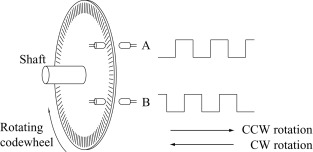
\includegraphics[width=0.65\textwidth]{Images/2-Background/Enc.jpg}
  \end{center}
  \caption{Optical wheel encoder and resulting encoded signal~\cite{wheelEncoder}.}
  \label{fig:encoder}
\end{figure}

This sensor relies on a rotary encoding disk attached to the wheel axis on the end of the motor that estimates the relative angle change of the wheel.
Rotary encoders can be of different kinds based on which phenomenon they observe: mechanical, optical, or magnetic.
Incremental encoders estimate the relative rotation of the wheels by detecting the number of pulses, defined by the step signals A and B in Figure \ref{fig:encoder}, within certain time period using the internal clock of the embedded computer.

Wheel encoders are often chosen for the estimation of the pose, as their measurements can be used through integration with the previous estimate of the robot's pose to provide the next pose estimate.
This process is called \gls{DR} and the pose estimate provided is called \gls{WO}.
Related to the field of sensor fusion, since they provide measurements with an high sampling rate and they are inexpensive, their employment is common to compute a short-term accurate \gls{DR}.
However, it is subjects to errors and their accumulation, given that only velocity measurements are used.
Some non-systematic errors related to these sensors are the miscalculations caused by slippage, uneven terrain, and other environmental issues which include wheels' temperature and the pressure of their tires.
In order to improve its \gls{DR} estimates, other sensors' measurements need to be combined with its velocity estimates to get rid of the integration drift error accumulation on its position calculations.


\subsection{Inertial Measurement Unit}

\noindent An \gls{IMU} is an inertial sensor which is used to detect multiple phenomena and whose measurements are relative to the inertial frame of the platform they are attached to.
They perceive both proprioceptive elements through accelerometers and gyroscopes, and exteroceptive characteristics through magnetometers.
Recent \glspl{IMU} are developed on \glspl{MEMS} which are inexpensive and provide measurements with high sampling rates.
These sensors are placed in each orthogonal axis to provide measurements for each degree of freedom in free space, as shown in Figure \ref{fig:imu}.
\begin{figure}[!ht]
  \begin{center}
    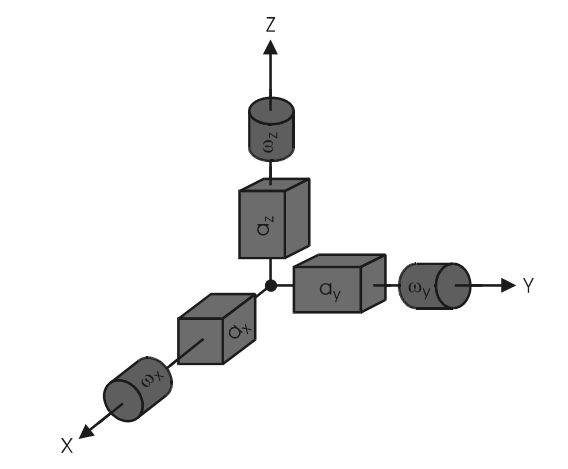
\includegraphics[width=0.5\textwidth]{Images/2-Background/IMU-2021-04-23 14-13-19.png}
  \end{center}
  \caption{Structure of accelerometers and gyroscopes of an \Gls{IMU}~\cite{inertial}.}
  \label{fig:imu}
\end{figure}

Accelerometers measure linear acceleration, gyroscopes output the perceived angular velocity, and magnetometers provide measurements about the surrounding magnetic field.
Knowing these quantities, the position and orientation can be estimated by integrating those signals over time with a \gls{DR} approach~\cite{indr}.
Their measurement are prone both to deterministic errors, such as repeatable terms and temperature induced variations, and to stochastic errors, such as switch-on to switch-on variations and in-run variations~\cite{magnusson_improving_2012}.
Deterministic errors can be compensated for through prediction and calibration, while stochastic ones are more difficult to model because of their noise and randomness.

Accelerometers and Gyroscopes, as they measure proprioceptive characteristics, are sensors that provide measurements which are not conditioned by external conditions or disturbances.
Magnetometers, instead, might be conditioned by external disturbances as the magnetic field can be affected by multiple external factors, as any electronic device has a magnetic influence.

They provide accurate results over a short time span, but the integration of noisy measurements implies an accumulation of these errors over time. This phenomenon then leads to a diverging drift effect, if not corrected by other sensor measurements.


\subsection{Global Navigation Satellite System}

\noindent \glspl{GNSS} are exteroceptive systems based on signals received from satellites orbiting earth.
A \gls{GNSS} receiver uses trilateration to estimate its position on the globe using the time of flight of the signals sent by specific satellites.  %, used to calibrate the \gls{3D} pose and time difference. 
The messages sent by them include their trajectories and their internal reference timestamp. 
As soon as the position and time difference are known, those are used to estimate the pose of the robot using pseudo-ranges, as shown in Figure \ref{fig:gps}.
\begin{figure}[!ht]
  \begin{center}
    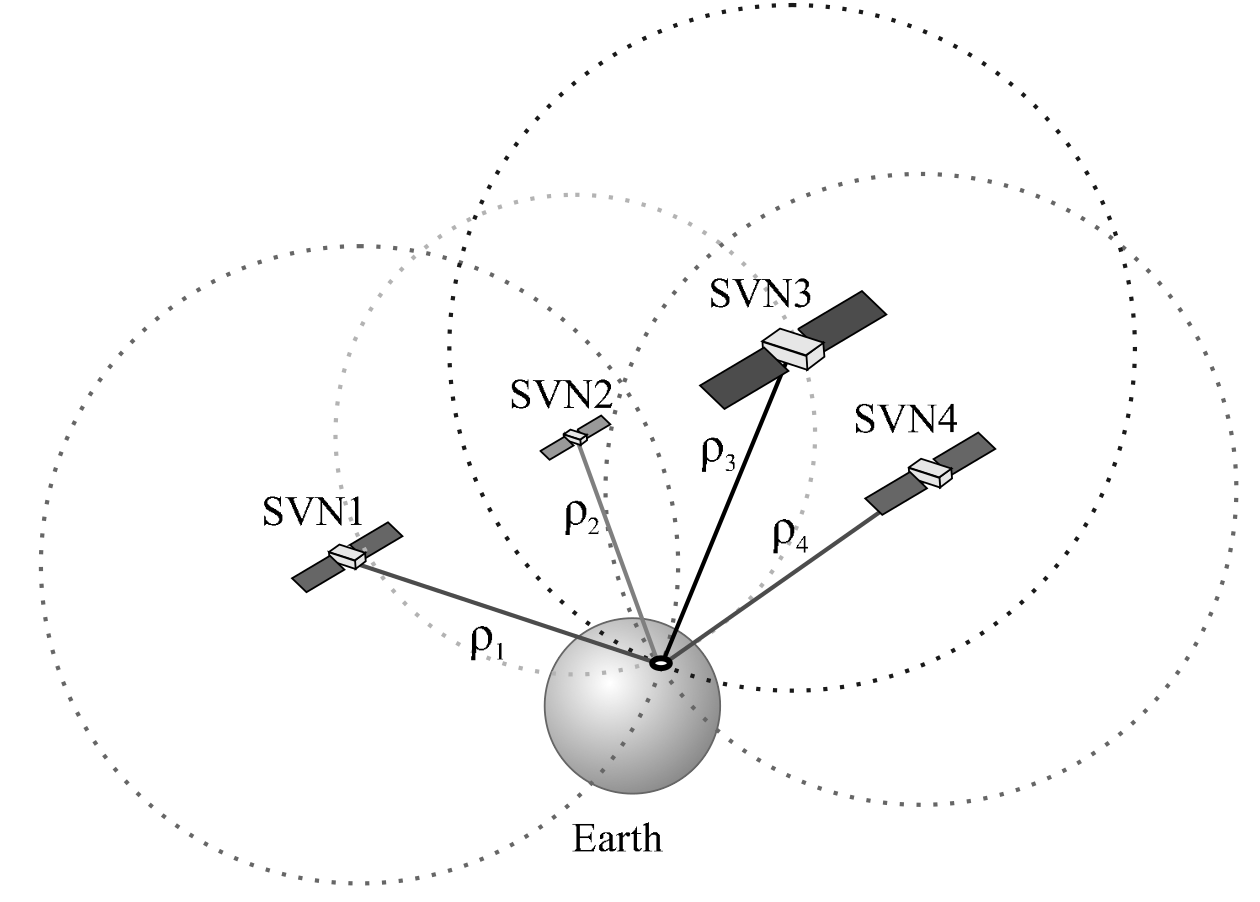
\includegraphics[width=0.5\textwidth]{Images/2-Background/KaiBorre-p73.png}
  \end{center}
  \caption{\Gls{GNSS} trilateration from known position of four satellites~\cite{Borre2007}.}
  \label{fig:gps}
\end{figure}

The spatial configuration of the satellites determines the localisation accuracy. 
Close position of several satellites implies that their range will be close, and the messages they provide will not be as useful for trilateration.
A more spread configuration of satellites' range reduces the \gls{DOP}, which compares the position error to the satellite range error.
Other source for error is related to the positioning in dense and noisy environments, due to multi-path effects of the signals.
The performance of these sensors is thus highly dependent on their environment.

For the \gls{GNSS} receiver to estimate its position, it need to acquire measurements from at least four satellites~\cite{Borre2007}.
The four satellites signals are used both to trilaterate the \gls{3D} position and to synchronise of the clocks, essential to compensate eventual time differences between the receiver and the satellites.
In case the perceived satellites are fewer than four, the receiver will have a system outage, not being able to estimate its position and velocity.
As now there exists multiple \gls{GNSS} constellations developed by distinct space agencies, the latest \gls{GNSS} sensors are able to receive signals from multiple satellite systems to improve their satellite coverage and their precision.
With a higher number of perceived satellite signals, the receiver is able to use redundant information to increase its robustness to external disturbances and improve its position measurement accuracy.

The sampling rate of \gls{GNSS} receivers is usually \SI{1}{Hz}, thus, used alone it is too slow for real-time applications of positioning for vehicles. 
However, it offers global measurements, which are not subject to drift errors and therefore they can be used to correct \gls{DR} estimates.


\subsection{Camera}

\noindent A camera sensor is an exteroceptive sensors, usually composed of lenses and light sensors, which gathers the \gls{RGB} information from the environment.
Recent camera models, e.g., structured-light cameras, are also able to estimate depth measurements. %estimate stereopsis data, used
They project an infrared mesh pattern in the environment and then use stereo cameras to perceive this pattern, trilaterating the depth distance based on the density of the projected points.
Multiple factors can lower this sensor's performances, such as excessive lightning conditions and reflecting materials which modify the infrared pattern.

These sensors provide \gls{VO} estimating the incremental movement of the camera by detecting changes in adjacent images with a \gls{F2F} method~\cite{camera}~\cite{cameraa}.
The \gls{VO} algorithm identifies the position of some specific features and then matches those landmarks in consecutive images.
Knowing their relative pose changes it is possible to estimate the corresponding camera movement.
The performance relies on the identification of landmarks, the more visible and variant landmarks are identified, the more the pose estimation will be accurate as the landmarks' difference will be more prominent.
%Those features can be computed using different descriptors, e.g. \gls{SIFT}, \gls{SURF}, or \gls{ORB}.
The matching phase is guided by an initial estimate of the camera movement which projects previously found features to search just along that projection.
The landmarks are matched after passing a consistency test and those displacements are triangulated to estimate the camera pose through a bundle adjustment step~\cite{robustFusion}, as shown in Figure \ref{fig:camera}.

\begin{figure}[!ht]
  \begin{center}
    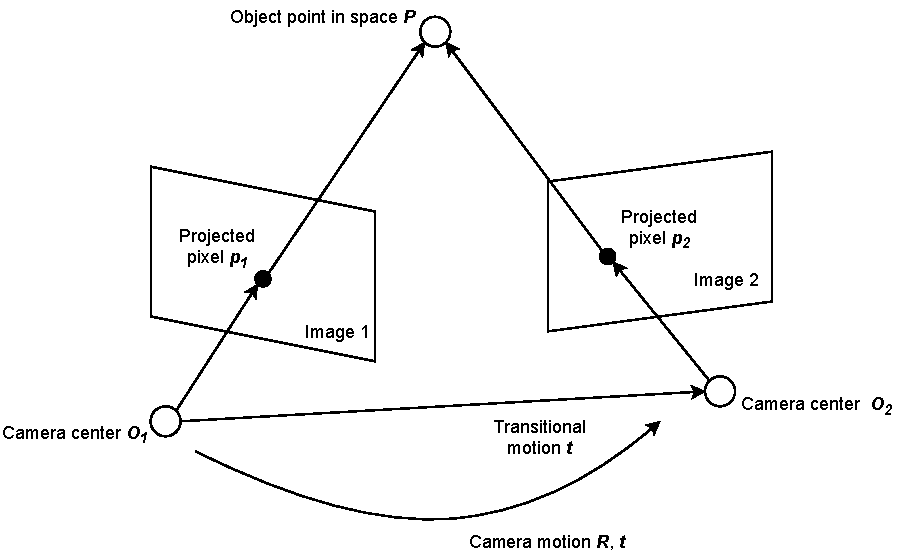
\includegraphics[width=0.65\textwidth]{Images/2-Background/VO.pdf}
  \end{center}
  \caption{Motion estimation via \gls{F2F} methodology~\cite{camera}~\cite{cameraa}.}
  \label{fig:camera}
\end{figure}

Instead of using a more complex \gls{SLAM} algorithm, where all the position of the landmarks are also used to estimate a map of the environment, with the \gls{VO} approach the landmarks are only used for displacement analysis, without storing the landmark positions over time.
Using this technique, only the previous state will be saved to estimate the position offset, resulting in faster computations and thus higher sampling frame rates.
This is a key aspect, since the aim is to use this approach inside an embedded system for a real-time application. 
However, the measurements provided from the \gls{VO} are estimates in velocity between frames and they need to be integrated to compute a \gls{DR} localisation, which is subject to drift.

%Different techniques are available to compute the features and derive the estimations from the frames, with different implementations such as ORB-SLAM2 and RTABMap, where each of them provide odometry measure with different settings. Some examples are briefly shown in~\cite{Fast and robust visual odometry with a low-cost IMU in dynamic environments Erliang Yao, Hexin Zhang and Haitao Song}

Given its exteroceptive characteristics, the \gls{VO} has a low frequency sampling rate.
Therefore, the \gls{VO} estimations will result to be inaccurate while going at high velocity as it makes the landmarks identification too complex for the \gls{F2F} algorithm.



\section{Sensor Fusion}

\noindent
In the field of localisation for mobile robots, sensor fusion is employed to combine redundant and complementary measurements from heterogeneous sensors to gain a more precise understanding of the pose in the environment.
An issue related to the sensor fusion problem is the determination of the best configuration to combine the measurements of multiple different sensors.
The objective of sensor fusion is to merge the knowledge acquired by these sensors to improve the position estimate with a more accurate solution with respect to any of the individual data sources, trying to mitigate their drawbacks and to maintain their best provided features~\cite{mitchell_multi-sensor_2007}.

Sensor fusion could be characterised based on \textit{competitive}, \textit{complementary}, and \textit{cooperative} approaches~\cite{1199023}.
\textit{Competitive} fusion is defined when the same states of a system are estimated by different sensors, before being fused to increase the system's robustness.
In \textit{complementary} fusion, the observations of different phenomena, which are different but connected through kinematics or dynamics aspects, are merged to describe the complete system's state.
\textit{Cooperative} fusion focused on combining raw measurements from different sensors to provide information that will not be obtained by a single source.
In ~\cite{weckenmann_multisensor_2009}, the \textit{time domain} is also considered to classify sensor fusion techniques which manage measurements arriving at different times to increase the reliability the evolution of the estimates.

%Sensor fusion is related to independent measurements and it can be classified into multiple categories: \textit{sensors}, \textit{states}, \textit{domains}, and \textit{time}
%The fusion across different sensors involves merging the same measured phenomenon from different devices to increase the robustness of the measured data, in a \textit{competitive} approach.
%Fusion among different states is focused on sensors which estimate , improving their precision in a \textit{complementary} way.
%Different domains are fused when sensors measure the same attribute with a different range or frame, improving their performances when one of these sensors reaches its limits, through a \textit{cooperative} procedure.

The most common approach to sensor fusion is through the usage of statistical methods, where the uncertainties of the sensors are described by probabilistic models~\cite{gustafsson_statistical_2010}.
This section will describe the basics of some statistical filters used for sensor fusion purposes.
The \gls{KF} will be detailed as it is the most basic among them, followed by an analysis of its non-linear correspondent, the \gls{EKF}. 

\subsection{Kalman Filter}

\noindent The \gls{KF} was first developed by R.E. Kalman in~\cite{kalman} as a Bayesian estimator used in linear Gaussian systems.
It can recover information about the state of a signal, even when it is disturbed by noise or incomplete, and it is is often used for real-time, embedded, and sensor fusion systems.
Starting from a linear dynamic system model, governed by the following equations:
\begin{align}
 \label{eq:dyn-mod-s}
    \mathbf{X}_{t+1} & = A \cdot \mathbf{X}_t + B \cdot \mathbf{u}_t  + C \cdot \mathbf{q}_t \\
 \label{eq:dyn-mod-m}
    \mathbf{Z}_{t+1} & = H \cdot \mathbf{X}_t \qquad \quad ~~ + \mathbf{r}_t 
\end{align}
with its Gaussian noises described by $\mathbf{q}_t \sim \mathcal{N}\left(0, Q\right)$ and $\mathbf{r}_t \sim \mathcal{N}\left(0, R\right)$, the \gls{KF} estimates the states using a feedback-control loop of prediction and correction steps.

It uses a recursive probabilistic approach to efficiently filter discrete estimates of the states of a process and its estimated uncertainty.
Then, it corrects its state and decreases its uncertainty using new measurements with the goal of minimising the \gls{LMSE}.
To reach an optimal estimation, at each iteration it performs a weighted sum of its current estimate using both the prior estimate and the new measurements, weighting them based on their relative uncertainty.
The \gls{KF} holds information about its estimate and uncertainty respectively through the state vector $\mathbf{X}_t$, which contains the states and descriptions of the system, and the state covariance matrix $P_t$,  which holds information about the variance between those states as statistical error indicator.
It is structured as continuous cycle of its iterative process and it does not require to store in memory the history of the previous states and they are computationally efficient.

The prediction phase estimates the next state based on the previous one and eventual control inputs.%, and adding Gaussian white noise to account for uncertainties in the prediction estimate.
\com{
We proceed under the Markovian assumption that p(xk)=∫∞−∞p(xk|xk−1)p(xk−1)dxk−1, meaning that the distribution over the state of an object at time k can be predicted entirely from its state at previous time k−1. (\url{https://stonesoup.readthedocs.io/en/latest/auto_tutorials/01_KalmanFilterTutorial.html#prediction})
}
First of all, the \gls{KF} computes the prediction of the current state $\hat{\mathbf{X}}_{t+1}^-$ assuming its previous estimate as  $\text{E}[\mathbf{X}_{t}] = \mathbf{X}_{t}^-$ , using the transition matrix $A$ and eventual inputs $B \cdot \mathbf{u}_t$, as derived in the following:%, and the state noise vector $\boldsymbol \eta_t$:%, as in equation \eqref{eq:pred-state}:
\begin{align}
\begin{split}
\hat{\mathbf{X}}_{t+1}^- & = \text{E}[\mathbf{X}_{t+1}] = \text{E}[ A \cdot \mathbf{X}_t + B \cdot \mathbf{u}_t + C \cdot  \mathbf{q}_t] \\
& =  A \cdot \text{E}[\mathbf{X}_t] + B \cdot \mathbf{u}_t + 0 \\
& =  A \cdot \mathbf{X}_t^- + B \cdot \mathbf{u}_t
  \label{eq:pred-state}
\end{split}
\end{align}
%where %$\hat{\mathbf{X}}_{t+1}$ is the state of the system%, being a Gaussian random variable, can be described with its mean and covariance as $\mathbf{X}_{t} \sim \mathcal{N}\left(\mathbf{X}_{t},P_{t}\right)$, its Gaussian noise is described by $\boldsymbol \eta_t \sim \mathcal{N}\left(0, Q\right)$.
Then, the prediction of the current state covariance $\hat{P}_{t+1}$ is computed using the previous state covariance $P_t$, the transition matrix $A$, and the state noise covariance $Q$:%, as in equation \eqref{eq:pred-cov-p}.
    \begin{align}
\begin{split}
    	\label{eq:pred-cov-p}
        \hat{P}_{t+1} & = \text{Cov}[\mathbf{X}_{t+1}] = \text{Cov}[A \cdot \mathbf{X}_t] + \text{Cov}[B \cdot \mathbf{u}_t] + \text{Cov}[C \cdot \mathbf{q}_t] \\ & = A \cdot P_t \cdot A^T + C \cdot Q \cdot C^T % Kind of wrong as we miss B*G*B^T
\end{split}
    \end{align}


After noisy measurements $\mathbf{Z}_{t+1}$ have been obtained, the correction phase corrects the prediction based on the uncertainty of both the prediction and the measurements to improve the estimation of the state.
As the initial step in the correction, the prediction of the estimated measurements, $\hat{\mathbf{Z}}_{t+1}$, is obtained using the measurements matrix $H$:
    \begin{align}
    \hat{\mathbf{Z}}_{t+1} & = H \cdot \hat{\mathbf{X}}_{t+1}^-
    \label{eq:pred-measure}
    \end{align}
Then, the innovation vector, $\mathbf{Y}_{t+1}$, is computed as the difference between the estimated measurements and the actual measurements $\mathbf{Z}_{t+1}$:
    \begin{align}
    \mathbf{Y}_{t+1} & = \mathbf{Z}_{t+1} - \hat{\mathbf{Z}}_{t+1}
    \end{align}
Its related innovation covariance, $S$, is given by the following formula, where $R$ is the measurements' process noise:
    \begin{align}
    S & = H \cdot \hat{P}_{t+1} \cdot H^T + R
    \end{align}
The Kalman gain, $K$, is then computed to improve the state estimate as a relation between state covariance and innovation covariance, as follows:
    \begin{align}
    K & = \hat{P}_{t+1} \cdot H^T \cdot S^{-1}
    \end{align}
The corrected estimate, $\mathbf{X}_{t+1}^-$, is finally obtained using the predicted estimate and the innovation vector weighted by the innovation covariance, as:% in equation \eqref{eq:correct-state}.
    \begin{align}
    \mathbf{X}_{t+1}^- & = \hat{\mathbf{X}}_{t+1}^- + K \cdot \mathbf{Y}_{t+1}
    \label{eq:correct-state}
    \end{align}
Finally, the corrected covariance matrix of the state, $P_{t+1}$, is:% obtained by equation \eqref{eq:standard-corr-cov}.
    \begin{align}
    	\label{eq:standard-corr-cov}
    P_{t+1} & = (I - K \cdot H) \cdot \hat{P}_{t+1}
    \end{align}

After this, the loop of equations restarts from the prediction phase by updating the time index from $t+1$ to $t$, following the structure defined in Figure \ref{pic:kalm}.

\tikzstyle{block} = [draw, rectangle, minimum width=6em, align=center,fill=gray!5]
\tikzstyle{arrow} = [-latex, very thick]
\newcommand*{\tran}{\top}

\begin{figure}[!ht]
\centering
\begin{tikzpicture}[auto, node distance=2cm,>=latex']
    \setlength{\abovedisplayskip}{0pt}

    % Place the blocks
    \node[text width=1cm, rounded corners=3pt, block,
          label={[above,align=center]{Initial State}}] at (-2, 0) (initial)
          {\begin{align*}\mathbf{X}_0^- \\ P_0\end{align*}};
    \node at (0.0, 0.0) (sum) {};
    \node[block, text width=6cm,
          label={[above,align=center]{Prediction}}] at (4, 0) (prediction)
          {\begin{align*}
        \hat{\mathbf{X}}_{t+1}^- & = A \cdot \mathbf{X}_t^- + B \cdot \mathbf{u}_t \\ % + \boldsymbol \eta_t\\
        \hat{P}_{t+1} & = A \cdot P_t \cdot A^T +  C \cdot Q \cdot C^T
           \end{align*}};
    \node [block, right of=prediction,
            node distance=3cm, text width=2.4cm,
            label=above right:{New}, label=below right:{Measure}] at (5, -1.33) (iterUpdate)
            {$\mathbf{Z}_{t+1}$};
    \node [block, left of=prediction,
            node distance=3cm, text width=2.4cm,
            label=left:{Next step}] at (2.8, -1.33) (iterChange)
            {$$t+1 \rightarrow t $$ };
    \node [block, text width=6cm,
           label={[above,align=center]{Correction}}] at (4, -4) (innovation)
           {\begin{align*}
    \hat{\mathbf{Z}}_{t+1} & = H \cdot \hat{\mathbf{X}}_{t+1}^-\\
    \mathbf{Y}_{t+1} & = \mathbf{Z}_{t+1} - \hat{\mathbf{Z}}_{t+1}\\
    S & = H \cdot \hat{P}_{t+1} \cdot H^T + R\\
    K & = \hat{P}_{t+1} \cdot H^T \cdot S^{-1} \\
    \mathbf{X}_{t+1}^- & = \hat{\mathbf{X}}_{t+1}^- + K \cdot \mathbf{Y}_{t+1}\\
    P_{t+1} & = (I - K \cdot H) \cdot \hat{P}_{t+1}
            \end{align*}};

    % Connect the nodes
    \draw [arrow] (initial) -- (prediction);
    \draw [arrow] (prediction.east) -| (iterUpdate.north);
    \draw [arrow] (iterUpdate) |- (innovation);
    \draw [arrow] (innovation.west) -|  (iterChange);
    \draw [arrow] (iterChange) |-  (prediction);

\end{tikzpicture}

  \caption{Structure of the Kalman Filter}
  \label{pic:kalm}
\end{figure}

Its many components can are structured in multiple ways, based on the problem and model specification.
The initial state $\mathbf{X}_{0}^-$ can be defined either by zeros or by starting estimates according to the first measurements.
The starting uncertainty of the filter $P_0$ can be initialized directly with the state noise covariance in case of unavailability of good initial values. In both cases, the filter will need some steps before converging to more stable estimates of state and covariance.
The state noise covariance $Q$ is harder to determine and it is usually tuned to training data.
The measurement noise covariance $R$ is composed by the variances of its measurements' components and they are usually estimated through calibration or sensors' data sheets.
If the state and measurement noises change over time, their matrices $Q$ and $R$ needs to be updated as the filter runs, as it is their relative ratio which determines how the Kalman gain $K$ is defined to improve the estimates. In this case, the \gls{KF} can be defined as Adaptive~\cite{adaptive}~\cite{1099422}.


An numerical evaluation improvement over the standard \gls{KF} is directly given by changing the state covariance correction step using the Joseph’s form~\cite{schmidt_analysis_2010}.% defined by equation \eqref{eq:joseph}:
\begin{equation}
    P_{t+1} = (I - K \cdot H) \cdot \hat{P}_{t+1} \cdot (I - K \cdot H)^T + K \cdot R \cdot K^T
    \label{eq:joseph}
\end{equation}
As the standard state covariance correction in Equation \eqref{eq:standard-corr-cov} is composed by a subtraction and a multiplication, it can result in a loss in symmetry and positive-definiteness due to rounding errors in a finite word length computer.
The Joseph’s form state covariance correction instead maintains positive and non-zero eigenvalues in $P_t$ through the addition of two positive semi-definite matrices, given that $\hat{P}_{t+1}$ and $R$ are positive semi-definite as well, which is valid up to numerical precision.
The additional stability of the covariance propagation is obtained with this more computationally demanding equation~\cite{BarShalom2001EstimationWA}.

The filter is considered an optimal estimator in a mean square sense only if the disturbances in both the process and measurements can be modelled as Gaussian white noise.
Moreover, the prediction and correction phases are formulated with the assumptions that the state $\mathbf{X}_t^-$ is markovian, i.e., that is evolution depends solely on its previous value, and that the measurement $\mathbf{Z}_{t+1}$ only depends on the state $\mathbf{X}_{t+1}^-$, and not on previous measurements.
When these assumptions hold, the \gls{KF} is the optimal linear estimator.
However, it can be used with reasonable results even if the assumptions do not hold, i.e., when the noise is not Gaussian and the system is non-linear, but in those cases other filters will perform better and should be preferred, such as the ones described below and in Appendix \ref{ch:non-linear}.
In any case, as the \gls{KF} needs multiple iterations to stabilise and the performance of the algorithm should not account for the first steps.

\subsection{Extended Kalman Filter}

\noindent The \gls{EKF} is an extension of the \gls{KF} used to estimate non-linear systems, where the dynamic system model equations \eqref{eq:dyn-mod-s} and \eqref{eq:dyn-mod-m} are generalised, respectively, as follows:
\begin{align}
\label{eq:nonlinearf}
&\mathbf{X}_{t+1}  =  f_1(\mathbf{X}_{t}, \mathbf{u}_t)& + ~~~~   f_2(\mathbf{q}_t) &&
    \textrm{where}~\mathbf{q}_t \sim \mathcal{N}(0, Q)\\
&\mathbf{Z}_{t+1}  =  g_1(\mathbf{X}_{t+1}) & + ~~~~ g_2(\mathbf{r}_t) &&
    \textrm{where}~\mathbf{r}_t \sim \mathcal{N}(0, R)
\end{align}
where $f_1$ and $g_1$ are the non-linear transformation and measurement functions, respectively.


The problem related to non-linear system is given by the fact that, although the initial states are Gaussian random variables, their related propagation might not be Gaussian anymore as they are obtained through non-linear transformations. The difference with respect to linear systems is that linear transformations of Gaussian random variables remain random variables.
Therefore, these non-linear outputs could not be used to propagate the estimates and the covariances using the \gls{KF} equations.

The \gls{EKF} propagates the states using the non-linear functions and the covariances through a linearisation of them around the previous states' estimates, exploiting the Taylor's expansion~\cite{thrun_probabilistic_2005}.
The Jacobian matrices obtained are used as approximation for the linear transformation of the system~\cite{1386886}:
\newcommand{\partialat}[2]{\frac{\partial {#1}}{\partial {#2}}}
\begin{align}
F = \partialat{f_1}{\mathbf{X}_{t}}\Bigr|_{\mathbf{X}_{t} = \mathbf{X}_{t}^-} & &
G = \partialat{g_1}{\hat{\mathbf{X}}_{t+1}}\Bigr|_{\mathbf{X}_{t+1} = \mathbf{X}_{t+1}^-}
\end{align}
where $F$ is the approximation of the transition matrix $A$, and $G$ is the approximation of the measurement matrix $H$, as defined in the linear equations \eqref{eq:dyn-mod-s} and \eqref{eq:dyn-mod-m}.
As the linear approximation of the \gls{EKF} is based on the first-order derivatives, it provides only first-order accuracy of covariance. In case of highly non-linear systems, this procedure can inject errors in the system and cause divergence of the filtered estimate.

\section{Mapping}

\noindent For a mobile robot to navigate in an area, it is essential to understand its position in a map that represents its environment.
There exists two main types of maps: \textit{topological maps} which describes the connectivity
of identified features in the environment as nodes in a graph connected by paths as edges, and \textit{metric maps} which employs a coordinate system to describe the properties of the environment.
Moreover, maps can also be defined based on their perspective: \textit{world-centric} maps where a global coordinate space is used and every object has a global coordinate, and \textit{robot-centric} maps where each point is defined with respect to the robot's pose and measurements.

%\subsection{Occupancy Grid}
A widely used kind of maps is the Occupancy grid.
It projects a \gls{3D} environment into a \gls{2D} abstraction and it is commonly used to aid the localisation features of mobile robots.
Occupancy grids are world-centric metric maps which are composed of occupancy probabilities cells.
Their representation of the environment is defined by evenly spaced cells, each one represents a random variable which describes the uncertainty of the presence of an obstacle within its coordinates~\cite{thrun_probabilistic_2005}.
While the mobile robot moves in that map, the measurements obtained can be used to update the probability of nearby cells using approximate posterior estimates.



\section{Related Works}

\noindent
%It has emerged thanks to a set of research outcomes which have provided tools to increase the possible features that a \gls{ALM} can achieve.
The improvement of an \gls{ALM} is a research topic which has motivated the research and development of multiple projects, which will be presented below.
They provide a complete analysis of all the components and a comprehensive view about the improved features, e.g., localisation and mapping, to be provided on such a robotic lawn mower.
The complete development of a fully featured mobile robot for golf course mowing, as part of a yearly robotics course, is detailed in~\cite{noauthor_groundsbot_nodate}.
A recent master thesis about the development of robotic lawn mower with Visual SLAM and terrain classifier is described in~\cite{lukas_robotic_2020}.
A bachelor thesis regarding the prototyping of a mower using a camera and GPS in available in~ \cite{andersson_smart_2018}.
%Both of these works did not manage to deliver the desired objectives of being fully autonomous, considering the construction of the mower's infrastructure and given their time constraints.

Different approaches for localisation on a \gls{HRP} have been developed: using \gls{GPSRTK} external infrastructure~\cite{oden_localization_2017}, and using \gls{UWB} sensors on the mower~\cite{lensund_local_2018}.
In these cases, however, there is a requirement for external devices to localise the \gls{ALM} and this aspect is not part of the scope of this thesis.


A review about techniques for localisation and mapping for autonomous systems is provided in~\cite{9065135}, where the focus is about the definition of sensors' performance and the description of different map features.

Extensive analyses of the techniques used by autonomous robots that have to deal with real-world sensor data and mapping using their measurements are provided in~\cite{thrun_probabilistic_2005},~\cite{gustafsson_statistical_2010} and~\cite{mitchell2007multi}, which are well-cited references for estimation tasks.

\subsection{State-of-the-art Localisation}
\noindent An implementation of a \gls{EKF} described in~\cite{moore_generalized_2016} provides a introduction for the development of a localisation module, including the modularity requirement for the configuration of different sensors.
%A discussion about the improvements and limitations offered by each sensor is included, along with a comprehensive description of their implementation, which allows for the fusion of measurements from multiple and heterogeneous sensors.% in the \gls{ROS} framework.
%Their \texttt{robot\_localization} ROS package\footnote{\url{http://wiki.ros.org/robot_localization}}  implements multiple nodes to provide an easy way to fuse data from multiple and heterogeneous sensors.
However, the final performance and static configuration do not allow for the implementation of a real-time adaptive system which needs updates with an high frequency.

Other approaches to sensor fusion using the \gls{KF} to merge the measures of the available sensors are described in the literature.
In~\cite{801027}, an analysis about the difference of performance between \glspl{KF} driven by the kinematic model or by the \gls{WO} measurements is described. 
As a conclusion, while their performance are similar, the kinematic driven prediction phase \gls{KF} are preferred.


Some references which use an \gls{EKF} to merge measurements from a similar set of sensors available on a different mobile robot than the one discussed in this thesis are described below.
In~\cite{9024731} an \gls{EKF} is used to merge the \gls{WO} and \gls{VO} with \gls{GNSS} and \gls{IMU} measures.
Multiple \glspl{EKF} are employed in series in~\cite{9075286} to merge the \gls{WO} and \gls{VO} with \gls{GNSS} and \gls{IMU} measures.
An adaptive approach using the \texttt{robot\_localization} package to merge \gls{WO}, \gls{GNSS} measures, \gls{IMU} measures, and \gls{VO} is defined in~\cite{CHEN1298238}.
In~\cite{magnusson_improving_2012}, an \gls{EKF} is adopted to improve the localisation of a vehicle using \gls{WO}, one \gls{GNSS} receiver, and one \gls{IMU}.
In~\cite{8c506f630d4e478dace903637fa0a75b}, an approach to deal with delayed measurements in the \gls{EKF} is presented to fuse \gls{WO}, one \gls{GNSS} receiver, and one \gls{IMU}.
In~\cite{king_low_2008} and~\cite{skog2005low}, an \gls{EKF} is adopted to provide localisation for a mobile robot using inexpensive sensors, such as \gls{GNSS} receiver and \gls{IMU}.

The adaptive \gls{KF} has been in use for a while and some references are described below.
An adaptive approach for the generation of noise covariances in the \gls{KF} to account for dynamic noise in sensor fusion to improve \gls{GPS} estimation with inertial measures from a \gls{IMU} is defined in~\cite{mohamed1999adaptive}.
In~\cite{grandoni_sensor_2001}, the adaptive approach is applied to an \gls{EKF}.
In~\cite{kong_using_2012},~\cite{Werries-2016-5519}, and~\cite{hao_modified_2018}, adaptive approaches using \gls{EKF} are adopted to merge measurements obtained respectively by one \gls{GNSS} receiver, by one \gls{GNSS} receiver and one \gls{IMU}, and by two \gls{GNSS} receivers and one \gls{IMU}.
In~\cite{chenavier_position_1992}, an adaptive approach to sensor fusion using \gls{EKF} is used to merge measurements from \gls{WO} and \gls{VO}.
%In~\cite{li_high-precision_2013}, a Multi-State-Constraint \gls{EKF} is adopted to fuse the measurement obtained by visual odometry and one \gls{IMU}.


Comparisons about different configurations of sensor fusion approaches are defined in the following references.
In~\cite{amador_robot_2019}, a comparison about the fusion of \gls{WO}, \gls{GNSS}, and \gls{IMU} using \gls{EKF} and \gls{UKF}, described in \ref{sec:ukf}, is presented. It highlights how the \gls{EKF} provides more accurate and faster results than the \gls{UKF}.
In~\cite{7373480}, an \gls{EKF} is adopted to improve the localisation of a mobile robot using different configurations with a wheel encoder, a magnetic compass, one \gls{GNSS} receiver, and one \gls{IMU}. The most accurate results have been obtained by the approach fusing all their measures.
In~\cite{8696103}, different configurations of sensors including \gls{WO}, \gls{GNSS} receiver and \gls{IMU} are fused with an \gls{EKF} and analysed. The most accurate results have been obtained fusing all sensors' measurements.
Multiple \glspl{KF} are used in~\cite{liu2016stereo} to merge \gls{VO} and \gls{IMU}, and to discuss the related improvements provided by different configurations.
To improve the non-linearity performances, an implementation of the \gls{IEKF} with a \gls{IMU} and \gls{VO} system is described in~\cite{bloesch2017iterated}.


\subsection{State-of-the-art Mapping} 
\noindent The mapping feature has been discussed in the literature using multiple techniques.
As the focus of this thesis is related to the usage of occupancy grids, their presence in the state-of-the-art implementation is analysed.

In \cite{joubert2012adaptive}, an algorithm based on the Bayes Theorem is provided to update the cells of an occupancy grid considering measurements from a sensor which estimates its distance to its surroundings.
It is specified that it has been derived and improved from~\cite{thrun_probabilistic_2005} and~\cite{12145}.
A similar approach has been presented in \cite{singh_sonar_2019}, where the sensor of choice to detect the environment is the sonar sensor.
In these two approaches, two separate occupancy grids managed by different algorithms are used to describe the emptiness and occupancy aspects of the environment. 
A final process is then performed to merge their knowledge, using the most probable cells to update the map and allowing to have a more reliable final result.

Using these occupancy grids and probabilities to define the map of the mobile robot, negative values could be used to define the virtual boundaries~\cite{thrun_probabilistic_2005}.
By initialising the map with a random uncertainty, the mobile robot will be able to move freely inside its boundaries and as soon as it approximates to an negative cell, it will change its direction to avoid getting out of its limits.
At the same time, it will be able to use its sensors to perceive its surroundings and update the occupancy cells based on the identified obstacles within it.

%Finally, once a better certainty about its knowledge of the map in reached, the mobile robot could employ path planning algorithms to improve its coverage performance.
%An algorithm based on Occupancy Grids for terrain mapping using sensor information is available at~\cite{Saranya2016OccupancyGB}.


\section{Summary}
\com{
It is nice to have this chapter conclude with a summary. For example,you can include a table that summarizes other people’s ideas and benefits and drawbacks with each - so as later you can compare your solution to each of them. This will also help you define the variables that you will use for your evaluation.
}

\noindent The key lessons learned during this background analysis and description can be summarised by the following points.
\begin{itemize}
    \item A localisation module could be built starting from a mobile robot and its kinematic analysis. Additionally, sensors could be added with a modular approach to provide measurements improving the positioning performance.% and the usage of that \gls{ROS}-enabled mobile platform to easily test and compare the results of different configurations of sensors;
    \item The sensors available are enough to provide both the position and velocity measurements needed to improve the localisation aspects of a mobile robot, without requiring a lawn infrastructure installed;
    \item Statistical sensor fusion techniques enable for the merging of measurements from different and heterogeneous sensors with performances which are robust and fast enough to be implemented in an embedded device;
    The \gls{EKF} provides good estimates and it can be tuned updating the noises which characterise the system according to sensor's measures, as the localisation scope requires.
    \item Occupancy grids provide a \gls{2D} abstractions of the environment which can account both for the definitions of its boundaries and for the presence of obstacles within it.
    \item The usage of collision events to update the knowledge of the cells in the occupancy grid is possible using bayesan's posterior estimates.
    %\item numerous related studies and implementations have been developed in similar topics to improve localisation and mapping features.%, and the analysis of an optimal configuration of sensors which require no external installations is still relevant to the best of the found knowledge.
\end{itemize}



\cleardoublepage
%\clearpage


    \chapter{Experimental Setup}
\label{ch:setup}



\noindent In this chapter, the system setup is defined.
%The platform adopted is shown, then a brief description is provided of both the hardware and the software exploited to provide the specified features.
An overview of the platform adopted with its rationale is followed by the description of both hardware and software solutions exploited.

\section{Overview}
\label{sec:over-system}

\noindent
The system will be built upon the \Gls{HRP}~\cite{HRP}, a \Gls{ROS} enabled Husqvarna Automower 450X providing access to information of control commands, wheel encoder measurements, and GPS position estimates.
It has been improved by a former thesis student~\cite{HRPTianze} and it is now equipped with additional two \Glspl{IMU} and a \Gls{RGBD} camera, as shown in Figure \ref{fig:HardwareSetup}.
\begin{figure}[!ht]
	\begin{center}
		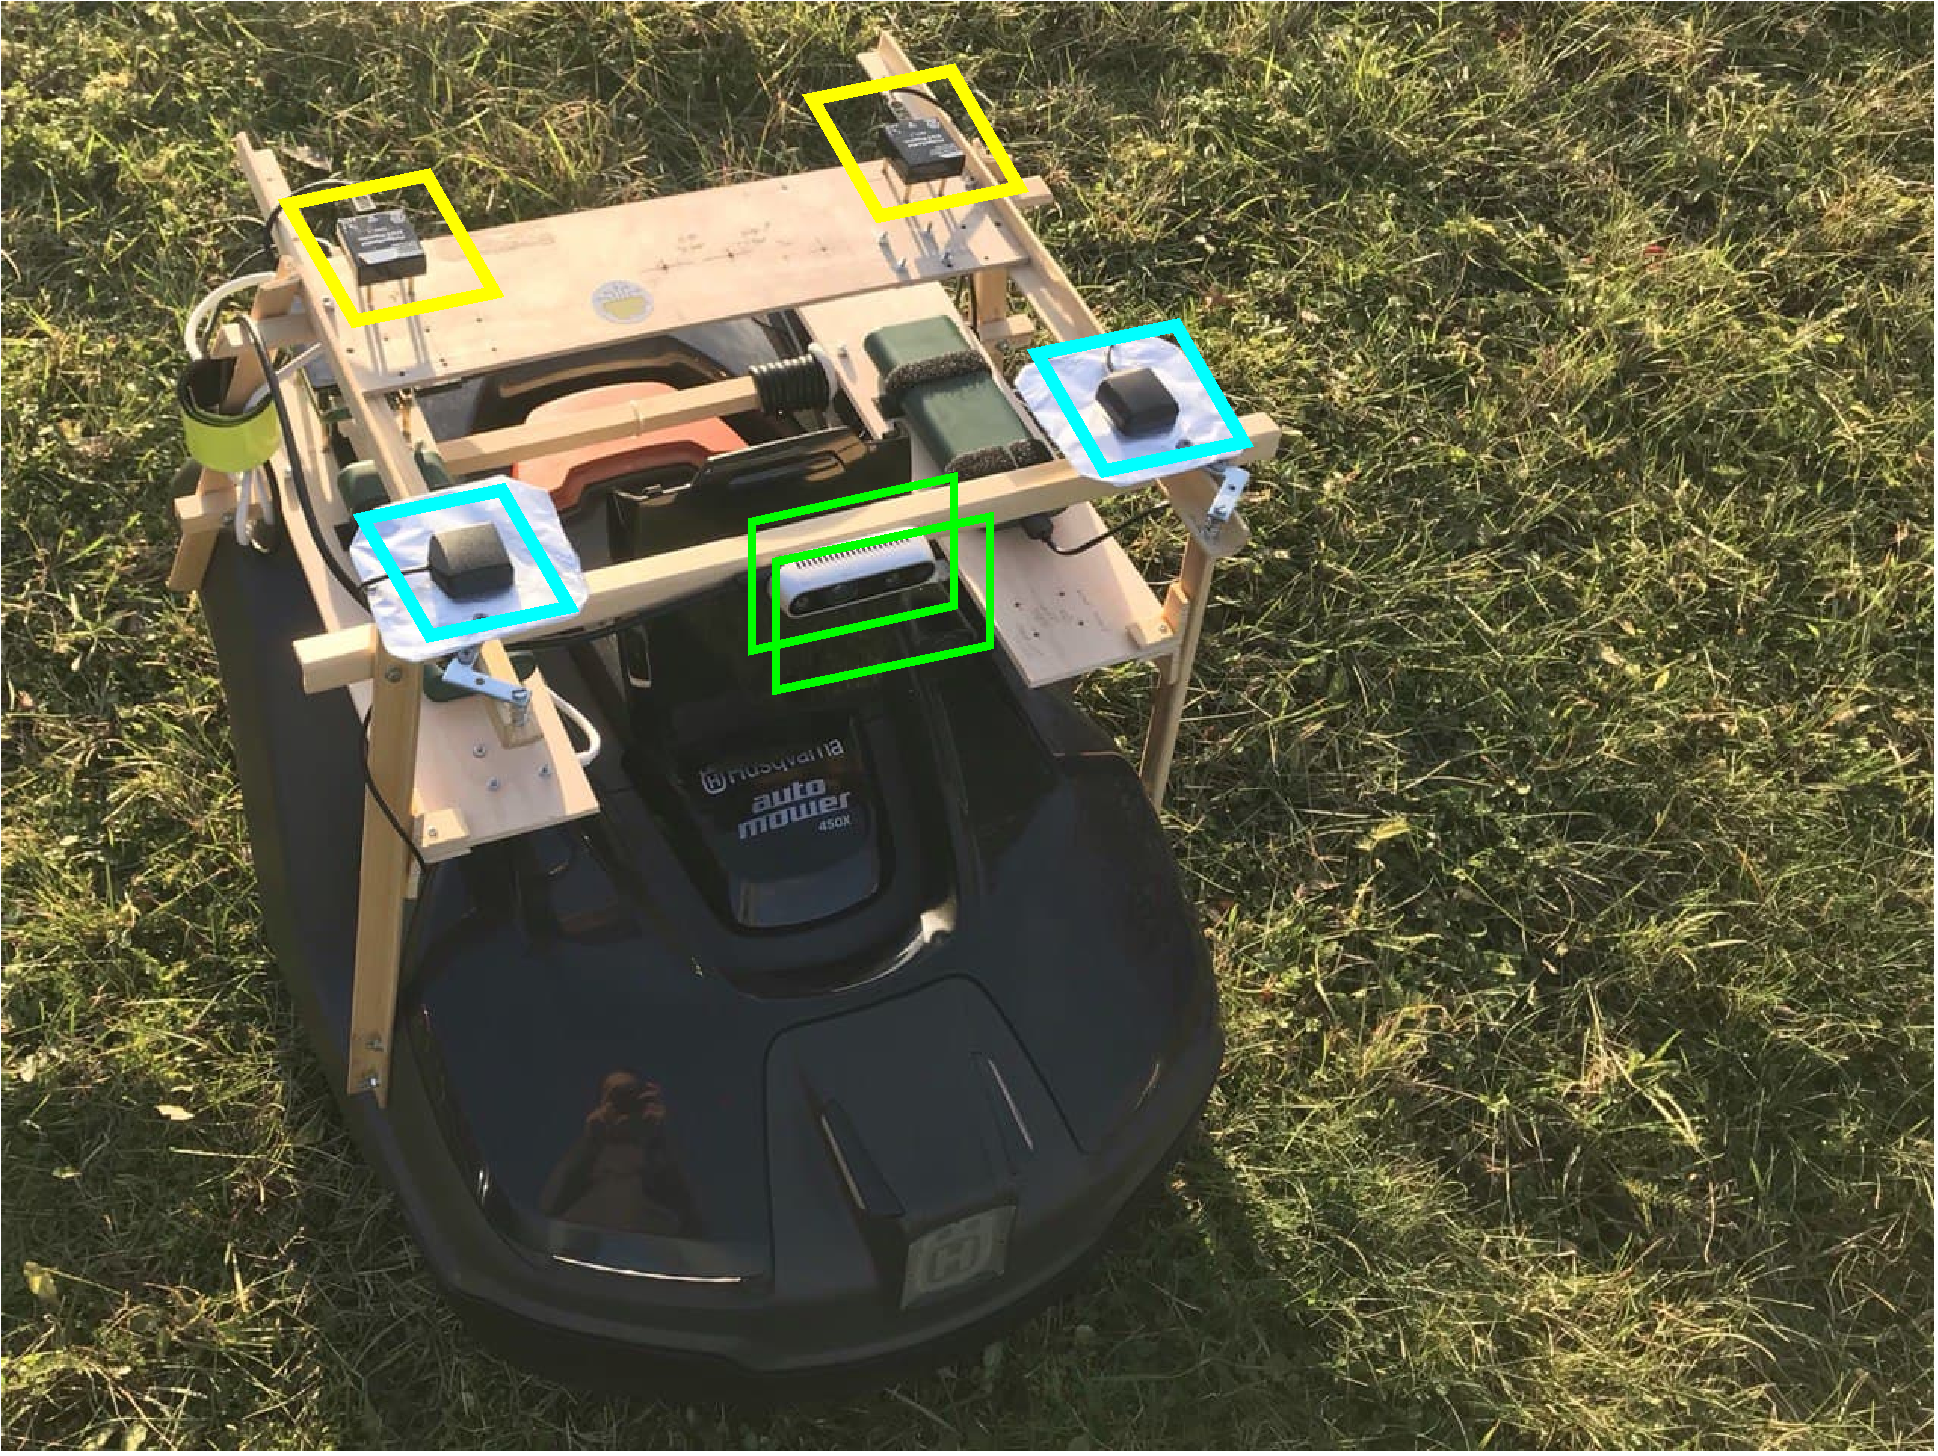
\includegraphics[clip, trim=0.5cm 0.6cm 8.5cm 0.6cm , width=0.45 \textwidth]{Images/1-Introduction/projectTheme.pdf}
		\caption{
			\gls{ALM} Model with focus on additional sensors:\\
			\glspl{IMU} [yellow], extra \gls{GNSS} receivers (not relevant) [cyan], and Camera [green].
			\centering }
		\label{fig:HardwareSetup}
	\end{center}
\end{figure}


\com{
\subsection{Scope}
Describe the boundary/limits of your thesis project and what you are explicitly not going to do. This will help you bound your efforts – as you have clearly defined what is out of the scope of this thesis project. Explain the delimitations. These are all the things that could affect the study if they were examined and included in the degree project.
\noindent
}

Since \glspl{ALM} are consumer products, some constraints will be taken into account. %, such as the configuration complexity and the sensors' cost analysis.
Those elements provide the rationale for this project to focus on some aspects rather than others.
Some of them are directly limiting and they are not going to be investigated further.
Some others instead will be included in the future works, discussed at the end of this thesis.
The most relevant are described below:
\begin{itemize}
    \item The operation area is projected into a \Gls{2D} environment. This allows for an initial definition for the localisation and mapping, and it could be expanded to \gls{3D} only after this phase has been refined.  
    \item The usage of an embedded device, such as a \gls{RPi}, limits the computational power of the module. Thus, the performance might not be as good as if a more powerful device would be used. %In this project, this aspect of optimization of the limited resources available on an embedded system will not be investigate.
    %\\~\\
    \item A complete \gls{SLAM} algorithm is too computationally expensive to perform well in real-time, considering the dynamic outdoor environment and the limited computational power.
    The proposed approach is to split the two different phases.
    The localisation aspect will be achieved with a sensor fusion approach. The mapping simply uses its resulting pose to update its map using eventual collision events.%receiving directly a predefined map layout configuration of the environment with a given starting point of the \gls{ALM} should ease the process of  within it.
    \item Relying on a camera in outdoor settings means that the weather conditions and time of mowing can affect the results.
    As such, the testing will be performed in similar configurations, and, if possible, with an attitude towards limiting this issue.
    \item A Range Finder Sensor, e.g., lidar, was not considered as most of the outdoor environment will be either sparse or empty.
    Thus, the sensor would not be able to provide valuable improvement to justify the expensive choice.
    Moreover, such a sensor requires a relevant amount of computational power to be run.
\end{itemize}


%The two additional \gls{GNSS} receivers have not been exploited as they provide poor performances.

\section{Hardware}
\label{sec:system}

\noindent
The proposed architecture is based on the \gls{HRP}, with its original board and sensors, with the addition of a Raspberry Pi 4, which provides higher computational performance, and additional sensors to capture additional phenomena used by the localisation module.
The proposed architecture is defined in Figure \ref{fig:hard-conf}.
%The original board is tasked to guide the \gls{ALM} and make him move according to the desired path, also at the end the \gls{ALM} was free to run its random path and use the algorithm implemented to stay inside the boundaries.


\begin{figure}[!ht]
	\begin{center}
		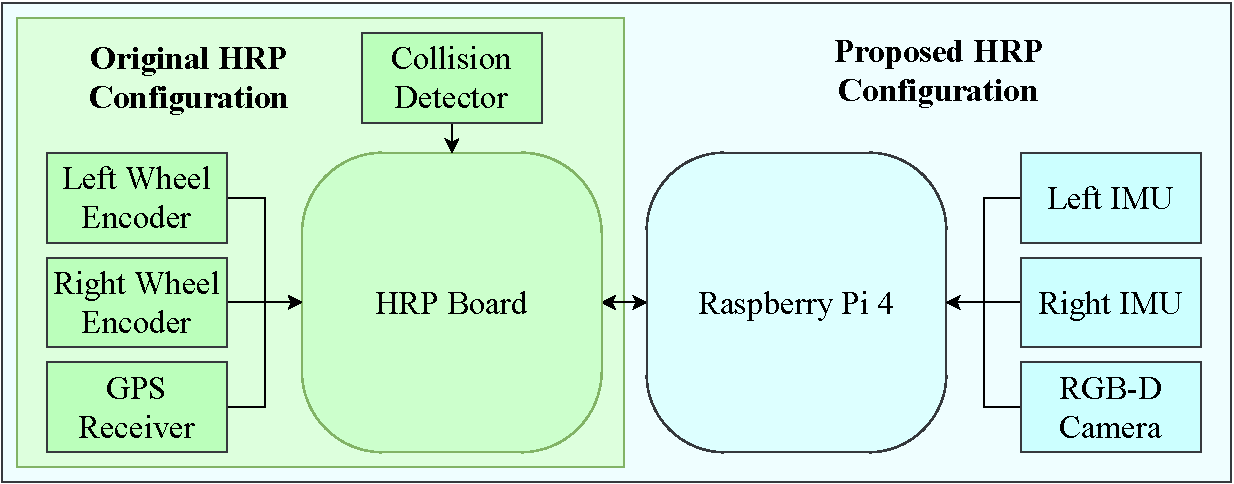
\includegraphics[width=1 \textwidth]{Images/3-0-SetUp/HWSetUp.pdf}
		\caption{Hardware Configuration including computational systems(rounded) and sensors(squared) of the original platform(green) with the updated version(blue). \centering }
		\label{fig:hard-conf}
	\end{center}
\end{figure}


%\subsection{HRP Board}
%\noindent 
The main board of the \gls{HRP} is a STM32-based microcontroller, shown in Figure \ref{fig:hrp-board}.
It is used to provide basic features for the \gls{ALM}, e.g., wheel control and collision detection. 
For the specific case of the \gls{HRP}, Husqvarna has provided an USB interface to connect it to external host computers, allowing for the connection with the Raspberry Pi 4 module.
\begin{figure}[!ht]
	\begin{center}
			\begin{center}
				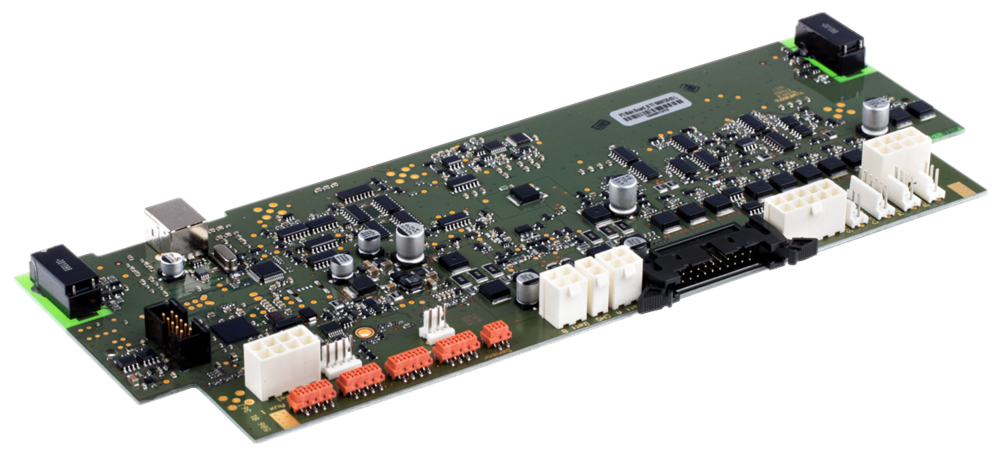
\includegraphics[width=0.5\textwidth]{Images/3-0-SetUp/586813503.png}
			\end{center}
			\caption{\gls{HRP} Main board.}
			\label{fig:hrp-board}
	\end{center}
\end{figure}

%\subsection{Raspberry Pi 4}
%\noindent 
The Raspberry Pi 4 Model B has been chosen as host computer, as shown in Figure \ref{fig:rpi4}.
It has been added to supplement the \gls{HRP} board, providing additional computational power for the implementation of additional features, i.e., the localisation and mapping modules. 
Moreover, additional hardware such as the \glspl{IMU}, and the \gls{RGBD} camera have been directly connected to it to improve the final \gls{HRP} configuration.
This platform is the one which will be used to guide the \gls{ALM}.
\begin{figure}[!ht]
	\begin{center}
			\begin{center}
				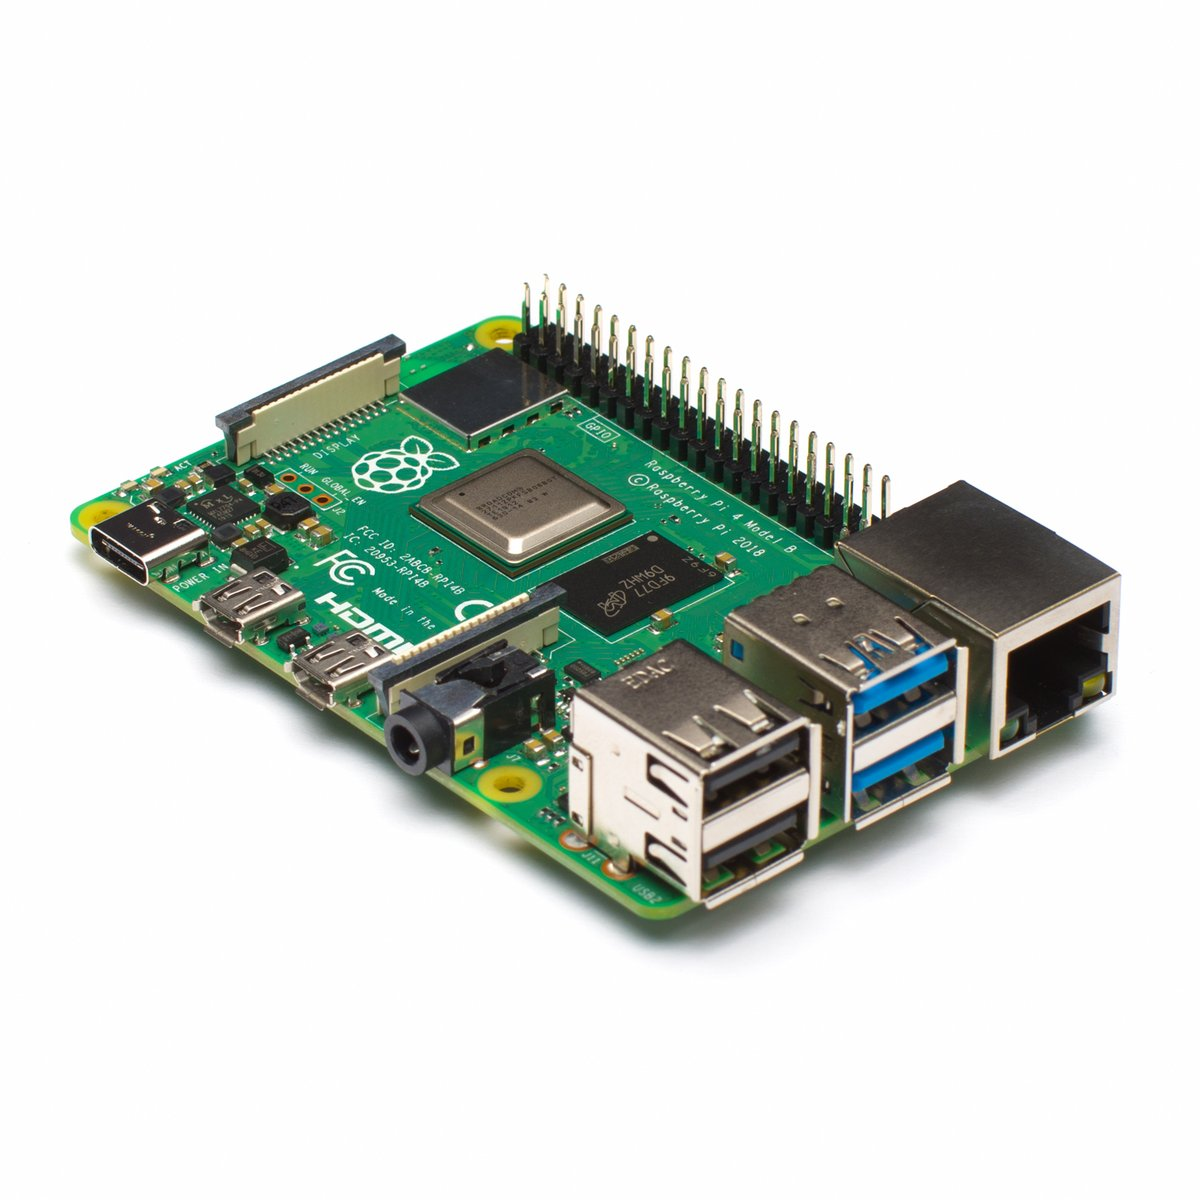
\includegraphics[clip, trim=2cm 8cm 2cm 10cm , width=0.5\textwidth]{Images/4-Methods/RPi4.jpg}
			\end{center}
			\caption{Raspberri Pi 4 Model B.}
			\label{fig:rpi4}
	\end{center}
\end{figure}

%\subsection{Wheel Encoders}
%\noindent
The wheel encoders are included in both of the motors of the wheels of the \gls{ALM}, inside the Motor Kit shown in Figure \ref{fig:wheel}.
They measure the wheel displacement and they provide \gls{WO} through estimates of the wheel velocities used to derive the related linear and angular velocities of the \gls{ALM}.
They work at a frequency of \SI{200}{Hz}.
\begin{figure}[!ht]
	\begin{center}
			\centering
			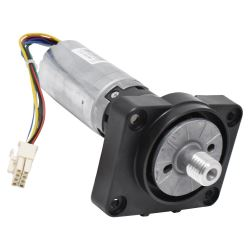
\includegraphics[width=0.30\textwidth]{Images/4-Methods/MotorEnc.jpeg}
			\caption{Motor Kit for Automower 450X.}
		\label{fig:wheel}
	\end{center}
\end{figure}


%\subsection{GPS Receiver}
%\noindent
A \gls{GPS} receiver is directly embedded in the automower as part of the Connect Kit developed by Husqvarna for positioning purposes, as shown in Figure \ref{fig:gps-module}.
It is available for the advanced \gls{ALM} model the \gls{HRP} is built upon and it is mounted on the center of the \gls{HRP}, as per assembly instructions.
Its full specifications have not been disclosed by the \gls{ALM} producer, but it can be said that it is a combined sensor with loosely coupled GNSS-INS integration, i.e., it uses both measurements from an internal \gls{IMU} sensor and the \gls{GPS} receiver to provide more reactive position fixes. 
Its measurements are derived using the computations of pseudoranges obtained from the \gls{GPS} receiver and fusing them with the measurements of an \gls{INS}, as such, consecutive measurements are correlated.
%TODO
% Better define the Loosely Coupled GNSS-INS Integration not disclosed by the \gls{ALM} producer
It works at a frequency of \SI{1}{Hz} and it is the only sensor which directly provides the measurements related to the pose states of position and orientation.
\begin{figure}[!ht]
	\begin{center}
			\begin{center}
				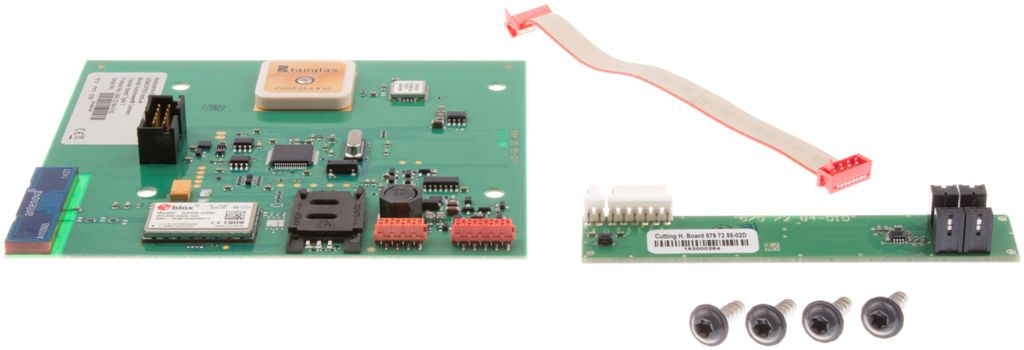
\includegraphics[width=0.75\textwidth]{Images/3-0-SetUp/Husqvarna_Automower_Connect_module_2.jpeg}
			\end{center}
			\caption{Husqvarna Automower Connect module.}
			\label{fig:gps-module}
	\end{center}
\end{figure}


%\subsection{IMUs}
%\noindent
The additional \glspl{IMU} adopted are the PhidgetSpatial Precision 3/3/3 High Resolution, shown in Figure \ref{fig:spatial}.
They are mounted on the structure of the \gls{HRP} in position [$x=0$\SI{}{cm}, $y=\pm16$\SI{}{cm}, $z= 37$\SI{}{cm}] and orientation [$\theta_z=0$\SI{}{rad}] with respect to the robot coordinate frame $P_R$.
They include gyroscopes, accelerometers, and compasses on each of the 3-axis.
The measurements of angular velocity and linear acceleration are used, respectively, to improve the orientation estimates and to model the noise of the prediction step.
It provides angular velocity and linear acceleration at a frequency of \SI{250}{Hz}.
\begin{figure}[!ht]
	\begin{center}
			\begin{center}
				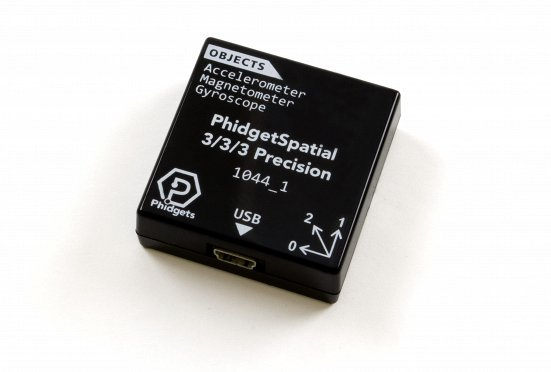
\includegraphics[width=0.5\textwidth]{Images/4-Methods/1044_1B.jpg}
			\end{center}
			\caption{IMU Sensor.}
			\label{fig:spatial}
	\end{center}
\end{figure}



%\subsection{RGB-D Camera}
%\noindent 
The device adopted is the Intel® RealSense™ depth camera D435, shown in Figure \ref{fig:camera_sensor}.
It is mounted on the structure of the \gls{HRP} in position [$x=0.23$\SI{}{cm}, $y=0$\SI{}{cm}, $z= 33$\SI{}{cm}] and orientation [$\theta_z=0$\SI{}{rad}] with respect to the robot coordinate frame $P_R$.
It provides \gls{RGBD} images through a stereo camera, i.e., both \gls{RGB} and Depth information.
The images it provides are used to generate the \gls{VO} estimates, bases on the displacements of features identified in consecutive shots.
It is used to provide velocity measurements through \gls{VO} at a frequency of \SI{5}{Hz}.
\begin{figure}[!ht]
	\begin{center}
			\begin{center}
				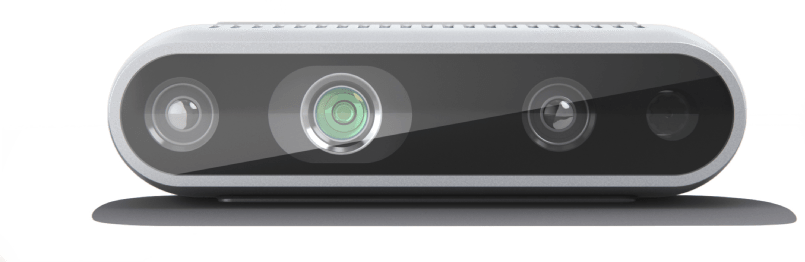
\includegraphics[width=0.5\textwidth]{Images/4-Methods/d435i-1.png}
			\end{center}
		\caption{Camera.}
		\label{fig:camera_sensor}
	\end{center}
\end{figure}


%\subsection{Collision Sensors}
%\noindent
The collision sensors, one of which is shown in Figure \ref{fig:collision_sensor}, detect when the frame of the automower has been in contact with an object.
They fire an event whenever the external frame bumps with an object and consequently reach the touch sensors positioned on the back of the wheels.
Thus, they allow for the detection of the objects and they are used to update the knowledge of the map.
\begin{figure}[!ht]
	\begin{center}
			\begin{center}
				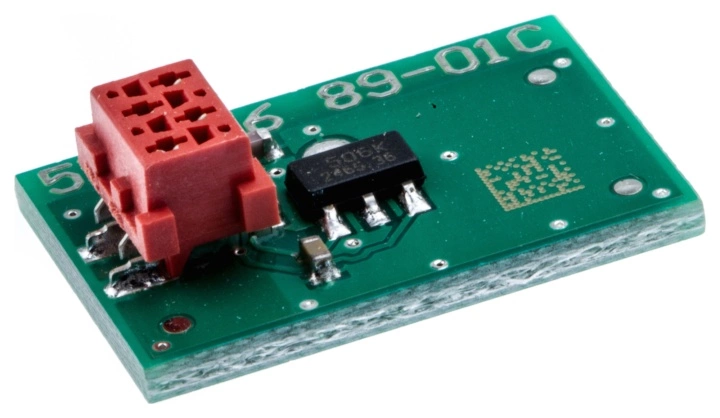
\includegraphics[width=0.5\textwidth]{Images/3-0-SetUp/Collision.png}
			\end{center}
		\caption{Circuit board collision sensor.}
		\label{fig:collision_sensor}
	\end{center}
\end{figure}


\section{Software}
\label{sec:soft-system}
\noindent The following software modules are adopted to code the required features.

As the \gls{HRP} is a \gls{ROS}-enabled platform, its latest available version has been used, namely, ROS Noetic.
For its installation, the Ubuntu operating system 20.04 has been choosen for the Raspberry Pi 4, instead the \gls{HRP} board runs a proprietary software which is not disclosed, but its program modules are written in C++ and they interface with ROS.
The software languages which have been used are C++11 for both the internal software and the hardware related tasks, such as the controller of the \gls{HRP} and the sensor's drivers.
Python 3.8 has been chosen for the high level tasks identified, such as the localisation and mapping modules developed as main contributions.
The different software modules are structured using \gls{ROS} nodes, which are sharing data using specific \gls{ROS} topics. An overview of the \gls{ROS} framework is available in Appendix \ref{ch:ros}. 

\cleardoublepage
    
    \chapter{Method}
\label{ch:methods}

\noindent In this chapter, the contributions proposed and applied during this thesis are discussed.
The proposed architecture defined in Chapter \ref{ch:setup} is shown.
Afterwards, the experiment configuration is described.% to show how the proposed methodology addresses the research goals.
Finally, the localisation and mapping models are presented, along with their respective evaluation techniques.

\section{Proposed Architecture} 
\label{ch:prop-architecture}
\noindent The proposed architecture for the final system is shown in Figure \ref{fig:arch-structure}. 
The localisation module is defined using a sensor fusion filter.
%This approach exploits available measurements, hence limiting the drawbacks of individual sensors and highlighting their contributions.
The proposed approach is an \gls{EKF}, chosen due to its robust and adaptable nature.
The \gls{EKF} enables for fast and reliable fusion of heterogeneous sensors in a way that allows the \gls{ALM} to have a real-time and accurate estimate of its pose.
The mapping module is defined using the results of the localisation as a baseline, and exploiting the collision detection measurements of the \gls{ALM}.
Through the use of these components, a virtual boundary is created and the presence of objects within it will be provided by the events fired by the collision sensors.
%Finally, the methodology adopted to evaluate the performances of these modules is defined. \{where is this defined? Maybe cut this sentence}
\begin{figure}[H]
	\begin{center}
	\centering
		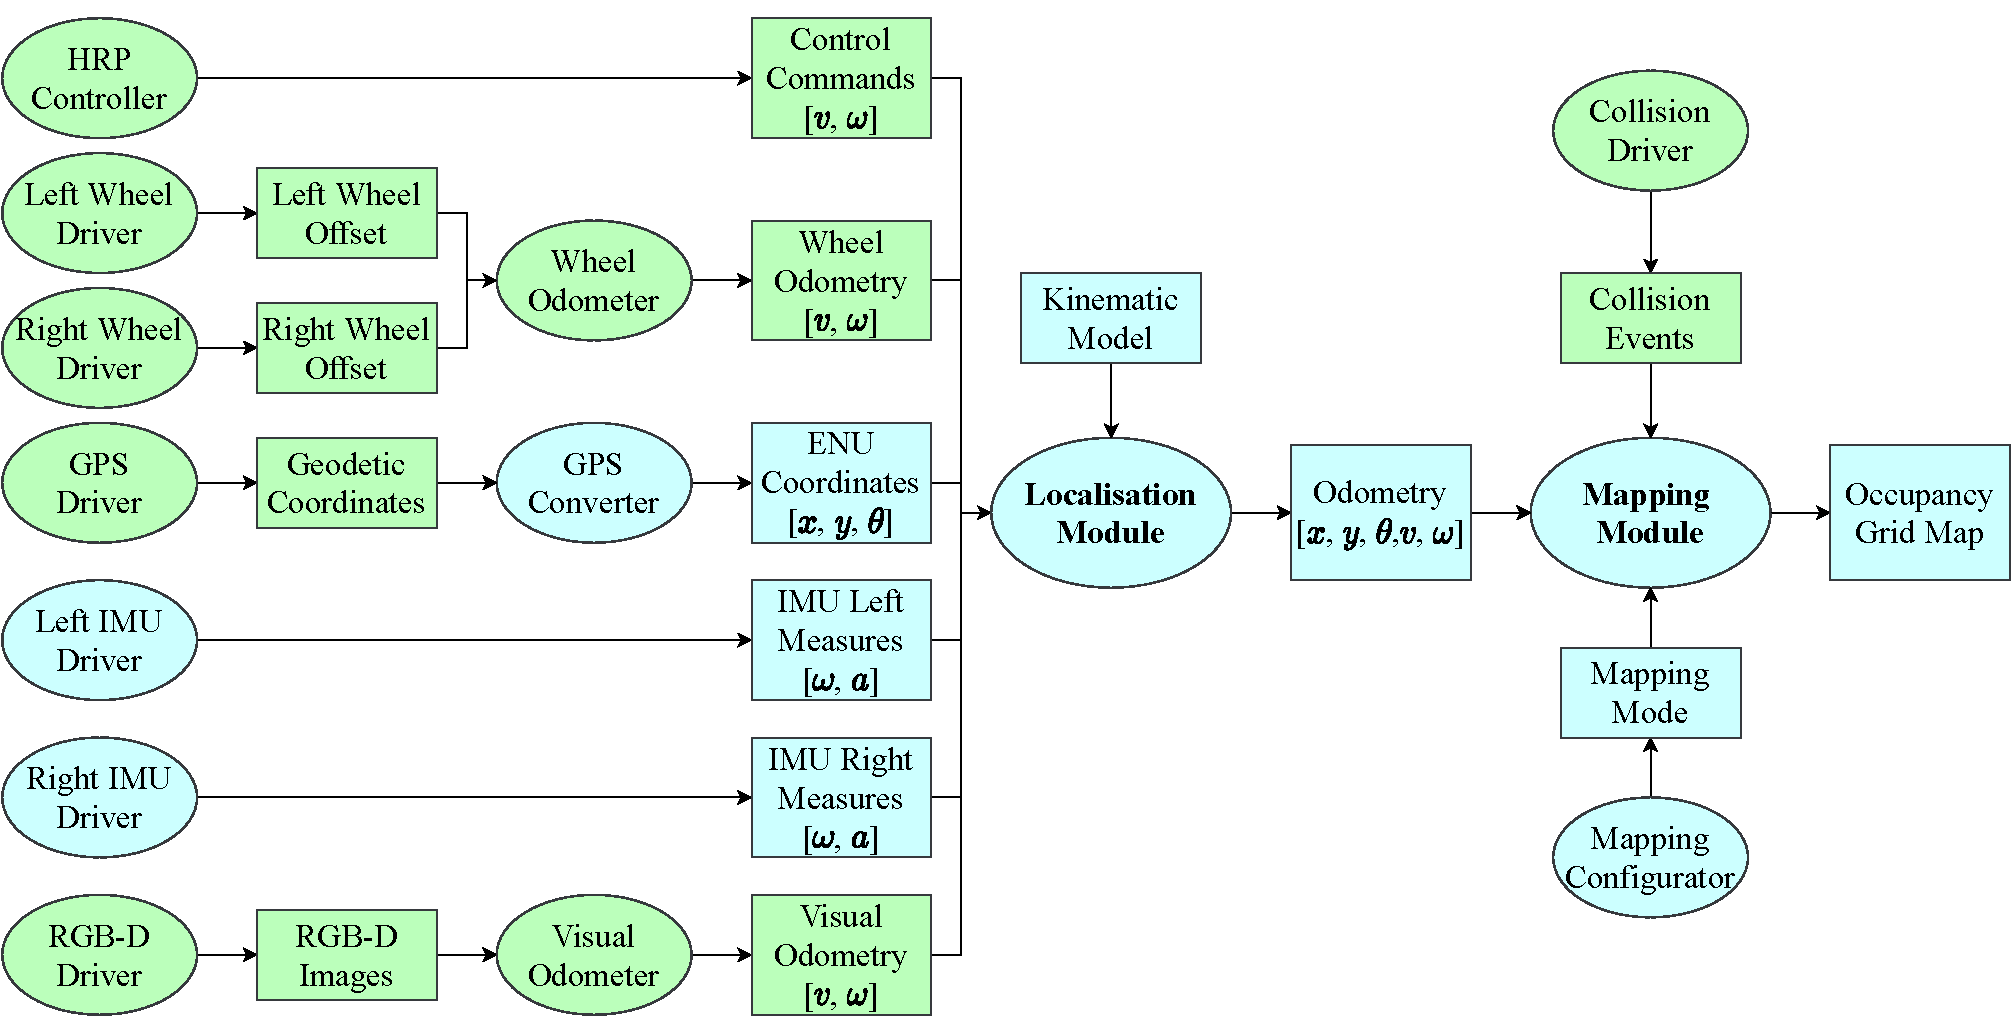
\includegraphics[width=1\textwidth]{Images/3-0-SetUp/SWSetUp.pdf}
		\caption{Software nodes(ellipses) and data structures(rectagles) including\\
		both available(green) and newly developed(blue) components.\\
		In bold the main contributions.\centering }
		\label{fig:arch-structure}
	\end{center}
\end{figure}
\section{Experiments}
\noindent The proposed architecture will be evaluated using multiple experiments, in which the \gls{ALM} is teleoperated by an external computer interacting with the \gls{HRP} Controller.
It sets the control commands as the linear and angular velocities, as defined during the kinematic analysis in Section \ref{ssec:kin_a}.

Some initial training tests are run to check the system's integrity and the correct interaction of the modules.
The data gathered in these multiple outdoor runs is then used to test and analyse the performance of the system.
Some tests have been made to define the calibration of the sensors against a ground truth identified using measure tape.
Other runs checked an accurate system's behaviour while steering.
Final tests ensured that the collision events are estimated with a certain degree of precision.

After this first phase, the proposed system's architecture is analysed with a testing run on gravel and a validation run on grass.
Each experiment will consist of both the localisation and mapping modules.
%Regarding the localisation topic, the experiments will be evaluated using different sensors' configurations.
The evaluation of the different sensors' configurations are performed in a successive phase of the experiment.
During the outdoor runs, the input measurements from the sensors are registered.
In a second moment, the results are replayed to compute the system's performance and to analyse which of their possible configurations provided the best results.
%The analysis will be conducted separately for the modules and their related evaluation metrics used for each respective component are described in the following sections. 

The results are considered valid if they show that the same methodology adopted provides similar results in different settings.
The methodology adopted during the training of the filter is then tested in the validation experiment to ensure that the performances are indifferent to the environment.
%The method is valid if the simulation filtering provide values close to the ground truth with the same configuration.%, showing that if the assumptions are validated then the system behaves as best estimator.


\subsection{Gravel Testing Experiment}
\noindent
The testing experiment has been run on a parking lot with gravel floor.
It has been used to test the first complete configuration of the \gls{ALM}.
In this case, only the boundary setting on the mapping module has been implemented.

\subsection{Grass Validation Experiment}
\noindent
The final validation has been made on a park with tall grass to test a more realistic scenario.
The sensor fusion localisation and the occupancy grid mapping have been run together using the findings of the gravel test.
Furthermore, the complete mapping module has been adopted. 

\subsection{Ground Truth Generation}
\label{sec:gt}
\noindent The ground truth is constructed manually by checking the actual path travelled by the robot with the usage of a measure tape properly set during the experiments.
The values obtained are then used to generate a dynamic virtual run which follows the real run as it was carried out in reality, which is finally adopted to check the system's performance.

\section{Localisation}
\label{sec:loc-method}
\noindent The Localisation Module is based on a \gls{EKF} which unifies and fuses the information derived by the kinematic model, the control commands, and the sensors' measurements.
It has been selected and adopted for its time performances and reliability.
As analysed in~\cite{801027}, the performance of a \glspl{KF} driven by the kinematic model are similar to the one obtained by a filter driven by the \gls{WO} measurements.
However, as in this project the control commands are also available, the Prediction phase is defined by the kinematic model while the \gls{WO} measurements are used by the \gls{EKF} for the Correction phase.

The filter works with a discretised time system which is executed with a frequency of \SI{250}{Hz}, which is the highest sampling frequency among the sensors, obtained by the \glspl{IMU}.
%It improves the \gls{KF} allowing for the management of non-linear systems and the possibility to account for dynamic sensors' noise.
At first, the Prediction step is computed, using the sampling period, while the system gathers new sensors' measurements, which are used to dynamically create the components for the Correction step. 
After a delay has been waited to reach the desired frequency rate, the Correction step merges the measurements into the filtered state and covariance before reiterating this procedure. 
%Check
The execution of the steps is not immediate, as it needs some time consuming computations, so the sampling rate of the \gls{EKF} is variable and the related time step is defined dynamically by the varying $\boldsymbol \Delta_t$.
The algorithm will use this varying sampling period at each prediction step to accurately transition the filtered estimate into the discretised predicted estimate defined by this value. 

\subsection{Calibration Step}
\noindent
Before starting to fuse the data for the sensors, an initial phase of calibration for some sensors is necessary.
In this preliminary step, the measurements obtained from some sensors are used to elaborate a value that will be later adopted in their covariance measurement matrices $R_*$, used to weight the relevance of their measurements in the correction phase. %provide on their own the variance of all their estimates.
This step is needed to ensure that the \gls{EKF} will behave properly in different ground conditions.

This operation is needed by the wheel encoders and by the \gls{GPS} receiver as their variances are not disclosed.
The calibration of the GPS receiver is derived after five minutes of stationary state.
During this period, the provided \gls{HDOP} error rate, which is obtained internally using the pseudoranges measurements, is scaled to match the variances estimated from its initial fix in the local frame. 
This scaling value is then used throughout the entire test to adapt the varying \gls{DOP} estimate into a varying \gls{GPS} measurement covariance matrix.
The position estimates derived from this still pose are also averaged to provide the initial reference fix adopted by the \gls{GPS} measurement model to compute its local position.
The wheel encoders compute their variances using the measurements obtained by moving the \gls{ALM} in a sample run of \SI{5}{meters} before the test. 
The obtained calibration variances are adopted by the wheel encoder measurement covariance matrix.
The initial calibration run is also exploited by the \gls{GPS} measurement model used to compute the variance of the orientation estimates obtained as defined in \ref{sec:gps-rec-mod}.


\subsection{Prediction Model}

\noindent The prediction phase is driven by the kinematic model and the eventual control commands, as defined in Figure \ref{fig:TikzKine}.
It has been adopted given its better performance with respect to the odometer driven model~\cite{801027}.

After the calibration phase, the \gls{ALM} is in a stationary state.
The system will then start with all its state variables $\mathbf{X}_0^-$ set to $0$.
The initial Covariance matrix $P_0$ is set as the identity matrix multiplied by $1^{-3}$.

The state variables needed to provide the most accurate positioning in a \gls{2D} environment are defined in \eqref{eq:state-transf}:
\begin{equation}
	\label{eq:state-transf}
	\mathbf{X}_t =
	\begin{bmatrix}
		\mathbf{x}_t & \mathbf{y}_t & \boldsymbol \theta_t & \mathbf{v}_t & \boldsymbol \omega_t
	\end{bmatrix} ^T
\end{equation}
From the definition of the Kinematic Model in Figure \ref{fig:TikzKine}, the first three positional elements, i.e., $\mathbf{x}_t$, $\mathbf{y}_t$, and $\boldsymbol \theta_t$, are related to the global frame. 
Instead the following inertial elements, i.e., $\mathbf{v}_t$ and $\boldsymbol \omega_t$ are defined from the robot frame.
As assumption, the system will start with a known initial state $\mathbf{X}_0$ of mean $0$ for each element, and it will follow a Constant Velocity model.

%\subsubsection{Transition}
The transition matrix related to the states defined in Equation \eqref{eq:state-transf} and to the kinematic model of Figure \ref{fig:TikzKine} is presented below:
\begin{equation}
	\label{eq:trans-mat}
	A_t
	=
	\begin{bmatrix}
		1 & 0 & 0 & \cos(\boldsymbol \theta_t) \cdot \Delta_t & 0 \\
		0 & 1 & 0 & \sin(\boldsymbol \theta_t) \cdot \Delta_t & 0 \\
		0 & 0 & 1 & 0 & \Delta_t  \\
		0 & 0 & 0 & 1 & 0 \\
		0 & 0 & 0 & 0 & 1 & 
	\end{bmatrix}
\end{equation}
where $\boldsymbol \theta_t$ is the orientation value of the current state and $\boldsymbol \Delta_t$ is the current sampling period used by the \gls{EKF} for the discretisation.
This model accounts for the transformation of the linear velocity and angular velocity to update the pose states defined in \eqref{eq:dof}.

%\subsubsection{Control}
As defined in Section \ref{ssec:kin_a}, the \gls{ALM} is controlled using the linear and angular velocities.
This configuration is used by the \gls{EKF} to complete the Prediction step using the following Control matrix $B$ and control state $\mathbf{u}_t$, as in:% Equations \eqref{eq:cmd}.
\begin{align}
	\label{eq:cmd}
	B &=
	\begin{bmatrix}
		0 & 0 \\
		0 & 0\\
		0 & 0\\
		s & 0\\
		0 & s
	\end{bmatrix}
	&
	\mathbf{u}_t &=
	\begin{bmatrix}
		\mathbf{v} - \mathbf{v}_t  \\
		\boldsymbol \omega - \boldsymbol \omega_t \\[0.3em]
	\end{bmatrix}
\end{align}
where $s$ is a smoothing factor adopted to make the transition from command received to actuation more realistic. %and  $\Delta_t$ is the varying time step of the \gls{EKF}, to dynamically define the matrix. 
%This smoothing matrix $B$ is adopted to avoid reaching the desired velocities sent to the robot , i.e., $\mathbf{v}$ and  $\boldsymbol \omega$. % obtained by a specific topic. 
%TODO Check
The control state $\mathbf{u}_t$ is defined as the difference between the control velocities desired, $\mathbf{v}$ and  $\boldsymbol \omega$, and the estimated velocities from the related state of $\mathbf{X}_t$.
This formulation enables the estimate to converge to the desired velocities in a time period defined by $F$, for which the chosen value for $s$ is set at each step as the value of the sampling period indicating that the filter will take indicatively a whole second to reach the desired velocities. %to ensure that including the control then the estimate will follow the desired value in the number of seconds defined by $F$.
\com{
	and $\mathbf{s}_{i}$ is used to make the transition from command received and actual actuation more smooth by limiting the innovation given by the respective control through a scaling value equal to the frequency of the system: $\mathbf{s}_i = \frac{1}{Hz}$, with $Hz$ as the frequency of the \gls{EKF}.
}

%\subsubsection{Uncertainty}
\com{
	The noise vector related to the state variables estimate is adaptively defined by $\boldsymbol \eta$ as in \eqref{eq:noise-p}.
	\begin{equation}
		\label{eq:noise-p}
		\boldsymbol \eta
		=
		\begin{bmatrix}
			\boldsymbol \eta_{\mathbf{x}}  &
			\boldsymbol \eta_{\mathbf{y}} &
			\boldsymbol \eta_{\boldsymbol \theta}  &
			\boldsymbol \eta_{\mathbf{v}} &
			\boldsymbol \eta_{\boldsymbol \omega} &
			\boldsymbol \eta_{\mathbf{a}}
		\end{bmatrix} ^T
	\end{equation}
	where $\eta_i \sim \mathcal{N}(\mu_i,\,\sigma_{ii}^{2})$ with $\mu_i = 0$, $\sigma_{ii}^2 = 0.1$, and $ i = \{ \mathbf{x} , \mathbf{y} , \boldsymbol \theta , \mathbf{v} , \boldsymbol \omega , \mathbf{a} \}$
	where $\sigma_{\mathbf{xx}}^2 = \sigma_{\mathbf{yy}}^2 = \sigma_{\mathbf{\boldsymbol \theta \boldsymbol \theta}}^2  = \cfrac{{\boldsymbol \Delta_t}^2}{2}$, and $\boldsymbol \Delta_t$ is the time step used by the \gls{EKF}.
}

The prediction of the estimate regarding the state variables is defined in the \gls{KF} by equations \eqref{eq:pred-state-formula} and \eqref{eq:pred-state-formula-noc}, depending on the chosen configuration:
	\begin{align}
		\label{eq:pred-state-formula}
		\hat{\mathbf{X}}_{t+1}^-& = A \cdot \mathbf{X}_t^- + B \cdot \mathbf{u}_t && \text{when control is considered} \\
		\label{eq:pred-state-formula-noc}
		\hat{\mathbf{X}}_{t+1}^- & = A \cdot \mathbf{X}_t^- &&       \text{when control is not considered} 
	\end{align}

%\subsubsection{Linearisation}

As the \gls{KF} is not able to deal with non-linear systems, the Jacobian of the Transition matrix $A$ must be obtained to linearise the non-linear equations with a first-order Taylor expansion.
The resulting matrix $J_A$, defined in \eqref{eq:j-a}, can then be used by the \gls{EKF} for the prediction of the Covariance matrix:
\begin{equation}
	\label{eq:j-a}
	J_A
	=
	\begin{bmatrix}
		1 & 0 & -\sin(\boldsymbol \theta_t) \cdot \Delta_t & \cos(\boldsymbol \theta_t) \cdot \Delta_t & 0  \\
		0 & 1 & ~\cos(\boldsymbol \theta_t) \cdot \Delta_t & \sin(\boldsymbol \theta_t) \cdot \Delta_t &  0  \\
		0 & 0 & 1 & 0 & \Delta_t \\
		0 & 0 & 0 & 1 & 0  \\
		0 & 0 & 0 & 0 & 1  
	\end{bmatrix}
\end{equation}
where $\boldsymbol \theta_t$ is the current orientation value of the system, which is here used to linearise the non-linear system.


The noise matrix $Q$ is defined by uncorrelated and zero-mean white noise $q_t$, with its elements set dynamically as the related noise of the state velocities.
The adopted matrix formulation is defined by an adaptive approach in which the noise values are directly related to the acceleration the system is subject to. %,  the error in the process as a function of the acceleration.
The definition of two variables, $q_v$ and $q_{\omega}$, is needed to model this dynamic matrix, as the linear and angular accelerations of the robot respectively.
They are obtained using the acceleration measurements estimated by the \glspl{IMU} (using \SI{9.81}{\metre\per\square\second} as default is a good estimate in absence of those sensors, as experimented by~\cite{king_low_2008}) and exploiting their positions of the \glspl{IMU} on the robot, i.e., parallel on the $Y$ axis with equal displacement $d_{IMU}=\SI{16}{cm}$, and some basic rotational kinematics formula~\cite{rotational} defined as:% \eqref{eq:rot}:
\begin{align}
    q_v = \cfrac{a_L + a_R}{2} &&
    q_{\omega} = \cfrac{a_L - a_R}{2 \cdot d_{IMU}}
    \label{eq:rot}
\end{align}
where $a_L$ and $a_R$ are the linear acceleration measurements provided by the \glspl{IMU} positioned respectively on the left and right side of the \gls{ALM}, with the distance from the rotation center defined by $d_{IMU}$. 
The Jacobian of matrix $C$, i.e., $J_C$, is used to account for both the non-linearities of the system and their relation to the time delay of the prediction phase.
It is adopted to model the matrix of covariance of process noise $Q$, defined by the acceleration values obtained above.
\begin{align}%Continuous White Noise Model
	\label{eq:q-p}
	J_C
	=
	\begin{bmatrix}
		-\sin(\theta) \cdot \frac{\boldsymbol \Delta_t^2}{2}  & 0 \\
		\cos(\theta) \cdot \frac{\boldsymbol \Delta_t^2}{2}  & 0 \\
		0 & \frac{\boldsymbol \Delta_t^2}{2} \\
		\Delta_t & 0 \\
		0 & \Delta_t
	\end{bmatrix}
	&&
	Q
	=
	\begin{bmatrix}
		q_v & 0 \\
		0 & q_{\omega}
	\end{bmatrix}
\end{align}
where $\boldsymbol \Delta_t$ is the sampling period for the current \gls{EKF} prediction step.
This formulation is defined to ensure that with high acceleration measurements, the system will be characterised by an higher uncertainty and the importance given to the measurements will be more higher in the correction step. % Wiener

\com{
The diagonal assumption means that the errors between variables are not directly associated, but their relationships and related propagation of errors will appear through the transition matrix Jacobian  $J_A$~\cite{king_low_2008}.
}

Finally, the predicted covariance matrix, defined by $\hat{P}_{t+1}$ is updated during the prediction using the Jacobian $J_A$ and the process noise covariance $Q$ modelled by $J_C$. %, as in Equation \eqref{eq:cov-p}.
\begin{align}
	\label{eq:cov-p}
	%P_0 &= I \cdot 1^{-3} &
	\hat{P}_{t+1} & = J_A \cdot P_t \cdot J_A^T + J_C \cdot Q \cdot J_C^T
\end{align}%P_{p} & =  \frac{P_{p} +  P_{p}^T}{2} && \text{To ensure symmetry}


\subsection{Wheel Encoder Model}

\noindent
Through the wheel encoders attached to both wheels, an estimated velocity for them is calculated and used to determine its pose.
%This open-loop technique to determine the position and orientation is called \gls{DR}, as the new pose is estimated by using the last known pose and the new speed measurements.
The wheel encoders attached on each wheel provide an estimate of the number of pulses they detected. These encoder pulses need to be translated to an approximated wheel displacement through the transformation constant $C_{D}$ which is used to transform the number of pulses into meters:% provided by equation \ref{eq:wheel_meter}.
\begin{equation}
C_{D} = \frac{\pi \cdot W_D }{P_T}
\label{eq:wheel_meter}
\end{equation} where $W_D$ is the length of the wheel diameter in meters and $P_T$ is the number of pulses required to complete a wheel turn and it is specific for the wheel encoder placement.
This value is used to derive the velocity of each wheel separately, $\dot \delta_L$ and $\dot \delta_R$ as in:
\begin{equation}
\dot \delta_{L} = \frac{C_D \cdot E_L}{E_T}  \qquad
\dot \delta_{R} = \frac{C_D \cdot E_R}{E_T}
\label{eq:wheel_disp}
\end{equation}
where $E_L$ and $E_R$ the number of identified encoder pulses for the left and right wheels respectively, and $E_T$ is the encoder time resolution in seconds, given by its \SI{200}{Hz} sampling frequency.

Using these single wheel displacements, it is possible to calculate the linear velocity along the $x$ axis, $v$, and the angular velocity on the $z$ axis, $\omega$, with respect to the mobile robot frame using equations \eqref{eq:omega} and  \eqref{eq:vel} derived from the kinematics analysis.
\com{\begin{equation}
    \mathbf{v}_t  =\frac{\dot \delta_{R} + \dot \delta_{L} }{2} \qquad 
    \boldsymbol \omega_t = \frac{\dot \delta _{R} - \dot \delta_{L}}{B_W}
\label{eq:disp}
\end{equation} where $B_W$ is the length of the base width of the back wheel axis in meters.
}

\com{
These forward kinematics equations of this differential drive mobile robot are used to update the pose of the mobile robot, from time $t$ after a time step $\Delta_t$ to time $t+1$, in the global coordinate frame with the Euler first-order differential approximation~\cite{braun_first-order_1993}, as shown in equation \eqref{eq:eulerWheel}:
\begin{equation}
\begin{bmatrix} x_{t + 1} \\ y_{t + 1} \\ \theta _{t + 1} ~ \end{bmatrix}
=
\begin{bmatrix} {x_t} \\ {y_t} \\ {\theta _t}  \end{bmatrix}
+
\begin{bmatrix}  \cos (\theta _t ) & 0\\  \sin (\theta _t ) & 0 \\ 0 & 1 \end{bmatrix}
\cdot
\begin{bmatrix} \mathbf{v}_t  \\ \boldsymbol \omega_t \end{bmatrix} \cdot
\Delta_t
\label{eq:eulerWheel}
\end{equation}


This method is the one adopted by the original \gls{HRP} configuration to estimate its odometry, but it is subject to multiple errors and inaccuracies, as both the measurements and time delays will never be perfect.
%The systematic errors can be given by imperfectness of robot model as impreciseness in the wheel diameters or wheel base measures, which are used to estimate the movements.
%However, t
The presence of non-systematic random errors as result of usage of imperfect measurements are more difficult to model, e.g., wheel slippage, uneven terrain, and external forces applied.
The accumulative characteristic of these errors will break the stability of the system, making the estimate to drift after a period of time.
These conditions render this \gls{DR} model not adequate to determine the pose of the mobile robot, but the estimates provided by it could be still used to improve the positioning system, especially if corrected by an absolute position sensor, e.g., \gls{GNSS}.
}
\com{
\begin{align}
\mathbf{v}_{WO_t} & = \mathbf{v} &
\boldsymbol \omega_{WO_t} & = \boldsymbol \omega
\end{align}
}

The Measurement vector, $Z$, with its related Uncertainty vector, $R$, as used in the Correction step, are defined by equation \eqref{eq:meas-wheel} as follows:  
\begin{align}
\label{eq:meas-wheel}
\mathbf{Z}
=
\begin{bmatrix}
\mathbf{v}_t \\
\boldsymbol \omega_{t}
\end{bmatrix}^T
& \quad
\mathbf{R}
=
\begin{bmatrix}
\mathbf{r}_{\mathbf{v}_{t}} & 0\\
0 & \mathbf{r}_{\boldsymbol \omega_t}
\end{bmatrix}
\end{align}
where $\mathbf{r}_{\mathbf{v}_{t}}$ and $\mathbf{r}_{\boldsymbol \omega_t}$ are experimentally derived during the initial calibration phase.

The Measurement matrix, $H$, and its related Jacobian matrix, $J_H$, are defined by the following matrix, indicating that only the linear and angular velocities need to be fused:
\begin{equation}
H = J_H =
\begin{bmatrix}
0 & 0 & 0 & 1 & 0 \\
0 & 0 & 0 & 0 & 1
\end{bmatrix}
\end{equation}


\subsection{\gls{GPS} Receiver Model}
\label{sec:gps-rec-mod}
\noindent The embedded \gls{GPS} sensor estimates its global position by trilaterating the difference in received signals from multiple satellites. % the satellites' positions and trilaterating its  to estimate its absolute position global values in the global coordinate frame.
It provides measurements about its position in the global Earth-Centered, Earth-Fixed terrestrial reference system.
These values are then used to compute the difference from the initial starting point obtained through the initial calibration to find the offset position.
These values are then transformed into the local frame using the formulations specified in Appendix \ref{ch:conv-gnss} and they can be used by the sensor fusion algorithm.
The formulas adopted are: %used to obtain the distance between this mean value and the current value of the \gls{GPS} measurements is defined below, as the local difference from the initially obtained coordinate:
\begin{align}
\mathbf{x}_{GPS_t} & = \text{geodetic2enu}( lat_t - lat_{ref})\\
\mathbf{y}_{GPS_t} & = \text{geodetic2enu}( long_t - lon_{ref})
\end{align}
where $lat_t$ and $long_t$ are, respectively, the current estimates in the global frame in latitude and longitude,  while $lat_{ref}$ and $long_{ref}$. 

The measurement vector, $Z$, with its related uncertainty vector, $R$, as used in the Correction step, are defined by equation \eqref{eq:meas-gps} as follows:  
\begin{align}
\label{eq:meas-gps}
\mathbf{Z}
=
\begin{bmatrix}
\mathbf{x}_{GPS_t} \\
\mathbf{y}_{GPS_t}
\end{bmatrix}^T
& \quad
\mathbf{R}
=
\begin{bmatrix}
\mathbf{r}_{\mathbf{x}_{GPS}} & 0 \\
0 & \mathbf{r}_{\mathbf{y}_{GPS}} 
\end{bmatrix}
\end{align}
where $\mathbf{r}_{\mathbf{x}_{GPS}} = \mathbf{r}_{\mathbf{y}_{GPS}} = \text{HDOP} $ has been adjusted using the values obtained during the calibration phase.

The Measurement matrix, $H$, and its related Jacobian matrix, $J_H$, are defined by the following matrix, indicating that only the linear positions and orientation need to be fused:
\begin{equation}
H = J_H =
\begin{bmatrix}
1 & 0 & 0 & 0 & 0 \\
0 & 1 & 0 & 0 & 0 
\end{bmatrix}
\end{equation}


Given the loosely coupled GNSS/INS characteristics of the \gls{GPS} receiver, when the system is moving the measurements retrieved invalidate the assumption of the presence of additive gaussian white noise and also the assumption of uncorrelated consecutive measurements.
Another model for this sensor can then be derived to limit this aspect and it is here proposed. 
The global and drift-less estimates on the position are used to compute the global orientation $z_{\boldsymbol \theta_{GPS_t}}$, as it is assumed that this value provides a drift free estimate of the system's orientation.
It is computed using the direction between consecutive position measurements, as follows:
\begin{equation}
z_{\boldsymbol \theta_{GPS_t}} = \arctan(\mathbf{y}_{GPS_{t-1}} - \mathbf{y}_{GPS_t}, \mathbf{x}_{GPS_{t-1}} - \mathbf{x}_{GPS_t} )
\end{equation}
This measured estimate of the orientation of the robot can not be computed directly in the \gls{EKF}, so it needs to be further processed to ensure that the result is as close as possible to the state estimate.
A wrapping function is adopted to enforce that the difference between two angular variables is constrained in the [$-\pi$, $\pi$] interval.
It is defined in~\cite{markovic_wrapping_2017} as:
    \begin{equation}
    w_{\pi}(x) = mod(x + \pi, 2\pi) - \pi
    \end{equation}
It accounts for the wrapping effect of the circle angles when the difference between the measured estimate, $z_{\boldsymbol \theta_{GPS_t}}$, and the state estimate, $\boldsymbol \theta_{t}$, are given as its argument, as follows:
\begin{equation}
	\boldsymbol \theta_{GPS_t} = \boldsymbol \theta_{t} + w_{\pi}(z_{\boldsymbol \theta_{GPS_t}} - \boldsymbol \theta_{t})
\end{equation}

The \gls{GPS} receiver, while still or rotating, provides estimates of the same spot which are disturbed by Gaussian noise, hence not providing valuable orientation measures.
Therefore, the orientation estimate is included in the measurement vector and its variance is added to the covariance matrix only if the control commands are not known or in the case they are known and defining a non null linear velocity  motion with null angular velocity,  i.e., a straight motion.
This additional check is adopted to avoid considering those cases when the \gls{GPS} receiver is not moving enough to provide consecutive values defining the global orientation.
Moreover, to properly exploit this approach, the Transition Jacobian $J_A$ is modified as follows in the Prediction Model to not account for the influence of position estimates $x$, $y$ for the propagation of the orientation estimate $\theta$ during the Correction Phase.
\begin{equation}
	\label{eq:j-a}
	J_A
	=
	\begin{bmatrix}
		1 & 0 & 0 & \cos(\boldsymbol \theta_t) \cdot \Delta_t & 0  \\
		0 & 1 & 0 & \sin(\boldsymbol \theta_t) \cdot \Delta_t &  0  \\
		0 & 0 & 1 & 0 & \Delta_t \\
		0 & 0 & 0 & 1 & 0  \\
		0 & 0 & 0 & 0 & 1  
	\end{bmatrix}
\end{equation}

The measurement vector, $Z$, with its related uncertainty vector, $R$, as used in the Correction step, are defined by equation \eqref{eq:meas-gps} as follows:  
\begin{align}
\label{eq:meas-gps}
\mathbf{Z}
=
\begin{bmatrix}
\mathbf{x}_{GPS_t} \\
\mathbf{y}_{GPS_t} \\
\boldsymbol \theta_{GPS_t} \\
\end{bmatrix}^T
& \quad
\mathbf{R}
=
\begin{bmatrix}
\mathbf{r}_{\mathbf{x}_{GPS}} & 0 & 0 \\
0 & \mathbf{r}_{\mathbf{y}_{GPS}} & 0 \\
0 & 0 & \mathbf{r}_{\boldsymbol \theta_{GPS}} \\
\end{bmatrix}
\end{align}
where $\mathbf{r}_{\mathbf{x}_{GPS}} = \mathbf{r}_{\mathbf{y}_{GPS}} = \text{HDOP} = \sqrt{\sigma_x^2 + \sigma_y^2}$ has been adjusted using the values obtained during the calibration phase and
$ \mathbf{r}_{\boldsymbol \theta_{GPS}}$ is also experimentally derived during the initial calibration phase.
The cross-correlation attributes, i.e., those not on the diagonal, are ignored and set to $0$, as the different techniques adopted to define the related positioning and orientation variances are assumed to provide uncorrelated estimates.

The Measurement matrix, $H$, and its related Jacobian matrix, $J_H$, are defined by the following matrix, indicating that only the linear positions and orientation need to be fused:
\begin{equation}
H = J_H =
\begin{bmatrix}
1 & 0 & 0 & 0 & 0 \\
0 & 1 & 0 & 0 & 0 \\
0 & 0 & 1 & 0 & 0
\end{bmatrix}
\end{equation}

\subsection{IMUs Models}

\noindent The \glspl{IMU} measure the angular velocity, acceleration, and magnetic fields in the three orthogonal axes.
The measured acceleration values are used to obtain a dynamical prediction noise matrix $Q$.
The actual angular velocity of the robot is the same wherever it is measured from the robot's frame, so the measured angular velocity can be fused directly.
The magnetic fields have not been modelled for localisation purposes.
%    """As a general rule the closer is the IMU to the Centre of Gravity/Rotation the better; is to bear in mind that compensation for position offset reduces overall accuracy."""
%~\\

%~\\
%~\\
%~\\
%~\\
The Measurement vector, $Z$, with its related Uncertainty vector, $R$, as used in the Correction step, are defined by equation \eqref{eq:meas-imus} as follows:  
\begin{align}
\label{eq:meas-imus}
\mathbf{Z}
=
\begin{bmatrix}
\boldsymbol \omega_{t}
\end{bmatrix}^T
& \quad
\mathbf{R}
=
\begin{bmatrix}
\mathbf{r}_{\boldsymbol \omega_t}
\end{bmatrix}
\end{align}
where $\mathbf{r}_{\boldsymbol \omega_t}$ is given by the sensor's data sheet.

The Measurement matrix, $H$, and its related Jacobian matrix, $J_H$, are defined by the following matrix, indicating that only the angular velocity needs to be fused:
\begin{equation}
H = J_H =
\begin{bmatrix}
0 & 0 & 0 & 0 & 1
\end{bmatrix}
\end{equation}

\subsection{Camera Model}
\noindent The \gls{RGBD} camera is used to measure its displacement exploiting the \gls{F2F} approach and thus providing \gls{VO} estimates~\cite{camera}~\cite{cameraa}.
As they are related to velocities, the drift error may still be an issue, so a \gls{DR} approach using solely this technique is not possible.

The chosen method is to exploit the \gls{RTABMAP} package\footnote{\url{http://introlab.github.io/rtabmap/}}\cite{6094602} \cite{labbe_rtab-map_2019}, more specifically: version 0.20.9 for \gls{ROS} Noetic.
It relies on both \gls{SURF} and \gls{SIFT} features to provide its estimate for the \gls{VO}.

The Measurement vector, $Z$, with its related Uncertainty vector, $R$, as used in the Correction step, are defined by equation \eqref{eq:meas-visual} as follows:  
\begin{align}
\label{eq:meas-visual}
\mathbf{Z}
=
\begin{bmatrix}
\mathbf{v}_t \\
\boldsymbol \omega_{t}
\end{bmatrix}^T
& \quad
\mathbf{R}
=
\begin{bmatrix}
\mathbf{r}_{\mathbf{v}_{t}} & 0 \\
 0 &  \mathbf{r}_{\boldsymbol \omega_t}
\end{bmatrix}
\end{align}
where $\mathbf{r}_{\mathbf{v}_{t}}$ and $\mathbf{r}_{\boldsymbol \omega_t}$ are based directly on the uncertainty of the estimation over the images.

The Measurement matrix, $H$, and its related Jacobian matrix, $J_H$, are defined by the following matrix, indicating that only the linear and angular velocities need to be fused:
\begin{equation}
H = J_H =
\begin{bmatrix}
0 & 0 & 0 & 1 & 0 \\
0 & 0 & 0 & 0 & 1
\end{bmatrix}
\end{equation}


\subsection{Correction Step}

\noindent
In this phase, all the measurements are merged.
This means that all the Measurements' vectors and matrices defined above are fused into a single instance, as required by the Correction step.
This procedure of merging multiple measurements using a single operation is called Batch Fusion approach.
The vectors $Z_*$ of the gathered measurements obtained during the sampling period are merged into a single final vector $Z$.
The matrices $R_*$ are instead merged into a final $R$ used by the \gls{EKF} by appending them in block diagonal form.
The usage of thread locks is adopted to avoid issues related to the asynchronous nature of the measurement collection, in order to make sure to avoid out of sequence measures.

Finally, the Joseph Form Covariance update, as defined in equation \eqref{eq:joseph}, is adopted as it provides superior numerical performances.
Even though it has demonstrated to be more time consuming, the improvements obtained in terms of stability have ensured it to be part of the proposed configuration.

\subsection{Localisation Evaluation Metrics}

\noindent %Different metrics have been designed to measure the performances of the algorithms designed.
The overall performance of the localisation is given by the difference between the ground truth and the filtered estimate at each step.
The \gls{RMSE} is used to compute the performance at each step.
It uses the whole history of errors and then provides its value using:% the following equation:
\begin{equation}
\label{eq:rmse}
    RMSE = \sqrt{ \frac{1}{N}\sum_{i=1}^{N} (X_{(i)}~-~X_{(i)}^-)^2}
\end{equation}
where \com{$j$ indicates the value of the state that is evaluated,} $i$ indicates the index used by the summation $N$ is the total number of summations based on the steps computed.
$X_{(i)}$ refers the ground truth value at step $i$, and $X_{(i)}^-$ is the related estimate provided by the \gls{EKF}.

Another aspect to consider is the precision of the sampling period $\Delta_t$.
This value is expected to follow the frequency desired, but the computations needed by the \gls{EKF} are time consuming and this period is not always respected.
More efficient algorithms and configurations must be able to operate at higher frequencies, hence providing more real-time estimates.

The last metric to consider is the final offset between the ground truth and the estimated position.
In this way, the consistency of the localisation can be measured, considering that after a long run the \gls{ALM} must be able to return close to its own charging station.
This final value will also be checked against the estimated uncertainty as obtained by the final covariance.% estimate value.



\section{Mapping}
\label{sec:mapConf}

\noindent The chosen map configuration is the occupancy grid, supported by \gls{ROS}. 
It is composed by a grid of size \SI{150}{m}~x~\SI{150}{m}, with the center positioned in the middle of this square at position (\SI{75}{m}~,~\SI{75}{m}), and with each cell of size \SI{0.1}{m}~x~\SI{0.1}{m}. 
In this way, it will be possible to manage an area of \SI{5000}{m^2} whichever the configuration of the lawn, with a precision of \SI{0.01}{m^2}.

The cell definition in the occupancy grid is important. The occupancy grid defined by the \gls{ROS} framework is defined with cell values containing integers from $-1$ up to $100$.
The value of each cell contains the probability that an object is present in that position.
The external boundaries on the initial map will be defined by cell values of $-1$.
From the assumption of an uncertain environment which might contain obstacles within it, the rest of the cells are initially defined by cells with a value of $50$, i.e., with a probability of $50\%$ that a cell contains an obstacle.

After this grid initialisation phase, the \gls{ALM} will perform a phase of Custom Virtual Boundary Definition by driving the \gls{ALM} manually around the perimeter of choice.
Afterwards, the mapping mode will be manually switched to Map Update, where the cells crossed by the \gls{ALM} will be updated based on the measures derived by the collision sensor.
The frequency chosen to update the map in both steps is of \SI{5}{Hz}.


\subsection{Custom Virtual Boundary Definition}
\noindent
At the first run of the automower, the estimated trajectory given by the \gls{EKF} will be used to set the corresponding boundary, i.e., by setting the cells it directly travelled through to $-1$.
After this initial guided procedure, the automower will have an estimate of its environment configuration and a virtual boundary to delimit its operations.

\subsection{Map Update}
\noindent
After the Custom Virtual Boundary Definition phase, the \gls{ALM} is left free to roam inside that specified area.
Even if a cell contains a value of $1$, it might still present unexpected objects and those are identified through the collision sensor.

The values of the cells are being updated through an average between the previous occupancy probability of the cell $i$, i.e., $P_{i}$, and the collision event measurements detected by the \gls{ALM}, $P_{env}$ as:
\begin{align}
 P_{env} &=
  \begin{cases}
   55        & \text{in case of detected collision} \\
   45        & \text{otherwise}
  \end{cases}
\end{align}
Assuming conditional independence among different cells, it is possible to update their value in an efficient way using techniques based on the Bayes Theorem.
As defined in \cite{joubert2012adaptive} and \cite{singh_sonar_2019}, the equation to update each cell of the map based on the cell position $i$ of the \gls{ALM} is shown below:
\begin{equation}
    P_{i}^{t+1} = \cfrac{P_{i}^{t} \cdot P_{env}}{P_{i}^{t} \cdot P_{env} + (1-P_{i}^{t}) \cdot (1-P_{env})} \cdot 99 + 1
\end{equation}
where $P_{i}^{t+1}$ is the updated value of cell $i$, $P_{i}^{t}$ is the previous value of the same cell, and $P_{env}$ is the collision event value.
The final multiplication and addition is adopted to transform the related probability to the integer value needed by the occupancy grid.


\subsection{Mapping Evaluation Metrics}
\noindent Multiple procedures are defined to compare the estimated map with respect to the ground map.
In this thesis, the following metric has been selected, as it is the most used for benchmarking mapping performance \cite{baizid_vector_2016}. % and each of them bring different evaluation perspectives.

The Map Score ($MS$)~\cite{Martin1996RobotEG} is obtained by comparing two maps in a cell-to-cell fashion. 
The map defined by $G$ is obtained from the ground truth information, while the map $M$ is estimated from the \gls{EKF} positions and the collision sensor's measurements.
The strategy adopted for the comparison is the \gls{RMSE} metric, as defined in Equation \ref{eq:rmse}, which is iterated for each cell $i$ of the maps, as follows:
\begin{equation}
    MS = \sqrt{ \frac{1}{N}\sum_{i=1}^{N} (G_i~-~M_i)^2}
\end{equation}
%where $i$ indicates the cell number to be compared at each step.
This formulation provides a measure of the overall difference between the two maps obtained by the same experiment.

\com{
    The Baron's Cross Correlation ($BCC$)~\cite{baron_mechanisms_1981} defines the similarity of two maps using the final average cell values.
    It is obtained by the following formula:
    \begin{equation}
        BCC = \cfrac{\mu(C \cdot G)~-~\mu(C) \cdot \mu(G)}{\sigma(C) \cdot \sigma(G)}
    \end{equation}
    where $\mu(x)$ and $\sigma(x)$ are the mean and standard deviation of their cell values respectively. 
}

\com{
The Pearson Correlation Coefficient ($PCC$) ~\cite{guyon_feature_2006} measures the likelihood that a map could be inferred by the other map. 
However, it is affected by outliers and it needs the occupied cells of the maps to be similar.
It is computed by the  equation as follows:
\begin{equation}
    PCC = \cfrac{\sum_{i=1}^{N} ((C_i - \mu(C))\cdot(G_i - \mu(G))) }{ \sqrt{\sum_{i=1}^{N} (C_i - \mu(C))^2} \cdot \sqrt{ \sum_{i=1}^{N} (G_i - \mu(G))^2}}
\end{equation}

Finally, the F1 Score ($F1$) measures the accuracy of the mapping as the harmonic mean of the Precision and Recall metrics.
It could be obtained directly, using the True Positives ($TP$), False Positives ($FP$), and True Negative ($FN$), with the following formulation:
\begin{equation}
    F1 = 2 \cdot \cfrac{Precision \cdot Recall}{Precision - Recall} = \cfrac{TP}{TP + \frac{1}{2}\cdot(FP + FN)}
\end{equation}
}

\cleardoublepage

    \chapter{Results}
\com{
\todo[inline]{
Sometimes this is split into two chapters.\\

Keep in mind: How you are going to evaluate what you have done? What are your metrics?\\
Analysis of your data and proposed solution\\
Does this meet the goals which you had when you started?
}
}
\label{ch:results}


\noindent
The results as obtained by the evaluation techniques of the localisation and mapping feature are shown in this chapter.
The different configurations for the localisation module are defined and analysed using both the gravel training and grass validation runs.
Some considerations are proposed in relation to the improvements provided.
The mapping module performance is evaluated by showing the results obtained using both the virtual boundary definition and the map update features.
The final discussion wraps up the key findings identified by both the runs.


\section{Localisation Analysis}
\label{sec:locRes}
\noindent
The localisation module is evaluated by comparing different sensors' configurations.
Each configuration provides different performance for the \gls{EKF} filter.
The selections proposed have been thought as improvements of the original \gls{HRP}, trying to exploit the measurements of the newly added sensors.
The initial model is given by the raw \gls{GPS} measurements and it is provided as reference.
The first configured model is defined using the original configuration of sensors.
The addition of the \glspl{IMU} is then accounted for in the next model, and consequentially, also the addition of the results from the \gls{VO} is considered for the complete configuration.
The following models are configured so that the control input is not considered, as it could happen if the localisation module was provided as an external module with no access to the control information.
The models analysed by the experiments are summarised below in Table \ref{tab:eval-models}, along with the related brief description. 
\begin{table}[!ht]
	\small
	\begin{center}
		
		\begin{tabular}{|c||c|c|c|c|c|c|}
			\hline
			\multirow{2}{*}{\textbf{Model}} & \multicolumn{5}{c|}{\textbf{Sensors}} & \multirow{2}{*}{\textbf{Description}}\\
			& \multicolumn{1}{c|}{Control} & \multicolumn{1}{c|}{\gls{WO}} & \multicolumn{1}{c|}{\gls{GPS}} & \multicolumn{1}{c|}{\glspl{IMU}} & \multicolumn{1}{c|}{\gls{VO}} & \\
			\hline
			\hline
			\centering{GPS} &  & & $[x, y, \theta]$ &   &   & Raw measurements. \\
			\hline
			\centering{1} & $[v, \omega]$ & $[v, \omega]$ & $[x, y]$ &   &   & Original sensors ...  \\
			\hline
			\centering{2} & $[v, \omega]$ & $[v, \omega]$ & $[x, y]$ & $[\omega]$ &  & ~~ ... plus IMUs . ~~\\
			\hline
			\centering{3} & $[v, \omega]$ & $[v, \omega]$ & $[x, y]$ & $[\omega]$ & $[v, \omega]$  & Complete . ~~~~~ \\
			\hline
			\centering{4} & & $[v, \omega]$ & $[x, y]$ &  &   & No Control ... ~~~ \\
			\hline
			\centering{5} &  & $[v, \omega]$ & $[x, y]$ & $[\omega]$ &  &  IMUs over Control ... \\
			\hline
			\centering{6} &  & $[v, \omega]$ & $[x, y]$ & $[\omega]$  & $[v, \omega]$  & ~~ ... plus VO . \\
			\hline
			\centering{7} &  & $[v, \omega]$ & $[x, y, \theta]$ & $[\omega]$  &  & Proposed approach . \\
			\hline
			\hline
		\end{tabular}
		\caption{Experiments configuration.\label{tab:eval-models}}
	\end{center}
\end{table}

\subsection{Gravel Test Experiment }
\noindent This test was run on an even ground with gravel.
It has been the first extensive and comprehensive experiment run with all the measurements available.
The following localisation performance have been obtained by executing the different configurations of sensors and retrieving their localisation evaluations.
The estimates of all the modules are shown as obtained at each step by them in Figure \ref{fig:gravel-model}.
\begin{figure}[!ht]
			\begin{center}
				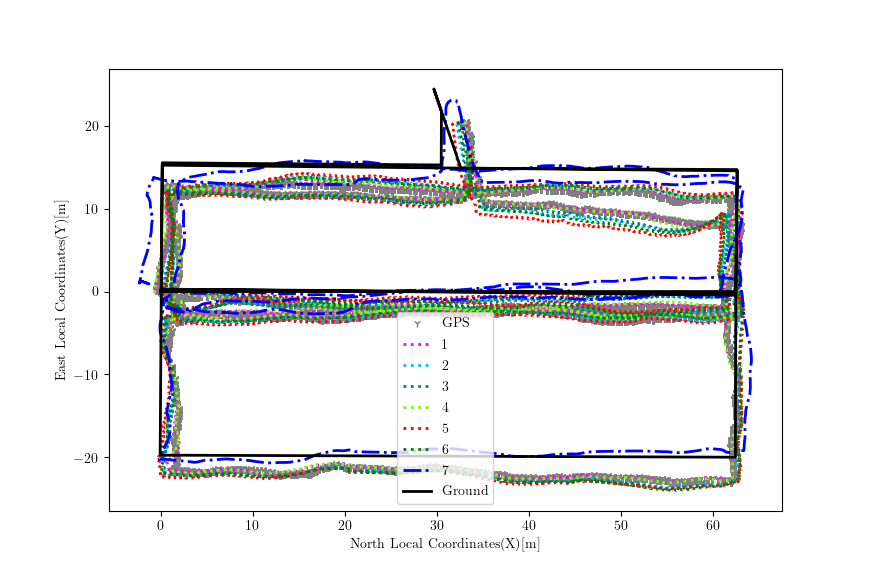
\includegraphics[clip , width=1 \textwidth]{Images/5-Results/GravelLoc.png} % , trim=2cm 1cm 2cm 0.8cm
			\end{center}
			\caption{Comparison of the localisation estimates of six different models on gravel\com{, plus the raw \gls{GPS} position fixes}.\label{fig:gravel-model}}
\end{figure}
%\\~\\

These results of each model, as obtained by averaging the metrics computed at each step, are shown in Table \ref{tab:grav-rmse}.
	\begin{table}[!ht]
		\small
		\begin{center}
			\begin{tabular}{|c|||S[table-format=-1.2]|S[table-format=-1.2]|S[table-format=-1.2]||S[table-format=-1.1(1)]|}
				\hline
				\multirow{3}{*}{\textbf{Model}} & \multicolumn{4}{c|}{\textbf{Evaluation Criteria}} \\
				& \multicolumn{3}{c||}{\textbf{RMSE}} & \multicolumn{1}{c|}{\textbf{Sampling period}}\\
			    & \multicolumn{1}{c|}{$\mathbf{x}$[\SI{}{\meter}]} & \multicolumn{1}{c|}{$\mathbf{y}$[\SI{}{\meter}]} & \multicolumn{1}{c||}{$\boldsymbol \theta$[\SI{}{\radian}]} & \multicolumn{1}{c|}{$\Delta_t \pm \sigma_{\boldsymbol \Delta_t}$ [\SI{}{\milli \second}]} \\
				\hline
				\hline
				\centering{GPS} & 1.33 & 2.88 & 0.76 & 1014 \pm 67 \\
				\hline
				\centering{1} & 1.11 & 2.75  & 0.31 & 11.6 \pm 4.0 \\
				\hline
				\centering{2} & 0.98 & 2.79 & 0.38 & 12.1 \pm 4.1 \\
				\hline
				\centering{3} & 1.03 & 2.77 & 0.35 & 12.0 \pm 4.3 \\
				\hline
				\centering{4} & 1.05 & 2.73 & 0.34 & 11.7 \pm 4.0 \\
				\hline
				\centering{5} & 0.92 & 2.83 & 0.42 & 11.9 \pm 3.9 \\
				\hline
				\centering{6} & 1.00 & 2.77 & 0.36 & 12.0 \pm 4.0 \\
				\hline
				\centering{7} & 0.95 & 1.18 & 0.51 & 10.1 \pm 5.1 \\
				\hline
			\end{tabular}
			\caption{Gravel experiment results.\label{tab:grav-rmse}}
		\end{center}
	\end{table}

The final poses' offsets as obtained by the different models, along with their related estimated standard deviation, are shown in Table \ref{tab:final-gravel}.
	\begin{table}[!ht]
		\small
		\begin{center}
			\begin{tabular}{|c||S[table-format=-1.2(4)]|S[table-format=-1.2(1)]|S[table-format=-1.2(1)]|}
				\hline
				\multirow{2}{*}{\textbf{Model}} & \multicolumn{3}{c|}{\textbf{Final Offset $\pm$ Uncertainty}} \\
				& \multicolumn{1}{c|}{$\mathbf{x} \pm \sigma_\mathbf{x}$[\SI{}{\meter}]} & \multicolumn{1}{c|}{$\mathbf{y} \pm \sigma_\mathbf{y}$[\SI{}{\meter}]} & \multicolumn{1}{c|}{$\boldsymbol \theta  \pm \sigma_{\boldsymbol \theta}$[\SI{}{\radian}]} \\
				\hline
				\hline
				\centering{GPS} & 0.38 \pm 3.25 & 0.50 \pm 3.25 & 0.58 \pm 0.27 \\
				\hline
				\centering{1} & 0.36 \pm 0.58 & 0.60 \pm 1.39 & 0.57 \pm 0.04 \\
				\hline
				\centering{2} & 0.51 \pm 0.62 & 0.68 \pm 0.55 & 0.54 \pm 0.01 \\
				\hline
				\centering{3} & 0.41 \pm 0.47 & 0.72 \pm 0.55 & 0.57 \pm 0.54 \\
				\hline
				\centering{4} & 0.37 \pm 0.20 & 0.65  \pm 0.89 & 0.84 \pm 0.04 \\
				\hline
				\centering{5} & 0.58 \pm 0.37 & 0.72  \pm 0.33 & 0.42 \pm 0.01 \\
				\hline
				\centering{6} & 0.48 \pm 0.29 & 0.66 \pm 0.31 & 0.55 \pm 0.01 \\
				\hline
				\centering{7} & 1.32 \pm 0.41 & 0.38 \pm 0.39 & 0.26 \pm 0.01 \\
				\hline
			\end{tabular}
			\caption{Gravel experiment final results.\label{tab:final-gravel}}
		\end{center}
	\end{table}



\com{
\begin{figure}[!ht]
	\begin{center}
		\begin{subfigure}[b]{.495\textwidth}
			\begin{center}
				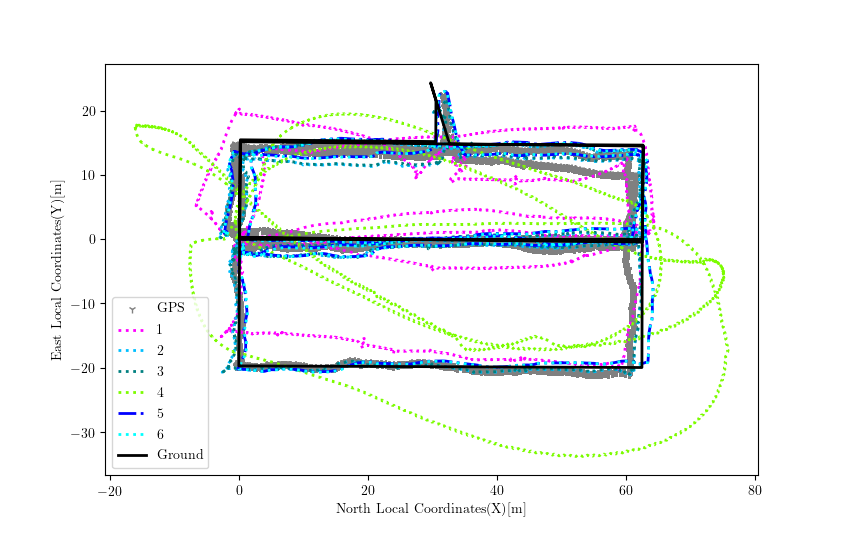
\includegraphics[width=1\textwidth]{Images/5-Results/Gravel-KF.png}
			\end{center}
			\caption{Different filters comparison}
			\label{fig:d435}
		\end{subfigure}
		\begin{subfigure}[b]{.495\textwidth}
			\begin{center}
				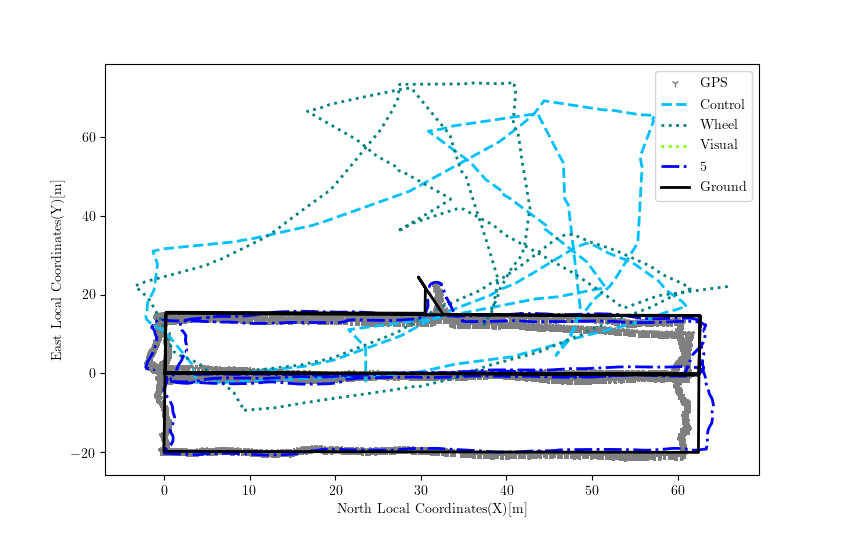
\includegraphics[width=1\textwidth]{Images/5-Results/Gravel-Loc.png}
			\end{center}
			\caption{Best filter performance}
			\label{fig:d435}
		\end{subfigure}%
		\caption{Localisation on gravel results.}
		\label{fig:camera_sensor}
	\end{center}
\end{figure}
}


\subsection{Grass Validation Experiment }
\noindent
This test was run on an even ground with long grass.
This experiment is run using the same techniques, defined in the Method chapter, adopted for the previous experiment.
This has been done to try to validate the calibration and localisation performance provided by the same models on different settings.

The following localisation performance have been obtained by executing the different configurations of sensors and retrieving their localisation evaluations, as before.
%\\~\\
The estimates of all the modules are shown as obtained at each step by them in Figure \ref{fig:grass-models}.
\begin{figure}[!ht]
			\begin{center}
				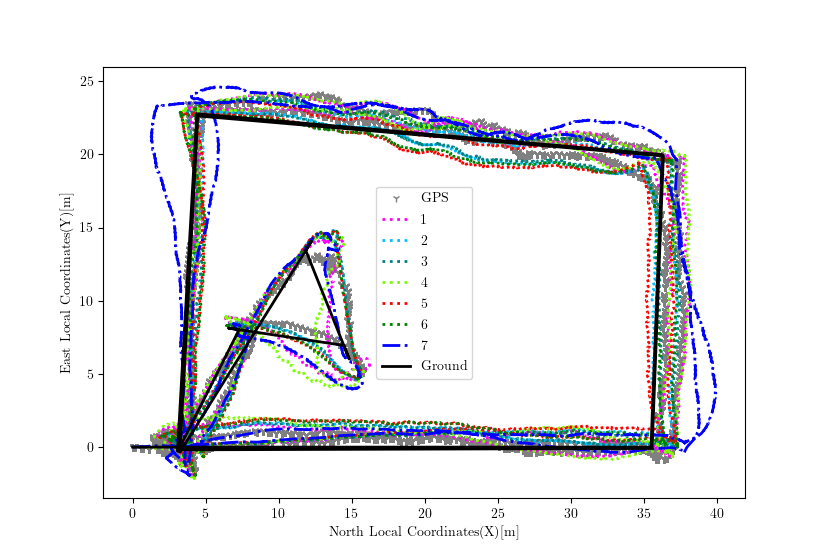
\includegraphics[clip, width=1 \textwidth]{Images/5-Results/GrassLoc.png} %, trim=2cm 1cm 2cm 0.8cm
			\end{center}
			\caption{Comparison of the localisation estimates of different models on grass.}
	\label{fig:grass-models}
\end{figure}

These results of each model, as obtained by averaging the metrics computed at each step, are shown in Table \ref{tab:grass-eval}.
	\begin{table}[!ht]
		\small
		\begin{center}
			\begin{tabular}{|c|||S[table-format=-1.2]|S[table-format=-1.2]|S[table-format=-1.2]||S[table-format=-1.2(1)]|}
				\hline
				\multirow{3}{*}{\textbf{Model}} & \multicolumn{4}{c|}{\textbf{Evaluation Criteria}} \\
				& \multicolumn{3}{c||}{\textbf{RMSE}} & \multicolumn{1}{c|}{\textbf{Sampling period}}\\
			    & \multicolumn{1}{c|}{$\mathbf{x}$[\SI{}{\meter}]} & \multicolumn{1}{c|}{$\mathbf{y}$[\SI{}{\meter}]} & \multicolumn{1}{c||}{$\boldsymbol \theta$[\SI{}{\radian}]} & \multicolumn{1}{c|}{$\Delta_t \pm \sigma_{\boldsymbol \Delta_t}$ [\SI{}{\milli \second}]} \\
				\hline
				\hline
				\centering{GPS} & 1.86 & 1.33 & 0.84 & 1020 \pm 74 \\
				\hline
				\centering{1} & 1.68 & 1.49  & 0.37  & 10.3 \pm 3.5 \\
				\hline
				\centering{2} & 1.58 & 1.44 & 0.26 & 10.8 \pm 3.8 \\
				\hline
				\centering{3} & 1.50 & 1.41 & 0.21 & 10.8 \pm 3.8 \\
				\hline
				\centering{4} & 1.84 & 1.60 & 0.40 & 10.3 \pm 3.5 \\
				\hline
				\centering{5} & 1.81 & 1.55 & 0.30 & 10.9 \pm 3.8 \\
				\hline
				\centering{6} & 1.66 & 1.49 & 0.25 & 10.9 \pm 3.8 \\
				\hline
				\centering{7} & 1.49 & 0.89 & 0.47 & 9.5 \pm 7.0 \\
				\hline
			\end{tabular}
			\caption{Grass experiment results.\label{tab:grass-eval}}
		\end{center}
	\end{table}
%\\~\\~\\~\\~\\

The final poses' offsets as obtained by the different models, along with their related estimated standard deviation, are shown in Table \ref{tab:grass-final}.
	\begin{table}[!ht]
		\small
		\begin{center}
			\begin{tabular}{|c||S[table-format=-1.2(4)]|S[table-format=-1.2(1)]|S[table-format=-1.2(1)]|}
				\hline
				\multirow{2}{*}{\textbf{Model}} & \multicolumn{3}{c|}{\textbf{Final Offset $\pm$ Uncertainty}} \\
				& \multicolumn{1}{c|}{$\mathbf{x} \pm \sigma_\mathbf{x}$[\SI{}{\meter}]} & \multicolumn{1}{c|}{$\mathbf{y} \pm \sigma_\mathbf{y}$[\SI{}{\meter}]} & \multicolumn{1}{c|}{$\boldsymbol \theta  \pm \sigma_{\boldsymbol \theta}$[\SI{}{\radian}]} \\
				\hline
				\hline
				\centering{GPS} & 1.47 \pm 2.50 & 0.14 \pm 2.50 & 0.62 \pm 0.20 \\
				\hline
				\centering{1} & 1.35 \pm 0.35 & 0.20 \pm 1.37 & 0.59 \pm 0.01 \\
				\hline
				\centering{2} & 1.44 \pm 0.19 & 0.23 \pm 0.81 & 0.58 \pm 0.01 \\
				\hline
				\centering{3} & 1.43 \pm 0.18 & 0.24 \pm 0.80 & 0.58 \pm 0.01\\
				\hline
				\centering{4} & 1.31 \pm 0.30 & 0.17 \pm 0.74 & 0.60 \pm 0.02 \\
				\hline
				\centering{5} & 1.36 \pm 0.15 & 0.21 \pm 0.46 & 0.59 \pm 0.01 \\
				\hline
				\centering{6} & 1.36 \pm 0.15 & 0.21 \pm 0.46 & 0.59 \pm 0.01 \\
				\hline
				\centering{7} & 1.34 \pm 0.06 & 0.14 \pm 0.06 & 0.60 \pm 0.02 \\
				\hline
			\end{tabular}
			\caption{Grass experiment final results.
			\label{tab:grass-final}}
		\end{center}
	\end{table}
	

\com{
\begin{figure}[!ht]
	\begin{center}
		\begin{subfigure}[b]{.495\textwidth}
			\begin{center}
				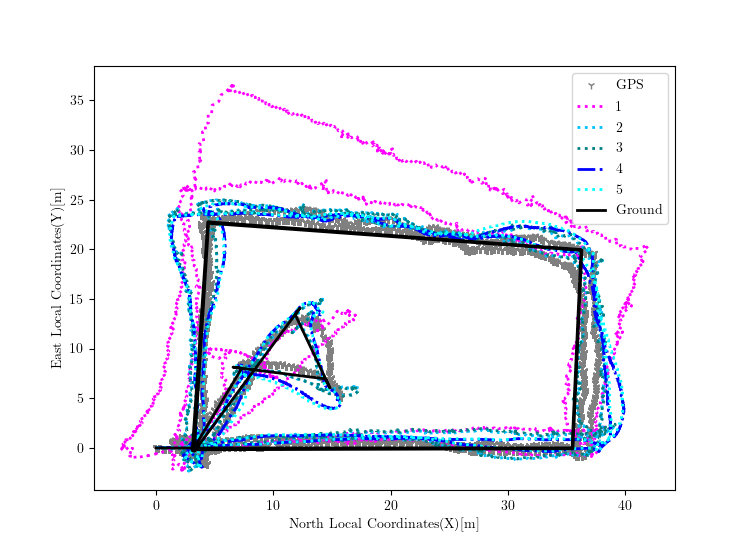
\includegraphics[width=1\textwidth]{Images/5-Results/Grass4-KF.png}
			\end{center}
			\caption{Different filter comparison}
			\label{fig:d435}
		\end{subfigure}
		\begin{subfigure}[b]{.495\textwidth}
			\begin{center}
				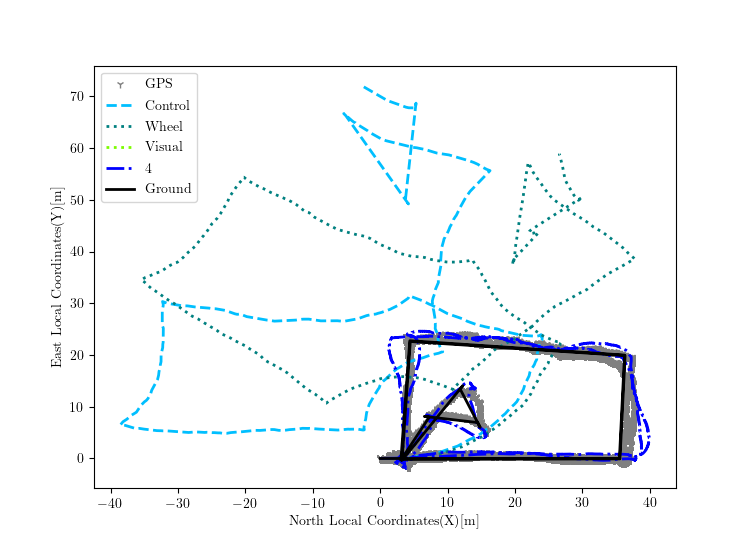
\includegraphics[width=1\textwidth]{Images/5-Results/Grass4-Loc.png}
			\end{center}
			\caption{Best filter performance}
			\label{fig:d435}
		\end{subfigure}%
		\caption{Localisation on grass results }
		\label{fig:camera_sensor}
	\end{center}
\end{figure}
}


\subsection{Discussion on Localisation}
\noindent
Using a sensor fusion approach, such as \gls{EKF}, it is possible to improve the localisation performance of an \gls{ALM}.
The results show how the localisation's configuration improves the estimate of the pose in real-time with respect to the \gls{GPS} receiver raw measurements.
The best positioning module is obtained by not considering control, adopting an orientation model for the \gls{GPS} and adding \glspl{IMU}, which are exploited to improve the angular velocity estimation and to model the process system noise in the prediction step of the \gls{EKF}. % with a configuration which enables for dynamic system noise generation.
The sensor fusion with an adaptive approach manages to provide the best performance using the available sensors.
It exploits the varying noise parameters determining them at each step, which are based on the measurements obtained.
Moreover, the adaptive approach also exploits the initial calibration and the already available dynamic covariance for the sensor to provide the most accurate corrections as possible.

The overall best performance is obtained by "\textit{Model 7}".
However, the results are still not the one initially desired.
Recalling the localisation research questions defined in Section \ref{sec:res-goals}, it is clear that the overall error is around two times bigger than the one defined by the research question.
Moreover, the final offset is around one and half bigger than what was expected by the research question.


As the assumptions are non perfectly validated and non-linearities are present, the performance of the \gls{EKF} are limited to a non perfect estimator. "\textit{Models 1-6}" employ a more correct \gls{EKF} approach and therefore manage to accurately use the measurements available, but this approach provides worse overall performance as the \gls{GPS} measurements are not disturbed by the assumed additive white gaussian noise. 
The receiver has \gls{INS} characteristics, and thus the measurements retrieved and fused while the automower is moving are bringing the \gls{EKF} estimates to converge into the \gls{GPS} measurements.
However, as these measurements are still far from precise and slower to react than the actual ground truth, these correct implementations based on wrong assumptions worsen the localisation performance with respect to the last Model in which the positions' estimates have less influence on the sensor fusion system. 
%, e.g., the noise model of the sensors is not entirely defined by a gaussian white noise model in the case of the \gls{GPS} receiver, so its measures are not fused in properly in the correction step.
Another limitation could be given by the low computational power provided by the embedded device, considering that during the experiments both the recording of the measurements and the mapping module were performed.


\com{
A relevant configuration to be considered is the one given by "\textit{Model 4}".
Given its most basic combination of sensors, it can be shown how that model drifts away.
This result is given by the fact that the \gls{GPS} noise covariance is high, thus its raw measurements alone are not precise enough to correct the estimates in a timely manner.
Moreover, the drifting behaviour is given by the lack of correcting factors, offered by checking the control values or by setting the process noise covariance matrix dinamically with the \glspl{IMU} estimates, to limit the orientation estimate errors, as they are provided by the \gls{GPS} measurement model.}

Finally, the performance of "\textit{Model 7}" are compared with the related measures adopted by the sensor fusion filter, as obtained during both the gravel and grass experiments.
Those results are shown below in Figure \ref{fig:5-gravel} and in Figure \ref{fig:grass-5} respectively.
\begin{figure}[!ht]
			\begin{center}
				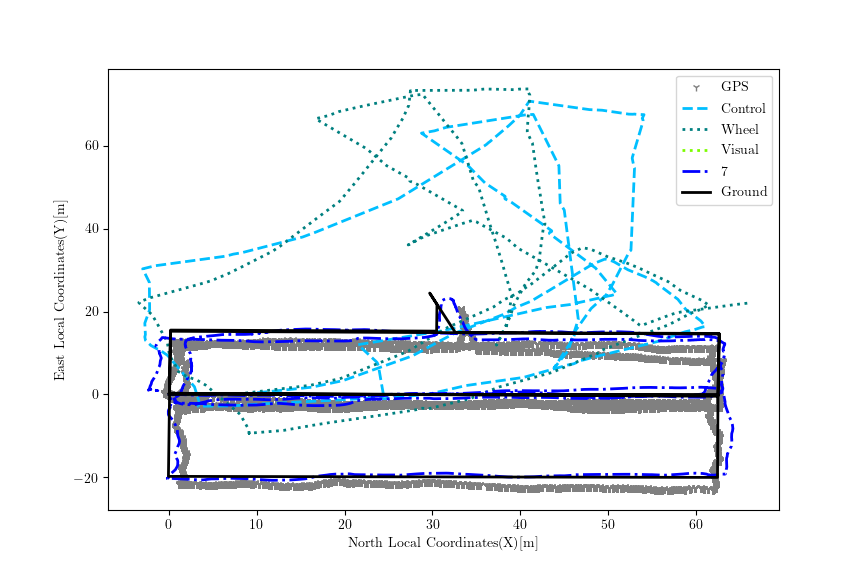
\includegraphics[clip, width=0.78 \textwidth]{Images/5-Results/GravelKF.png} %, trim=2cm 1cm 2cm 0.8cm
			\end{center}
			\caption{Best filter performance on gravel.}
	\label{fig:5-gravel}
\end{figure}
\begin{figure}[!ht]
			\begin{center}
				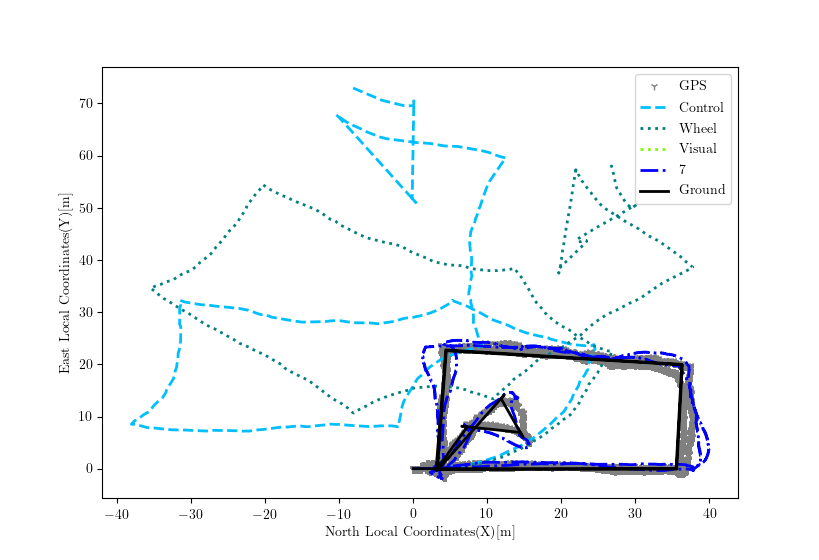
\includegraphics[clip , width=0.78 \textwidth]{Images/5-Results/GrassKF.png} %, trim=2cm 1cm 2cm 0.8cm
			\end{center}
			\caption{Best filter performance on grass.}
	\label{fig:grass-5}
\end{figure}

\com{
\begin{figure}[!ht]
	\begin{center}
		\begin{subfigure}[b]{.495\textwidth}
			\begin{center}
				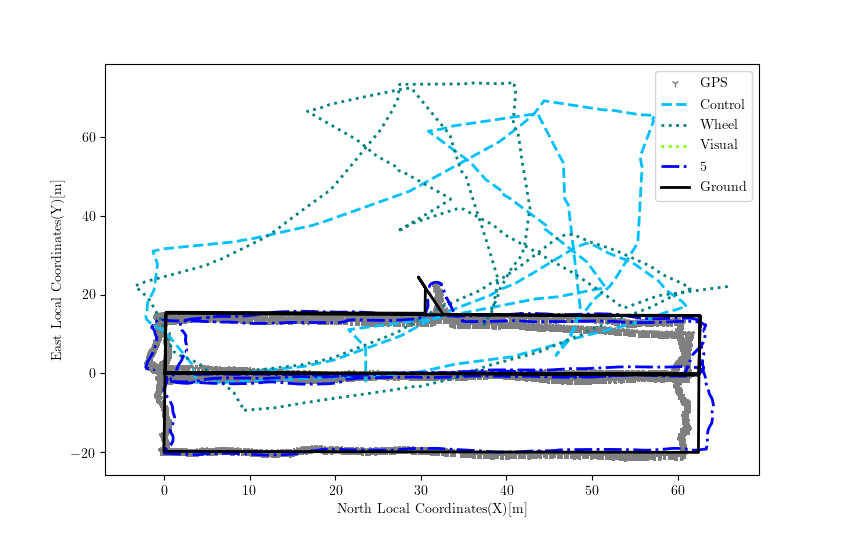
\includegraphics[clip, trim=2cm 1cm 2cm 0.8cm , width=0.8 \textwidth]{Images/5-Results/Gravel-Loc.png}
			\end{center}
			\caption{Best filter performance on gravel.}
	\label{fig:5-gravel}
		\end{subfigure}
		\begin{subfigure}[b]{.495\textwidth}
			\begin{center}
				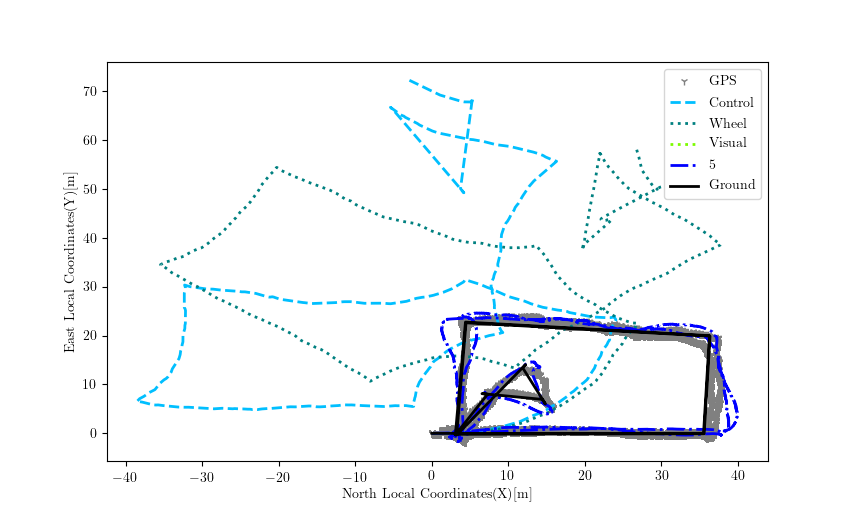
\includegraphics[clip, trim=2cm 1cm 2cm 0.8cm , width=1 \textwidth]{Images/5-Results/Grass-Loc.png}
			\end{center}
			\caption{Best filter performance on grass.}
	\label{fig:grass-5}
		\end{subfigure}%
		\caption{Localisation on grass results }
		\label{fig:camera_sensor}
	\end{center}
\end{figure}
}


\section{Mapping Analysis}
\noindent The evolution of the mapping feature is shown, from the initial setting of the occupancy grid, to the customised virtual boundary generation, and finally to the updating map behaviour.

The configuration model chosen to localise the \gls{ALM} for this module is "\textit{Model 7}", as defined in Section \ref{sec:locRes}. 
The mapping method is highly reliant on precise estimation, and the real-time requirement is especially important in case of collision events, to make sure that they are mapped to their related and timely position.

The experiments used to evaluate the mapping module are the same used for the localisation analysis, i.e., the gravel and grass experiments.
Those have been chosen for their length and completeness.
The initial test on the gravel simply defines the boundaries of the environment, defining two different zones, which could be handled differently.
On the grass test, after the virtual boundary generation, the map is also updated using eventual collision's events to account for objects present on the lawn.

The results from the map generated from the estimates provided by the localisation module are compared with a map computed with the same technique but using the ground truth trajectory.
With this approach, it is possible to check if the estimated map matches the real outdoor environment.

Their evaluation will be split between the Complete map, the Boundary definition, and the Collision identification.
On the Complete section, all the cells of the occupancy grids will be used to generate the results.
The Boundary evaluation will be computed using the cells set to the negative value $-1$, as specified, by either the ground truth or the estimate.
A similar approach will be adopted for the Collisions, using a threshold of value $25$ to distinguish between occupied and not-occupied cells.
For each category, all of the evaluation metrics defined in the methods will be performed wherever possible.

\subsection{Gravel Boundary Experiment}
\noindent
As defined before, the gravel experiment is performed to build the virtual boundary specifying two different areas.
The \gls{ALM} simply updates the cells related to its estimated pose with the negative value defined. 


The overlapped maps obtained by such a boundary definition, using both the ground truth and the \gls{EKF} estimates, are shown below in Figure \ref{fig:occGridBoud}. 
\begin{figure}[!ht]
	\begin{center}
		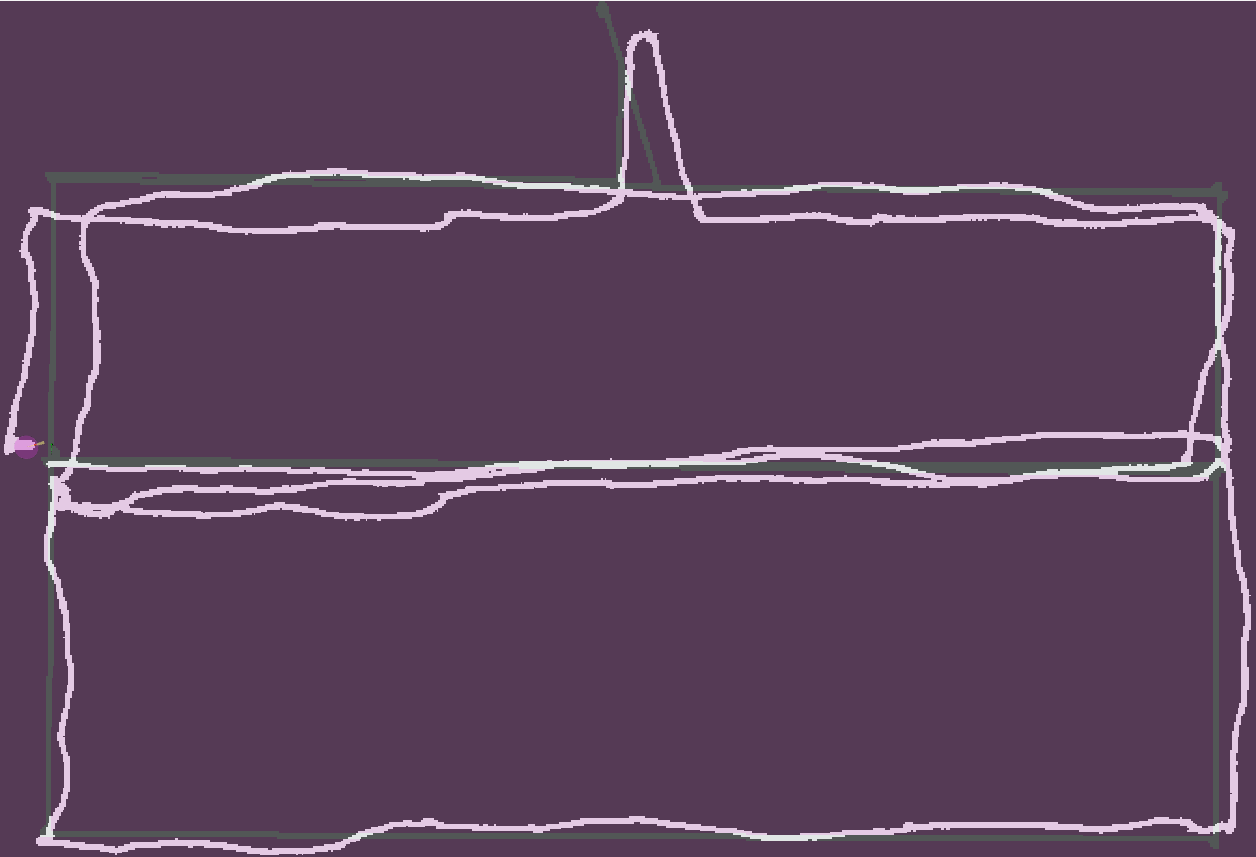
\includegraphics[width=0.7\textwidth]{Images/5-Results/Gravel5.png}
	\end{center}
	\caption{Personalised boundary definition for overlapped maps\\defined by ground truth(grey) and estimated(white).\centering}
	\label{fig:occGridBoud}
\end{figure}
%\\~\\

The results obtained by comparing the ground truth map with the estimated results are shown in Table \ref{tab:map-gravel}.\begin{table}[!ht]
	\small
	\begin{center}
		\begin{tabular}{|c||S[table-format=-1.2]|}
			\hline
			\centering{\textbf{Section}} & \multicolumn{1}{c|}{\centering{\textbf{Map Score}}}\\
			\hline
			\hline
			\centering{Complete} & 12.9    \\
			\hline
			\centering{Boundary} & 46.4  \\
			\hline
		\end{tabular}
		\caption{Gravel Mapping Results\label{tab:map-gravel}}
	\end{center}
\end{table}
\com{
\begin{table}[!ht]
	\small
	\begin{center}
		\begin{tabular}{|c||S[table-format=-1.2]|S[table-format=-0.2]|S[table-format=-0.2]|}
			\hline
			\multirow{2}{*}{\textbf{Section}} & \multicolumn{3}{c|}{\textbf{Evaluation Metric}}\\
			& \multicolumn{1}{c|}{$MS$} & \multicolumn{1}{c|}{$PCC$} & \multicolumn{1}{c|}{$F1$} \\
			\hline
			\hline
			\centering{Complete} & 12.9 & 0.27 &   \\
			\hline
			\centering{Boundary} & 46.4 & -0.69 & 0.30  \\
			\hline
		\end{tabular}
		\caption{Gravel Mapping Results\label{tab:map-gravel}}
	\end{center}
\end{table}
}

\subsection{Grass Final Experiment}
\noindent
The grass experiment evaluates the performance of the complete and final system.
It starts by building the virtual boundary running the same perimeter two times.
Afterwards, it runs inside the defined area to test the dynamic map update exploiting the collisions' sensors.
In this specific case, 3 different collision events are fired, then the \gls{ALM} is made to rotate and continue until its next collision.
At the third collision event, the mobile robot is commanded to return to its origin.


The overlapped maps obtained by such definitions using both the ground truth and the \gls{EKF} estimates are shown below in Figure \ref{fig:occGridBoud} and the related evaluation results obtained by comparing the ground truth map with the estimated results are shown in Table  \ref{tab:map-grass}.

\begin{figure}[!ht]
	\begin{center}
		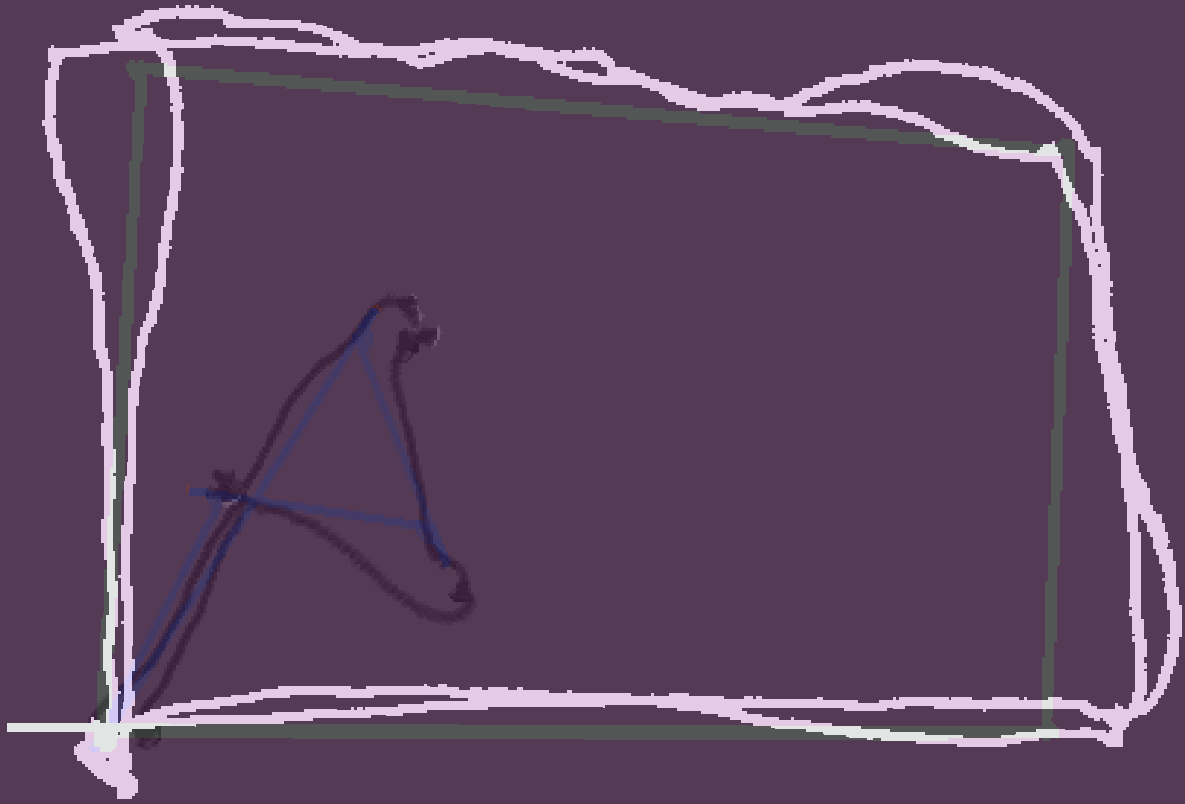
\includegraphics[width=0.75\textwidth]{Images/5-Results/Grass5.png}
	\end{center}
	\caption{Update of the map inside the boundaries (lighter shade means probability of object given by collision events)}
	\label{fig:occGridUpdate}
\end{figure}

\begin{table}[!ht]
	\small
	\begin{center}
		\begin{tabular}{|c||S[table-format=-1.2]|}
			\hline
			\centering{\textbf{Section}} & \multicolumn{1}{c|}{\centering{\textbf{Map Score}}}\\
			\hline
			\hline
			\centering{Complete} & 9.51    \\
			\hline
			\centering{Boundary} & 44.9  \\
			\hline
			\centering{Collisions} & 45.4  \\
			\hline
		\end{tabular}
		\caption{Grass Mapping Results
		\label{tab:map-grass}}
	\end{center}
\end{table}
\com{
\begin{table}[!ht]
	\small
	\begin{center}
		\begin{tabular}{|c||S[table-format=-1.2]|S[table-format=-0.2]|S[table-format=-0.2]|}
			\hline
			\multirow{2}{*}{\textbf{Section}} & \multicolumn{3}{c|}{\textbf{Evaluation Metric}}\\
			& \multicolumn{1}{c|}{$MS$} & \multicolumn{1}{c|}{$PCC$} & \multicolumn{1}{c|}{$F1$} \\
			\hline
			\hline
			\centering{Complete} & 9.51 & 0.34 &   \\
			\hline
			\centering{Boundary} & 44.9 & -0.62 & 0.35  \\
			\hline
			\centering{Collisions} & 45.4 & -0.84 & 0.07  \\
			\hline
		\end{tabular}
		\caption{Grass Mapping Results
		\label{tab:map-grass}}
	\end{center}
\end{table}
}

\subsection{Discussion on Mapping}
\noindent
The overall mapping results showcase how the generation of a reliable and accurate perception of the environment is still not possible.
This is given by the dependence on the localisation's performance, which are still not good enough to then exploit them for this purpose.

Related to the mapping module performance on its own, however, it is noticeable how effective the proposed approach could be.
The ground truth map, as obtained by using the ground truth trajectory to define both boundaries and collision events, exploits the same functionalities defined for the \gls{EKF} estimates and provides the features needed.


\cleardoublepage
%\clearpage


    \chapter{Conclusions}
\label{ch:conclusion}

DRAFT

\noindent
This project managed to fuse the measurements of multiple and heterogeneous sensors.
It has been demonstrated how the implementation of this sensor fusion technique exploited a subset of sensors to achieve more accurate localisation estimates.
Moreover, the mapping feature has been achieved by setting virtual boudaries through initial runs and then updating its knowledge using collision sensor events.

\section{Discussions}
\label{sec:discussion}
\com{
\todo[inline]{Describe the conclusions (reflect on the whole introduction given in Chapter 1).}

	Discuss the positive effects and the drawbacks.\\
	Describe the evaluation of the results of the degree project.\\
	Did you meet your goals?\\
	What insights have you gained?\\
	What suggestions can you give to others working in this area?\\
	If you had it to do again, what would you have done differently?\\
}


\noindent After this master thesis, two related topics have been investigated.
The findings are discussed below.


\subsection{Localisation}
\noindent
Using a sensor fusion approach, such as \gls{AEKF}, it is possible to reach fast and robust localisation estimates.

Not all the sensors behaved as expected and the best configuration has not been achieved using all the sensors available as expected.

\subsection{Mapping}
\noindent
With the improved localisation, it is possible to limit the mowing area of the \gls{ALM} using a virtual boundary.

Using collision sensors and accounting for the robot pose uncertainty it is possible to provide a better understanding of the robot environment.


\section{Limitations}
\label{sec:limitations}
\com{
\todo[inline]{What did you find that limited your
  efforts? What are the limitations of your results?}
}
\noindent As the system has been tested experimentally on the field, the conditions to run it outside were needed.
This limited the available amount of time to do outdoor testing in a relevant matter, especially given the raining days.

Being the system an hardware implementation, different aspects needed to be tested before running the tests, removing time to more advanced tuning of the implementation.

\section{Future works}
\label{sec:futureWork}
\com{
\todo[inline]{Describe valid future work that you or someone else could or should do.\\
Consider: What you have left undone? What are the next obvious things to be done? What hints can you give to the next person who is going to follow up on your work?
}
}
\com{
Due to the breadth of the problem, only some of the initial goals have been
met. In these section we will focus on some of the remaining issues that
should be addressed in future work. ...
}

\com{
In particular, the author of this thesis wishes to point out xxxxxx remains as
a problem to be solved. Solving this problem is the next thing that should be
done. ...
}

\noindent
Expanding the states of the system in order to navigate in a 3D environment instead than a simple 2D environment as in this project.
It will be possible to account for slopes in the lawn and it could be interesting to evaluate its influence in the GPS readings.


It could be investigated a trade off between computations needed for a reliable SLAM implementation instead of an online implementation provided in this report.


Exploit depth information from the camera to provide a faster identification of collision events, eventually providing a map of the environment based on depth information instead of collision events.
Instead of using the collision sensors to update the map, the camera, and its depth readings,  could be used for object detection to identify and avoid the objects before collision.


Outliers detection in case of non reliable sensors and once the covariances noises matrices have been ultimately perfected. Moreover, it can be crucial when the sensors are not behaving correctly.


Intrinsic and Extrinsic Calibration\\
Currently, we are considering the case of a mobile
robot whose odometry is not calibrated. In this case,
the observability analysis will extend to the parameters
characterizing the odometry error (e.g. wheel diameters,
distance between the wheel).


Path planning algorithm as in~\cite{coveragePathplanning} and \cite{machines6040046}, can be used to provide coverage features to the autonomous lawn mowers.
A comprehensive overview about coverage is available in \cite{galceran_survey_2013}. It discusses all the available techniques and their related strengths and weaknesses.
More specific approaches to be investigated can be found in \cite{hameed_coverage_2017} and \cite{cabreira_grid-based_2019}.
Regarding the avoidance of the objects for the unexpected detection of objects, a techniques is define in \cite{daltorio_obstacle-edging_2010}.



\section{Reflections}
\com{
\todo[inline]{What are the relevant economic, social,
  environmental, and ethical aspects of your work?
  }
}
\label{sec:reflections}

\noindent This project will address the following ethics and sustainability issues:
\begin{itemize}
    \item Waste reduction: keeping the localisation module included in the automower will remove the need to install additional infrastructure which could then be susceptible to deterioration.
    \item Bees preservation: Thanks to a more accurate control of the lawn with a given map, it will be possible to dynamically update it and preserve a part of the lawn to allow bees to prosper, without intervening on the boundary wire.
    \item Privacy issue: the images needed for the visual odometry module are going to be used inside the automower, not shared outside of it. They will be destroyed after their processing, avoiding breach of personal privacy in case of theft of the memory card.
    \item Economic aspects: as the \gls{ALM} is a consumer product, the comparison between the available and proposed approach is relevant. A cheaper solution that provides more features might attract more customers.
\end{itemize}

\subsection{Environmental}
\noindent
With a more precise localisation and navigation system the intervention on the lawn will be reduced.
Also, the external boundary configuration produces some wastes that the virtual boundary do not have.

Moreover, with the possibility to set virtual boundaries for the automower, it will be possible to save part of the lawn for bees to find flowers to sustain themselves and prosper.


\subsection{Security}
\noindent

The system is self-contained, and every information is stored inside the embedded Raspberry Pi 4.
The single output that might be relevant to share can be the current position of the automower and the updated map that he has available for navigation.

The online system that doesn't store the history of the states also helps with the security of the information stored.

It can be easily protected through a password to avoid theft of information.
The SD card could be encrypted also to avoid theft of it and retrieval of information through that memory.

\subsection{Economical Analysis}
\com{
The current prototype works, but the performance from a cost perspective makes
this an impractical solution. Future work must reduce the cost of this
solution, to do so a cost analysis needs to first be done. ...
}
\noindent
As an economic results, by simply adding additional GPS, IMU, and RGB-D camera it is possible to remove the need of the boundary wire.
As such, by adding to the automower the cost of these additional sensors it will be possible to save money in the additional maintenance required.
Overall, given the high reliability over time of these sensor, the consumers will be able to save money in the long run.
However, the product-market fit might not be the best, since the company that will sell the automower also provides the boundary wire and removing that need will economically lower their revenues in that aspects. Anyway, the customers will be more willing to buy a system that requires less maintenance.
So the trade-off will be between the more services offered and the lower revenues from selling additional infrastructures.
Analysis of costs of sensors and usual boundary wire, plus related maintenance

It saves also the energy that now is given to the boundary wire to power the magnetic field that the automower need to detect its boundaries now.

\com{
The thesis contributes to the \gls{UN}\enspace\glspl{SDG} numbers 1 and 9 by
xxxx.
}


\cleardoublepage
%\clearpage


    
% Print the bibliography (and make it appear in the table of contents)
%\printbibliography[heading=bibintoc]
% The lines below are for BibTeX
\bibliographystyle{Input/myIEEEtran}
\renewcommand{\bibname}{References}
\addcontentsline{toc}{chapter}{References}
\bibliography{Input/Chapters/8-References}

%\noindent\rule{\textwidth}{0.4mm}
\com{
\todo[inline]{In the references, let Zotero or other tool fill this
  in for you. I suggest an extended version of the IEEE  style, to include
  URLs, DOIs, ISBNs, etc., to make it easier for your reader to find
  them. This will make life easier for your opponents and examiner. \\

  IEEE Editorial Style Manual: \url{https://www.ieee.org/content/dam/ieee-org/ieee/web/org/conferences/style_references_manual.pdf}
}
}
\cleardoublepage
%\clearpage


    
\appendix
\renewcommand{\chaptermark}[1]{\markboth{Appendix \thechapter\relax:\thinspace\relax#1}{}}
\com{
\chapter{Model of the sensors}


\section{Kinematic Model}
\noindent
$$
  \label{eq:state}
\mathbf{X}_t=
\begin{bmatrix}
\mathbf{x}_t \\ \mathbf{y}_t \\ \boldsymbol \theta_t \\ \mathbf{v}_t \\ \boldsymbol \omega_t \\ \mathbf{a}_t \\[0.3em]
\end{bmatrix}
$$

\begin{equation}
A_t
=
\begin{bmatrix}
1 & 0 & 0 & dt \cdot \cos(\boldsymbol \theta_t) & 0 & \frac{dt^2 \cdot \cos(\boldsymbol \theta_t)}{2} \\
0 & 1 & 0 & dt \cdot \sin(\boldsymbol \theta_t)& 0 & \frac{dt^2 \cdot \sin(\boldsymbol \theta_t)}{2} \\
0 & 0 & 1 & 0 & dt & 0 \\
0 & 0 & 0 & 1 & 0 & dt \\
0 & 0 & 0 & 0 & 1 & 0 \\
0 & 0 & 0 & 0 & 0 & 1 \\[0.3em]
\end{bmatrix}
\end{equation}

\begin{equation}
    \mathbf{X}_t = A \cdot \mathbf{X}_{t-1}
\end{equation}

\section{Wheel Encoder information}

$$
Wheel~meter~per~tick = \frac{( 2 \cdot \pi ) \cdot ( \frac{Wheel~diameter}{2}) }{Wheel~Pulses~per~turn}
$$


$$
\Delta _{PulsesRight} = Right~Pulses - Previous~Right~Pulses
$$
$$
\Delta _{PulsesLeft}  = Left~Pulses  - Previous~Left~Pulses
$$


$$
\Delta _{Right} ~ = \Delta _{PulsesRight} \cdot Wheel~meter~per~tick
$$
$$
\Delta _{Left} ~ = \Delta _{PulsesLeft} \cdot Wheel~meter~per~tick
$$

$$
\Delta s = \frac{\Delta _{Right} + \Delta _{Left}}{2}
$$


$$
\Delta {\theta} = \frac{\Delta _{Right} - \Delta _{Left}}{Base~Width}
$$

\subsection{Euler Encoder Model}

\noindent This is the integration method adopted. It is a precise enough approximation of the
$$
x_{t+1} = x_t + \Delta s \cdot \cos(\theta_t)
$$
$$
y_{t+1} = y_t + \Delta s \cdot \sin(\theta_t)
$$
$$
\theta_{t+1} = \theta_t + \Delta {\theta}
$$

\subsection{Runge-Kutta 2 Encoder Model}

\noindent It is supposed to be slightly more precise, but since the improvements at such an high frequency are non relevant then it is not considered.
$$
x_{t+1} = x_t + \Delta s \cdot \cos(\theta_t + \frac{\Delta{\theta}}{2} )
$$
$$
y_{t+1} = y_t + \Delta s \cdot \sin(\theta_t + \frac{\Delta{\theta}}{2} )
$$
$$
\theta_{t+1} = \theta_t + \Delta {\theta}
$$





\section{GPS}
\noindent
From geodetic coordinates to ENU coordinates, as specified by ROS REP 103 and 105.

Using \com{the tool pymap3d\footnote{https://github.com/geospace-code/pymap3d} or} specific math equations derived by Vincenty solutions of geodesics on the ellipsoid\footnote{Vincenty's formulae  -  Direct and Inverse solutions of geodesics on the ellipsoid with application of nested equations}, through the function geodetic2enu that computest the difference between the initial gps average position of the base station and the current reading obtained by the GPS receiver.

First a translation from the geodetic coordinates in WSG-84 degrees estimated by the GPS receiver sensors to the ECEF coordinates is implemented, it is done so both for the initial coordinate and then used to check the difference with the ECEF translation from the geodetic coordinates of the successive reading of the GPS receiver.


%GPS positioning is in the global coordinate system WGS84 [18].

From World Geodetic System: WGS 84 values
\begin{align}
    EqR &= 6378137 && \text{Equatorial radius (m)} \\
    PoR &= 6356752.3142 && \text{Polar radius (m)}
\end{align}

From which the following can be derived the following values necessary for the next algorithms:
\begin{align}
    f &= \frac{EqR - PoR}{EqR} \\
    e\_sq &= f \cdot (2-f)
\end{align}

Using these values it is possible to transform from Geodetic WSG-84 Coordinates to ECEF coordinates using the  Algorithm specified in \ref{alg:ecef}.


\begin{algorithm}[H]
\caption{Geodetic to ECEF Coordinates }
\label{alg:ecefApp}
  \hspace*{\algorithmicindent} \textbf{Input:} Latitude and Longitude ($lat$, $lon$) in WSG-84 degrees\\
  \hspace*{4em} Altitude ($h$) in meters\\
  \hspace*{\algorithmicindent} \textbf{Output:} ECEF Coordinates in meters ($x$, $y$, $z$)
  %\KwData{Testing set $x$}
  %$\sum_{i=1}^{\infty} := 0$ \tcp*{this is a comment}
  %\tcc{Transform latitude and longitude}
  \begin{algorithmic}[1]
  \STATE $N = \cfrac{EqR}{\sqrt{1 - e\_sq \cdot \sin(lat)^2}}$
  \STATE $x = (h + N) \cdot \sin(lat) \cdot \cos(lon)$
  \STATE $y = (h + N) \cdot \cos(lat) \cdot \sin(lon)$
  \STATE $z = (h + (1 - e\_sq) \cdot N) \cdot \sin(lat)$
  \STATE return $x$, $y$, $z$
    \end{algorithmic}
\end{algorithm}

Finally, by exploiting the previous algorithm, it is possible to transform the Current Geodetic Coordinates into Local Coordinates by using some Reference Geodetic Coordinates and the following Algorithm \ref{alg:local}.

\begin{algorithm}[H]
\caption{Geodetic to Local using Current and Reference Coordinates}
\label{alg:localApp}
    \hspace*{\algorithmicindent} \textbf{Input:} Current Latitude and Longitude ($latC$, $lonC$)\\
        \hspace*{5em} in WSG-84 degrees\\
    \hspace*{4em} Current Altitude ($hC$) in meters\\
    \hspace*{4em} Reference Latitude and Longitude ($latR$, $lonR$)\\
        \hspace*{5em} in WSG-84 degrees\\
    \hspace*{4em} Reference Altitude ($hR$) in meters \\
    \hspace*{\algorithmicindent} \textbf{Output:} Local Coordinates in meters ($\Delta x$, $\Delta y$, $\Delta z$)
  \begin{algorithmic}[1]
    \STATE $xC$, $yC$, $zC$ = Geodetic to ECEF Coordinates ($latC$, $lonC$, $hC$)
    \STATE $xR$, $yR$, $zR$ = Geodetic to ECEF Coordinates ($latR$, $lonR$, $hR$)
    \STATE $xD = xC - xR$
    \STATE $yD = yC - yR$
    \STATE $zD = zC - zR$
    \STATE $\Delta x = -~\sin(lonR)~\cdot~xD~+~\cos(latR)~\cdot~yD$
    \STATE $\Delta y = -~cos(lonR)~\cdot~\sin(latR)~\cdot~xD~-~\sin(latR)~\cdot~\sin(lonR)~\cdot~yD~+ \hspace*{3em} \cos(latR)~\cdot~zD$
    \STATE $\Delta z = \cos(latR)~\cdot~\cos(lonR)~\cdot~xD~+~\cos(latR)~\cdot~\sin(lonR)~\cdot~yD~+  \hspace*{3em} \sin(latR)~\cdot~zD$
    \STATE return $\Delta x$, $\Delta y$, $\Delta z$
    \end{algorithmic}

\end{algorithm}

\com{
\begin{figure}
	\begin{center}
		%\includegraphics{Images/4-Methods/Figure_2.png.eps}
		%\includesvg{Images/4-Methods/Figure_2.png.svg}
		%\input{Images/4-Methods/Original-Fig-GPSfix.pgf}
	\end{center}
	\caption{A PGF histogram from \texttt{matplotlib}.}
\end{figure}
}

\section{IMU}

\noindent
As IMU sensor we use the PhidgetSpatial Precision 3/3/3 High Resolution \footnote{https://www.phidgets.com/?tier=3\&catid=10\&pcid=8\&prodid=1158}.
We use its APIs to gather the measurements and then publish them as ROS topics, after some tunings.

\section{Camera}

\noindent The camera is the Intel RealSense D435 and the \gls{VO} package is \gls{RTABMAP}.

}



\chapter{Competitor Analysis}

\noindent As this master thesis has been developed under the programme of EIT Digital\footnote{\url{https://masterschool.eitdigital.eu/}}, an analysis of the competitor will be performed to highlight the current state of the art at an industrial level for \glspl{ALM} which require no boundary wire installation, understanding their current implementations, and evaluating possible improvements.

Toadi\footnote{\url{https://www.toadi.com/}} is a startup company based in Belgium which offers as only product an \gls{ALM} of the same name. It employs a single visual sensor system to provide the localisation features. It can mow an area of \SI{4800}{\meter\squared}.
Its installation is performed though a track and follow approach to determine the boundaries of the lawn, it has been in testing phase and it is available to the public from May 2021.

The LUNA platform from Inertial Systems\footnote{\url{https://inertialsense.com/autonomy/}} employs all the sensors listed above to provide a localisation and navigation module, which has been used for \glspl{ALM}. This platform was developed to enable engineers to directly embed autonomous capability into existing equipment avoiding the development of a localisation module, as it is detailed in this thesis.

Kingdom Technologies\footnote{\url{https://www.kingdom.garden/}} provide an \gls{ALM} at a monthly fee to commercial clients.
It employs sensor fusion techniques to merge several different sensors' measures to improve the positioning of the robot on a lawn that could reach an area of \SI{7500}{\meter\squared}.

Ambrogio L60 Elite S+\footnote{\url{https://www.ambrogiorobot.com/en/models/view/l60-elite-s}} requires no installation for areas up to \SI{400}{\meter\squared}.
It employs a grass sensor to detect the presence of grass under itself and it uses a specific robotic joint to recognise any holes or empty spaces. With these sensors it is able to navigate around a defined lawn using a reactive approach, but without the need for the boundary wire.

Different approaches which do not require the boundary wire installation but which still need some external infrastructures are the following.

Husvarna 550 EPOS\footnote{\url{https://www.husqvarna.com/us/products/robotic-lawn-mowers/models/automower-550-epos/}} is a new \gls{ALM} available for commercial customers which employs a \gls{GPSRTK} sensor to cover areas of \SI{5000}{\meter\squared}. It needs an external and expensive receiver to correct the \gls{GNSS} estimates of the robot and improve its localisation performance to just a few centimeters error.

iRobot Terra t7\footnote{\url{https://www.irobot.co.uk/Terra}} is the \gls{ALM}
It relies on wireless navigation beacons installed on the garden to triangulate the position of the mower using their signals. However, the implementation of such technology has concerned the \gls{NRAO}, as the original intended frequency they used were disturbing the measurements of that organisation, and they had to change their beacons using \gls{UWB} signal technology.

The currently developed \glspl{ALM} are still far from being mature and available to all customers.
For this reason, an analysis of the best configuration of sensors to improve on the localisation aspects without the need for an external installation is provided, as improved localisation performance of autonomous mobile robots are required.

Numerous related studies and implementations have been developed in similar topics to improve localisation features, and the analysis of an optimal configuration of sensors which require no external installations is still relevant to the best of the found knowledge.



\chapter{Highly-Non-Linear Sensor Fusion}
\noindent The system analysed in this thesis is not characterised by high non-linearity given the high frame-rate available, and as such the adopted \gls{AEKF} is robust, fast, and sufficient.

A brief description of other linearisations, such as the \gls{UKF}, and other approaches, such as \gls{PF}, are provided in this appendix.
Even if they are not used in this thesis, they are noteworthy to mention to provide a more comprehensive overview of sensor fusion techniques, in case of highly non linear systems.

\section{Unscented Kalman Filter}
\label{sec:ukf}
\noindent The \gls{UKF} is an alternative to the \gls{KF} for estimation of highly non linear systems~\cite{unscentedK}.
Instead of using a linearisation approach, the \gls{UKF} is based on a deterministic sampling method.
The estimates are propagated through the non linear system using sample values, called sigma points, defined by the unscented transform.
This procedure provides two values along the mean of the estimate and symmetrically placed on its main uncertainty axes.
Although the results are not a Gaussian random variables, their mean and standard deviation can be derived from them to maintain the \gls{KF} assumption.

Its improvements in estimates and covariance accuracy are relevant over the \gls{EKF} when the functions $f$ and $h$ are highly non-linear, as it is accurate to the second order Taylor's expansion.
Moreover, it does not need to compute Jacobians of the non linear functions of the system~\cite{thrun_probabilistic_2005}.



\section{Particle Filter}
\label{sec:pf}
\noindent The \gls{PF} provides another implementation of a Bayesian filter~\cite{particle}.
It is an iterative algorithm which saves multiple potential state estimate values, known as particles.
The probability the state estimate value in a moment in time is given by the density of particles nearby which contains similar values.
At each iteration, a sampling phase is performed generating temporary particles using the current estimated state.
Afterwards an importance factor is calculated using new measurements of the state and it provides a likelihood value for the next estimations.
In the resampling phase, the proper particles are updated by using the estimates provided by one of the temporary particles with a selection based on the importance factor.
This process is continuously iterate and the particles will eventually converge to a proper estimate over several steps.

The Rao-Blackwellized \gls{PF} extends it using both particles and Gaussian random variables as state variables~\cite{murphy_rao-blackwellised_2001}.




\chapter{Robotic Operating System}
\label{ch:ros}
\noindent \Gls{ROS}\cite{288} is an open-source framework, and not an actual operating system, widely adopted for building software used to control robotic systems.
\Gls{ROS} works both with C++ and Python programmed scripts, allowing for developers with different backgrounds to develop upon it.


For these nodes to cooperate, they are connected by a middle-layer structure based on a network of topics or services, following a blackboard architecture of data sharing.
It provides a graph-like structure were each program, described as node, can both publish and subscribe messages among the created and available topics.

Topics can be seen as variables which are used for streaming communication and share information between nodes.
A \Gls{ROS} node publishes a specific message through a topic and every other node can subscribe to that topic and receive all the messages posted to it.
A \Gls{ROS} system, to behave as expected, needs a master process which has the task of matching publishers and subscribers to their related topics.

These topics can be generated by sensors, actuators, planners, controllers of different kind and made available using this structure of topics, similar to a blackboard architecture.
Each topic is defined by a specific message type which specifies its content in order to standardise its usage among applications and to simplify communication between nodes.
Messages definition can be customised and they are stored inside the \Gls{ROS} package, defining the data sent within the topic which will use that definition.

Figure \ref{fig:ros-topic} shows an example of a \Gls{ROS} graph where two subscriber nodes receive the messages posted on the topic by a publisher node.

\begin{figure}[!ht]
	%\textbf{Investigating Simultaneous Localization and Mapping for AGV systems}
	\begin{center}
		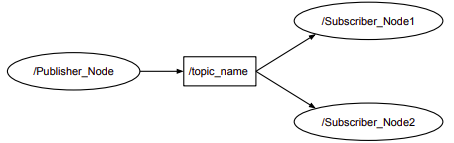
\includegraphics[width=0.75\textwidth]{Images/2-Background/ROSTopic-2021-04-22 10-51-37.png}
	\end{center}
	\caption{\Gls{ROS} topics architecture}% for information sharing\cite{palsson_investigating_2017}}
	\label{fig:ros-topic}
\end{figure}

The aspect of localisation is important for the robotics field, to understand where the robot is located with respect to the rest of the world, but also to know how the sensors are positioned with respect to the robot in which they are installed.
It is of prominent importance to be aware of the different pose of the connected sensors before fusing their information, as the measurements of each sensors are related to their specific coordinate frame.

Before performing sensors fusion, every different frames of the sensors need to be transformed into the base frame of the robot which they are measuring to be sure about that the measurements refers to the same coordinate frame.

\Gls{ROS} uses the TF\cite{6556373} library to provide the tools needed to work with coordinate frames and to deal with their related transformation.
It allows for the definition of each sensor rigid body transform to specify their related position with respect to the robot, and then the library will deal with all the other transformations by publishing messages regarding to the rotational and translational relations between frames.
Commonly used frames are odom and base\_link. The odom frame has the origin at the initial position $P_{odom}$ of the robot and it is used to keep track of its moving behaviour. The base\_link frame is rigidly attached to the robot base $P_{base}$ and it is used to define the frames of its attached components.

\begin{figure}[!ht]
	%\textbf{Investigating Simultaneous Localization and Mapping for AGV systems}
	\begin{center}
		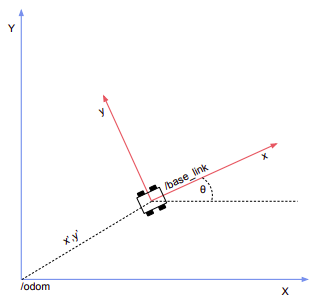
\includegraphics[width=0.75\textwidth]{Images/2-Background/Frames-2021-04-22 12-03-22.png}
	\end{center}
	\caption{\Gls{ROS} frames architecture}% for information sharing\cite{palsson_investigating_2017}}
	\label{fig:ros-frame}
\end{figure}



\chapter{Repository}
\noindent
Everything that has been developed during this thesis could be found in \url{https://github.com/boffomarco/hrp}

The following files are the main contributions provided in this thesis.

\section{System Configuration}
\noindent


.bashrc

network\_file \todo{Configuration of network settings between RPis and PC using ROS to be added in a file describing the procedure}

\section{Localisation Configuration}
\noindent The improved localisation performance are provided using a personalised configuration of the sensors and the related sensor fusion of their measures.

sensors.launch

automower\_safe.launch

imus\_basic.launch

gps.launch

gps.cpp

rs\_camera.launch

rtabmap.launch

BatchEKF.launch

BatchEKF\_last.py

BatchEKF\_lastRPi.py

BatchEKF\_lastSimulated.py

GroundTruthSimulated.py

\section{Mapping Configuration}
\noindent

OccupancyGrid.py

\section{Results Configuration}
\noindent

plot\_histogram.py

gps\_plot.py


\section{Software Configuration}
\noindent
C++ and Python development to work with the ROS framework, explained in details in Appendix \ref{ch:ros}.

Network establishment to communicate wirelessly between Raspberry Pi and computer.

Communication through hotspot



\subsection{Controller}
\label{sec:driver_safe}
\noindent The \gls{ALM} behaviour is defined by the launching file \texttt{automower\_hrp.launch}.
It defines and launch the controller of the \gls{HRP}.



\subsection{Velocity Control}
\label{sec:control}
\noindent
The script \texttt{hrp\_teleop.lauch} as provided by the \gls{HRP} platform is used to drive the \gls{ALM} during the experiments.
It controls the vehicle by setting its desired velocities: $\mathbf{v}v$ and $\boldsymbol \omega$.
In this way it is possible to command the \gls{ALM} to follow a trajectory.


\subsection{Launching the sensors}
\noindent The measurements are obtained from the heterogeneous sensors using the following methods.


The \glspl{IMU} sensors are started using the file \texttt{imus\_basic.launch}.
In this file, the node defined by the \texttt{phidget\_spatial} drivers is used, each sensor will belong to its group, and its coordiante frame is defined by the installation coordinates.

The additional Phidget \gls{GPS} sensors are launched by the file \texttt{imus\_basic.launch}.
In the file, the node calls for a personalised driver that has been implemented to gather the \gls{NMEA} data directly provided by the Phidgets \gls{API}.
The information provided by this \gls{NMEA} data structure

The additional Phidget \gls{GPS} sensors are launched by the file \texttt{imus\_basic.launch}.
In the file, the node calls for a personalised driver that has been implemented to gather the \gls{NMEA} data directly through the Phidgets \gls{API}.
The information provided by this \gls{NMEA} data structure covers both the localisation estimate and its related accuracy, in form of \gls{HDOP}.

The camera added is exploited running the file \texttt{rs\_camera.launch}.
It is a customised launch file that has been improved starting from the camera own driver.
As it does not provide the measurements directly, the \gls{VO} package \gls{RTABMAP} is run via a customised \texttt{rtabmap.launch} file, obtained initially from the \gls{RTABMAP} package and then tuned for the scope of this thesis.



\subsection{Launching the localisation feature}
\noindent The localisation improvements are performed by the script in \texttt{AEKF.py}.
It performs the \gls{AEKF} elaborated in \ref{sec:locConf}.

To perform in an asynchronous way, a binary lock is adopted to account when a measurement update is performed at the same time of a measurement receive.


\subsection{Launching the mapping update}
\noindent The mapping feature is provided by the implementation available in \texttt{Mapping.py}.

The initial phase is of setting the boundaries.

Then a specific message changes the

The collision events are then exploited to update the knowledge of the surroundings.




%\chapter{Something Extra}


\end{sloppypar}

\label{pg:lastPageofMainmatter}

\clearpage
\section*{For DIVA}
\divainfo{pg:lastPageofPreface}{pg:lastPageofMainmatter}



\includepdf[pages=2]{Input/kth-cover.pdf}
\end{document}
